\documentclass[11pt]{article}
\usepackage[utf8]{inputenc}
\usepackage{amsmath}
\usepackage{natbib}
\usepackage{graphicx}
%\usepackage[spanish, es-minimal]{babel}
\usepackage[spanish, es-minimal, english]{babel}
%\usepackage[vmargin=0.8in, hmargin=1.00in]{geometry}
\usepackage[vmargin=0.7in, hmargin=1.0in]{geometry}
\usepackage{lipsum}
\usepackage{longtable}
\usepackage{pdfpages}
\usepackage{listings}
\usepackage{hyperref}
\usepackage{url}

\newcommand\U[1]{\ensuremath{\mathrm{#1}}}
\newcommand\K{\U{K}}
\newcommand\cm{\U{cm}}
\newcommand\AU{\U{AU}}
\newcommand\g{\U{g}}
\newcommand\msolagno{M_\odot\,\U{yr^{-1}}}

\newcommand\acre{\ensuremath{_{\mathrm{acre}}}}
\newcommand\eff{\ensuremath{_{\mathrm{eff}}}}
\newcommand\Int{\ensuremath{_{\mathrm{Int}}}}
\newcommand\Ext{\ensuremath{_{\mathrm{Ext}}}}

\newcommand\BowshockFig[1]{
  \includegraphics[width=\figwidth, clip, trim=10 10 10 10]
  {#1}
}
\newcommand\raiselabel[1]{\raisebox{0.9\figwidth}[-0.5\figwidth]{#1}}
\newcommand\raiselabelPho[1]{\raisebox{0.62\figwidth}[-0.5\figwidth]{#1}}



\title{Planetary nebulae in DR2 J-PLUS }

%\author{
   %Bolsista: Luis Angel Gutiérrez Soto\\
   %Coordenadora: Claudia Lucia Mendes de Oliveira 
%}
\date{}

\begin{document}
\maketitle

\begin{figure}
\centering
\begin{tabular}{l l}
  \includegraphics[width=0.5\linewidth, trim=10 15 5 8, clip]{../../../Dropbox/JPAS/Tesis/Fig/DdDm-1-HPNe-SPLUS18-magnitude-paper.pdf}
   \includegraphics[width=0.52\linewidth, trim=5 15 5 8, clip]{../../../Dropbox/JPAS/Tesis/Fig/DdDm1_L4_T200_output_SED-tere_E02_600-JPLUS17-magnitude-paper.pdf}
  \end{tabular}  
\end{figure}

\begin{figure*}
%\setlength\tabcolsep{\figstampcolsep}
\centering
\begin{tabular}{l l}
 \includegraphics[width=0.5\linewidth, trim=10 10 10 10, clip]{../../../Dropbox/JPAS/Tesis/Fig/Fig1-JPLUS17-Viironen.pdf} & \\
 \includegraphics[width=0.5\linewidth, trim=10 10 10 10, clip]{../../../Dropbox/JPAS/Tesis/Fig/Fig2-JPLUS17-J0515-J0660.pdf} & \includegraphics[width=0.5\linewidth, trim=10 10 10 10, clip]{../../../Dropbox/JPAS/Tesis/Fig/Fig5-JPLUS17-J0660-r.pdf} \\
%\raiselabel{(\textit{a})} & \raiselabel{(\textit{b})}\\
\includegraphics[width=0.5\linewidth, trim=10 10 10 10, clip]{../../../Dropbox/JPAS/Tesis/Fig/Fig3-JPLUS17-z-g.pdf} & \includegraphics[width=0.5\linewidth, trim=10 10 10 10, clip]{../../../Dropbox/JPAS/Tesis/Fig/Fig6-JPLUS17-g-i.pdf} \\
%\raiselabel{(\textit{c})} & \raiselabel{(\textit{d})}
  
  \end{tabular}
\end{figure*}

\begin{figure*}
%\setlength\tabcolsep{\figstampcolsep}
\centering
\begin{tabular}{l l}
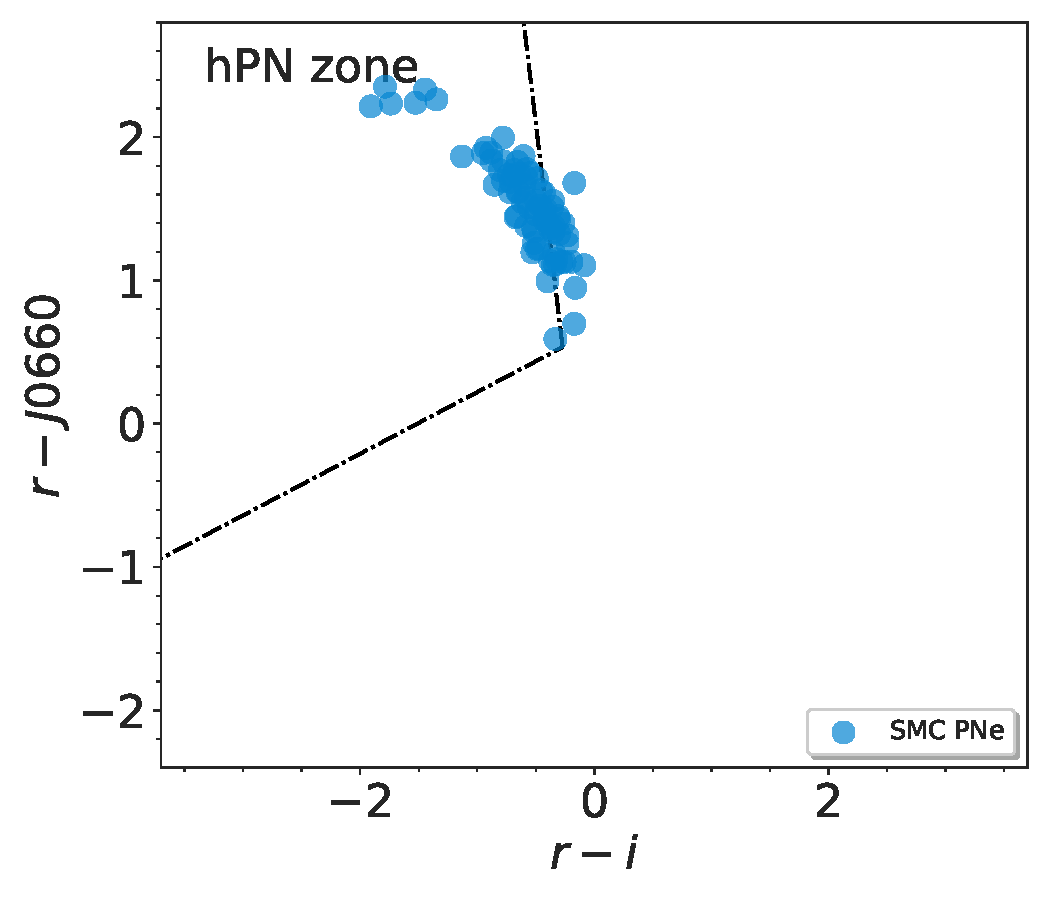
\includegraphics[width=0.5\linewidth, trim=10 10 10 10, clip]{figs-pca/Fig1-PN-pc-Halpha_emitters_threeerror-cleaning-limfilter-limcolor-flags-mask-broad-vironen.pdf} & \\
 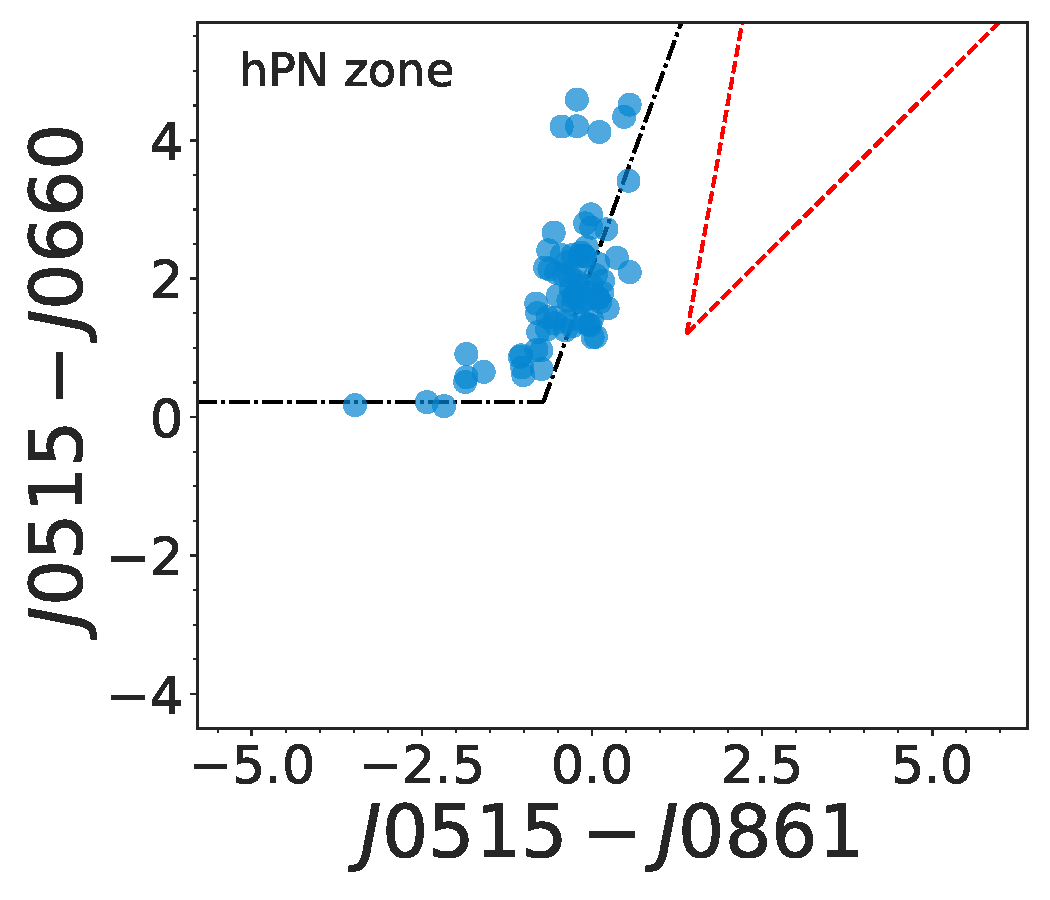
\includegraphics[width=0.5\linewidth, trim=10 10 10 10, clip]{figs-pca/Fig2-PN-pc-Halpha_emitters_threeerror-cleaning-limfilter-limcolor-flags-mask-broad-J0515_J0660.pdf} & 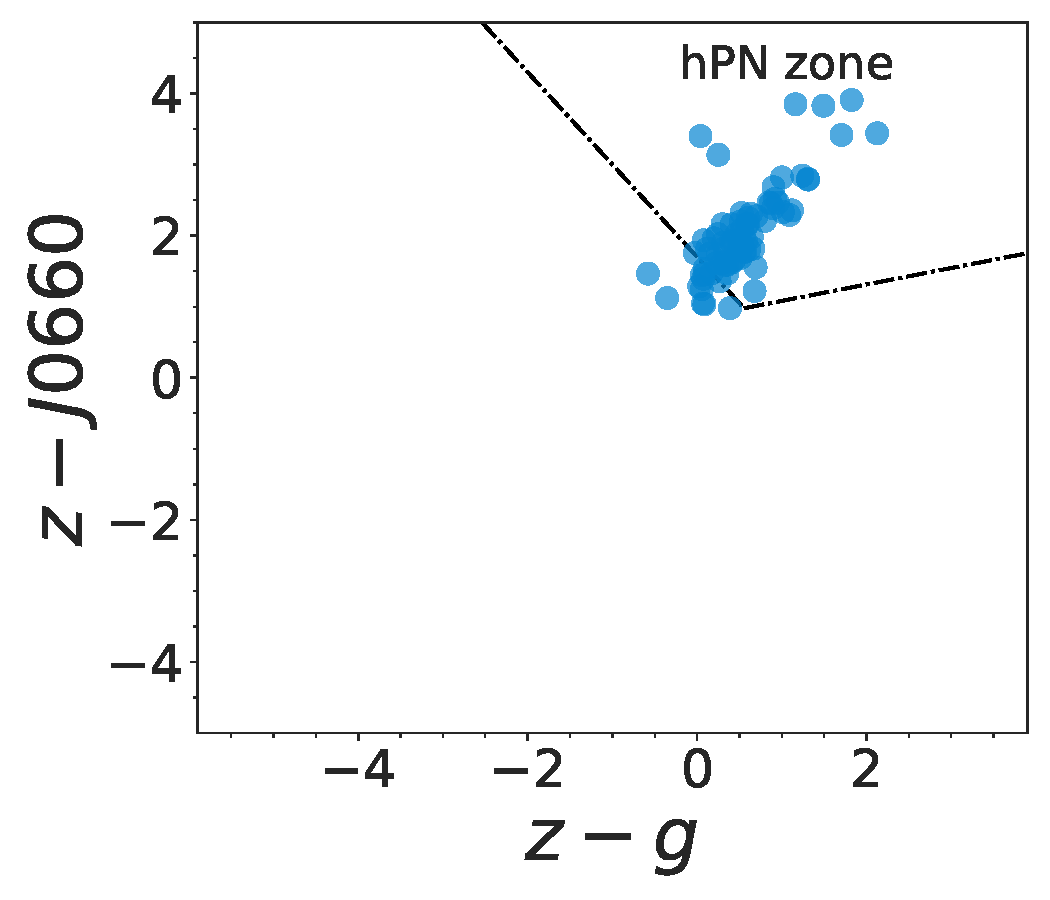
\includegraphics[width=0.5\linewidth, trim=10 10 10 10, clip]{figs-pca/Fig3-PN-pc-Halpha_emitters_threeerror-cleaning-limfilter-limcolor-flags-mask-broad-z.pdf} \\
%\raiselabel{(\textit{a})} & \raiselabel{(\textit{b})}\\
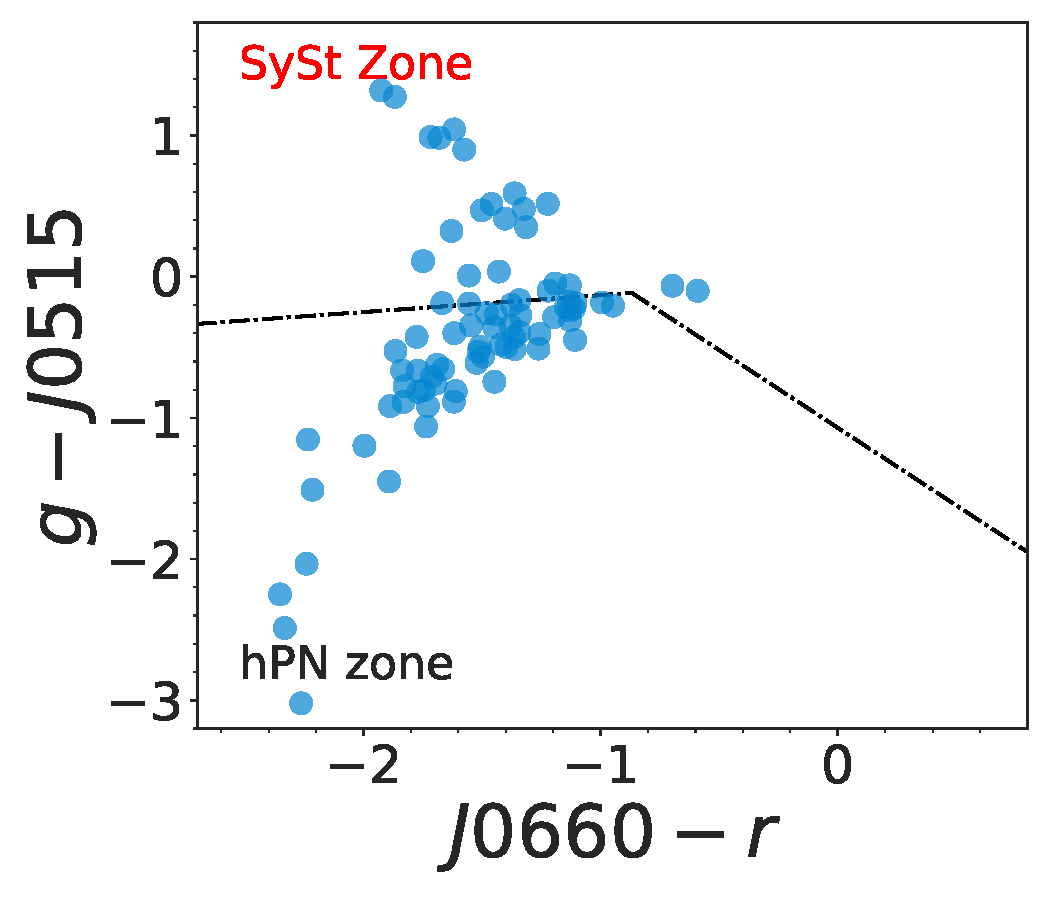
\includegraphics[width=0.5\linewidth, trim=10 10 10 10, clip]{figs-pca/Fig4-PN-pc-Halpha_emitters_threeerror-cleaning-limfilter-limcolor-flags-mask-broad-g.pdf} & 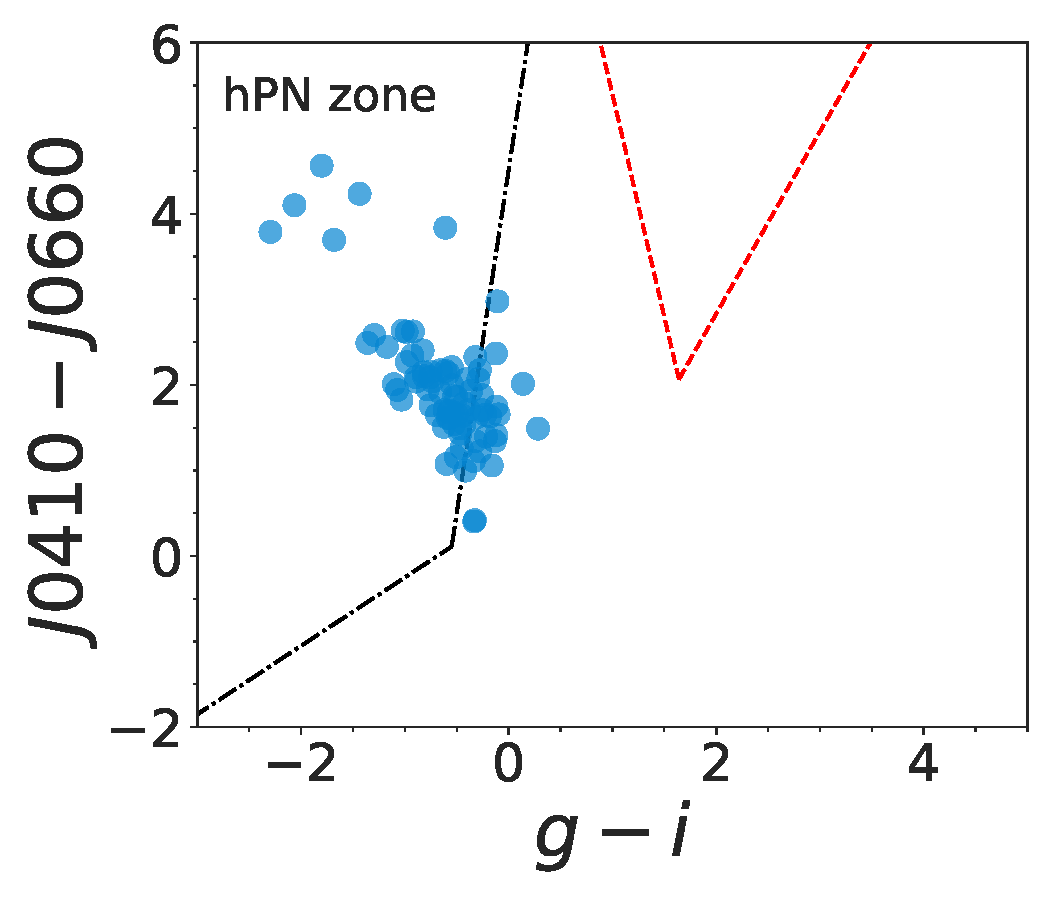
\includegraphics[width=0.5\linewidth, trim=10 10 10 10, clip]{figs-pca/Fig5-PN-pc-Halpha_emitters_threeerror-cleaning-limfilter-limcolor-flags-mask-broad-gi.pdf} \\
%\raiselabel{(\textit{c})} & \raiselabel{(\textit{d})}
\end{tabular}
\caption{}
\label{fig:smppne}
\end{figure*}

 (see Fig.~\ref{fig:smppne}),

\newpage
\begin{longtable}{ccc}
  % \begin{table}
% \begin{tabular}{ccc}
\textbf{Aper (6 ")} & \textbf{J0515+J0660+J0861} & \textbf{gSDSS+rSDSS+iSDSS} \\
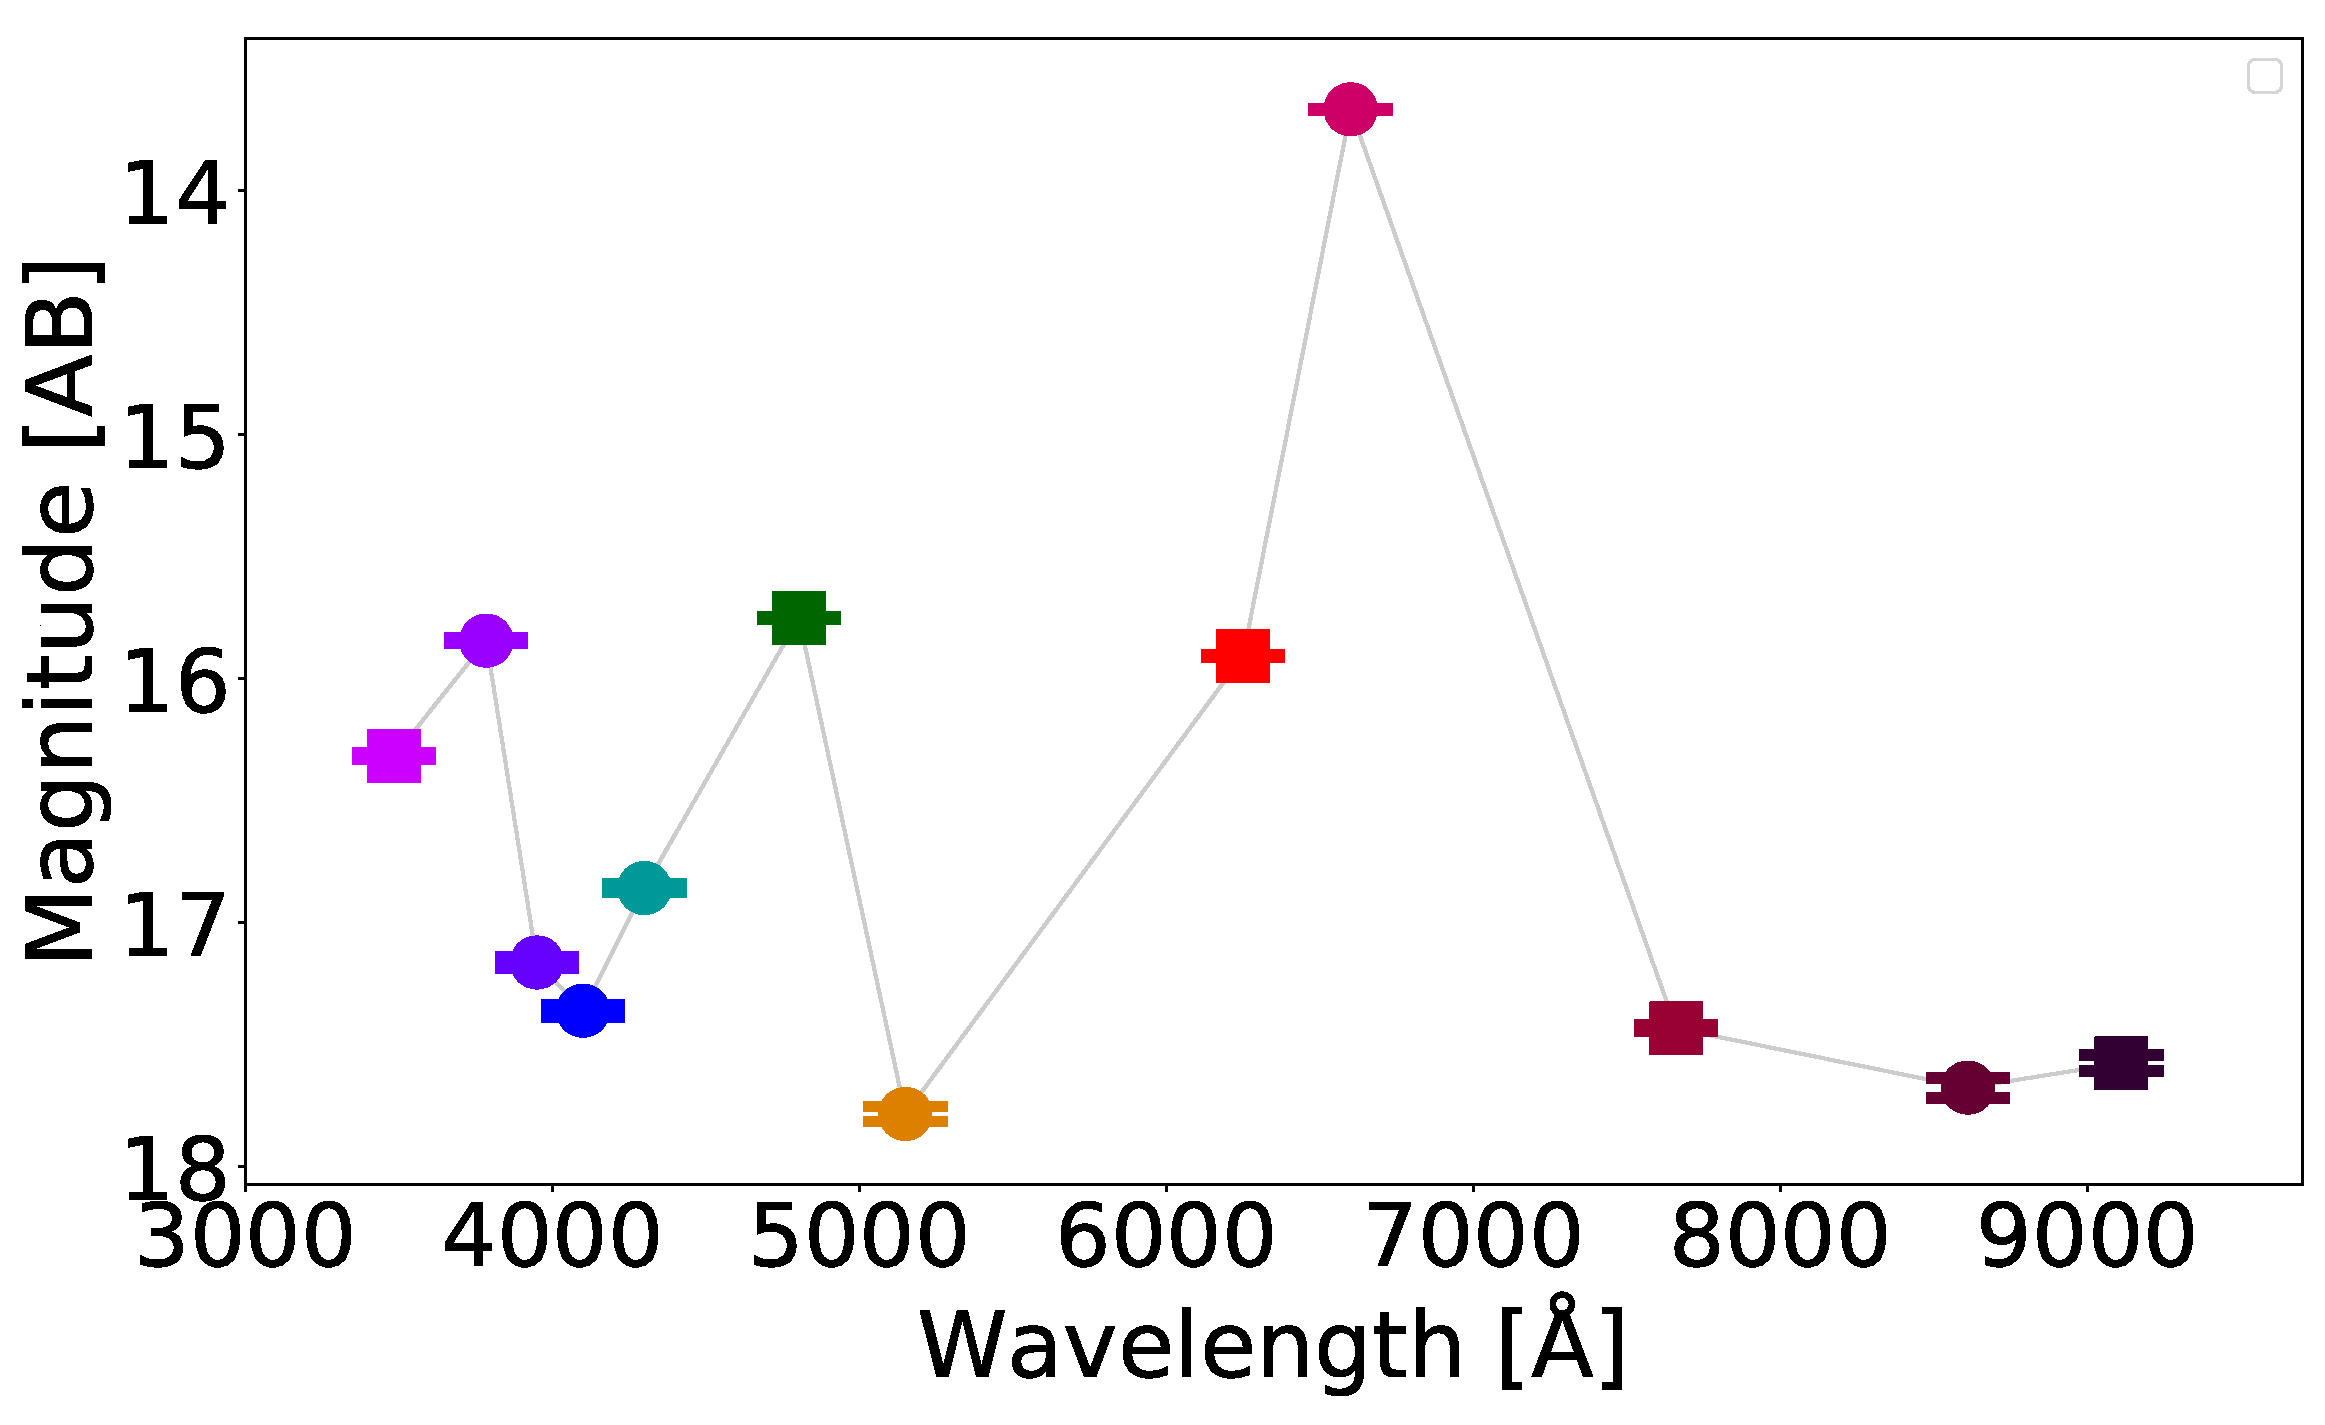
\includegraphics[width=0.3\linewidth, clip]{figs-pca/photospectrum_62617-9746-PN-pc-Halpha_emitters_threeerror-cleaning-limfilter-limcolor-flags-mask-broad_MAG_APER_6_0.pdf} & 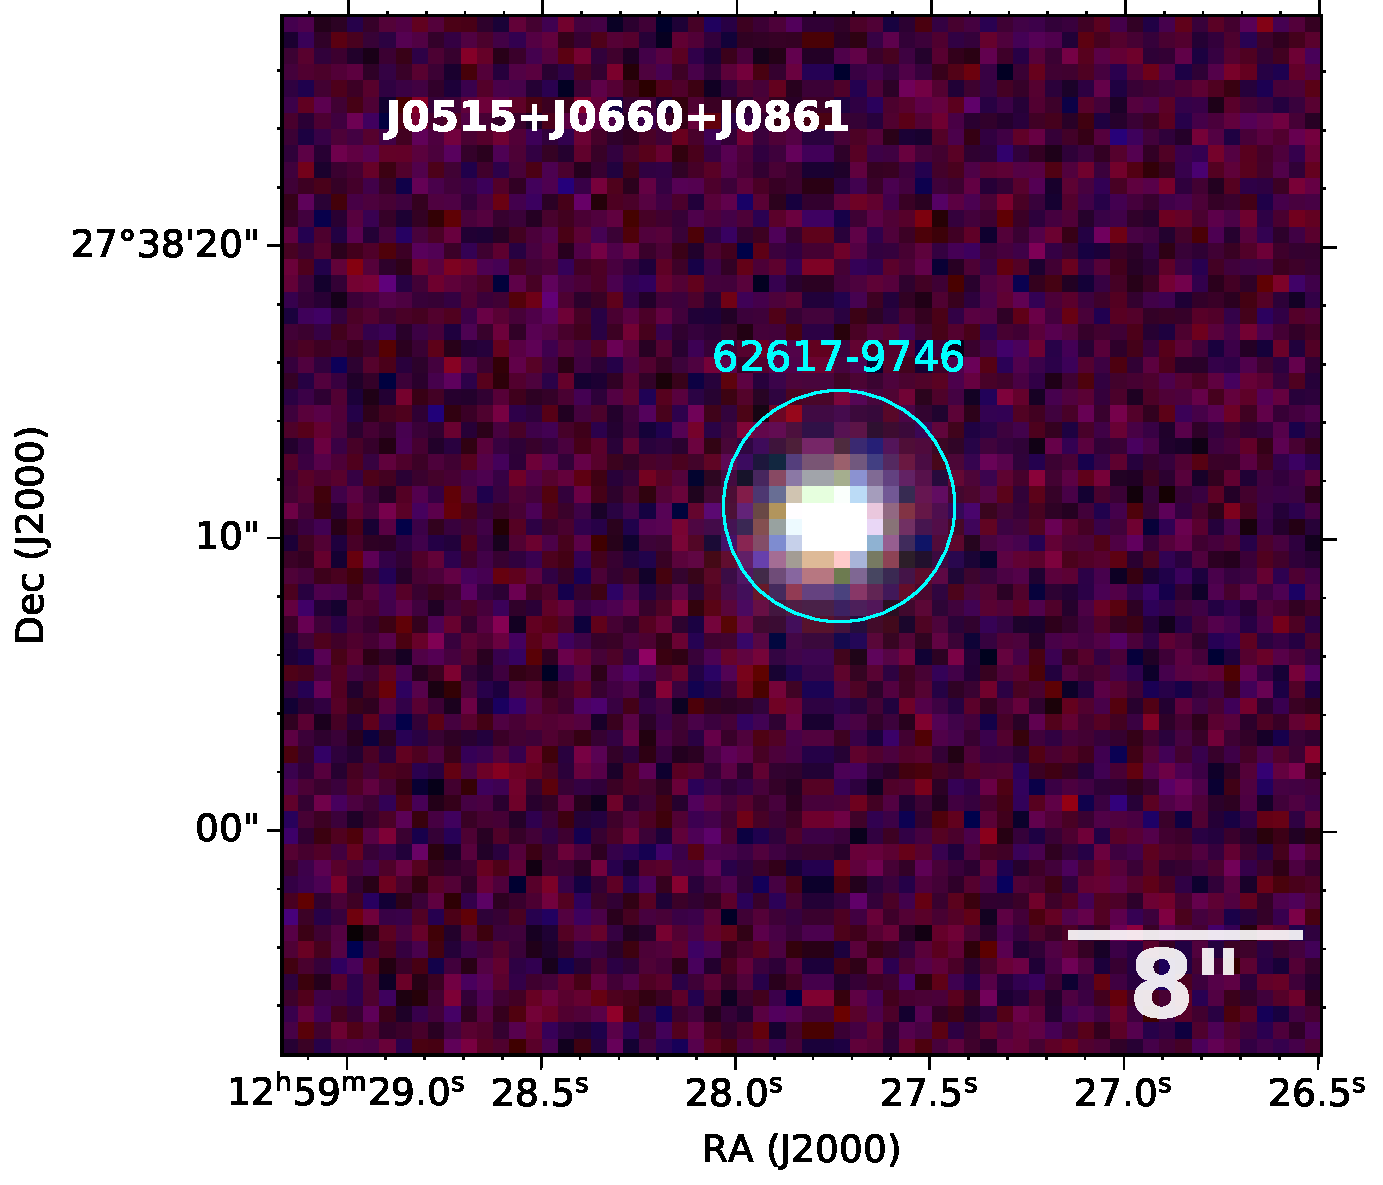
\includegraphics[width=0.3\linewidth, clip]{Field_62617/1000001-JPLUS-00588-v202006_J0861_62617-9746-RGB.pdf} & 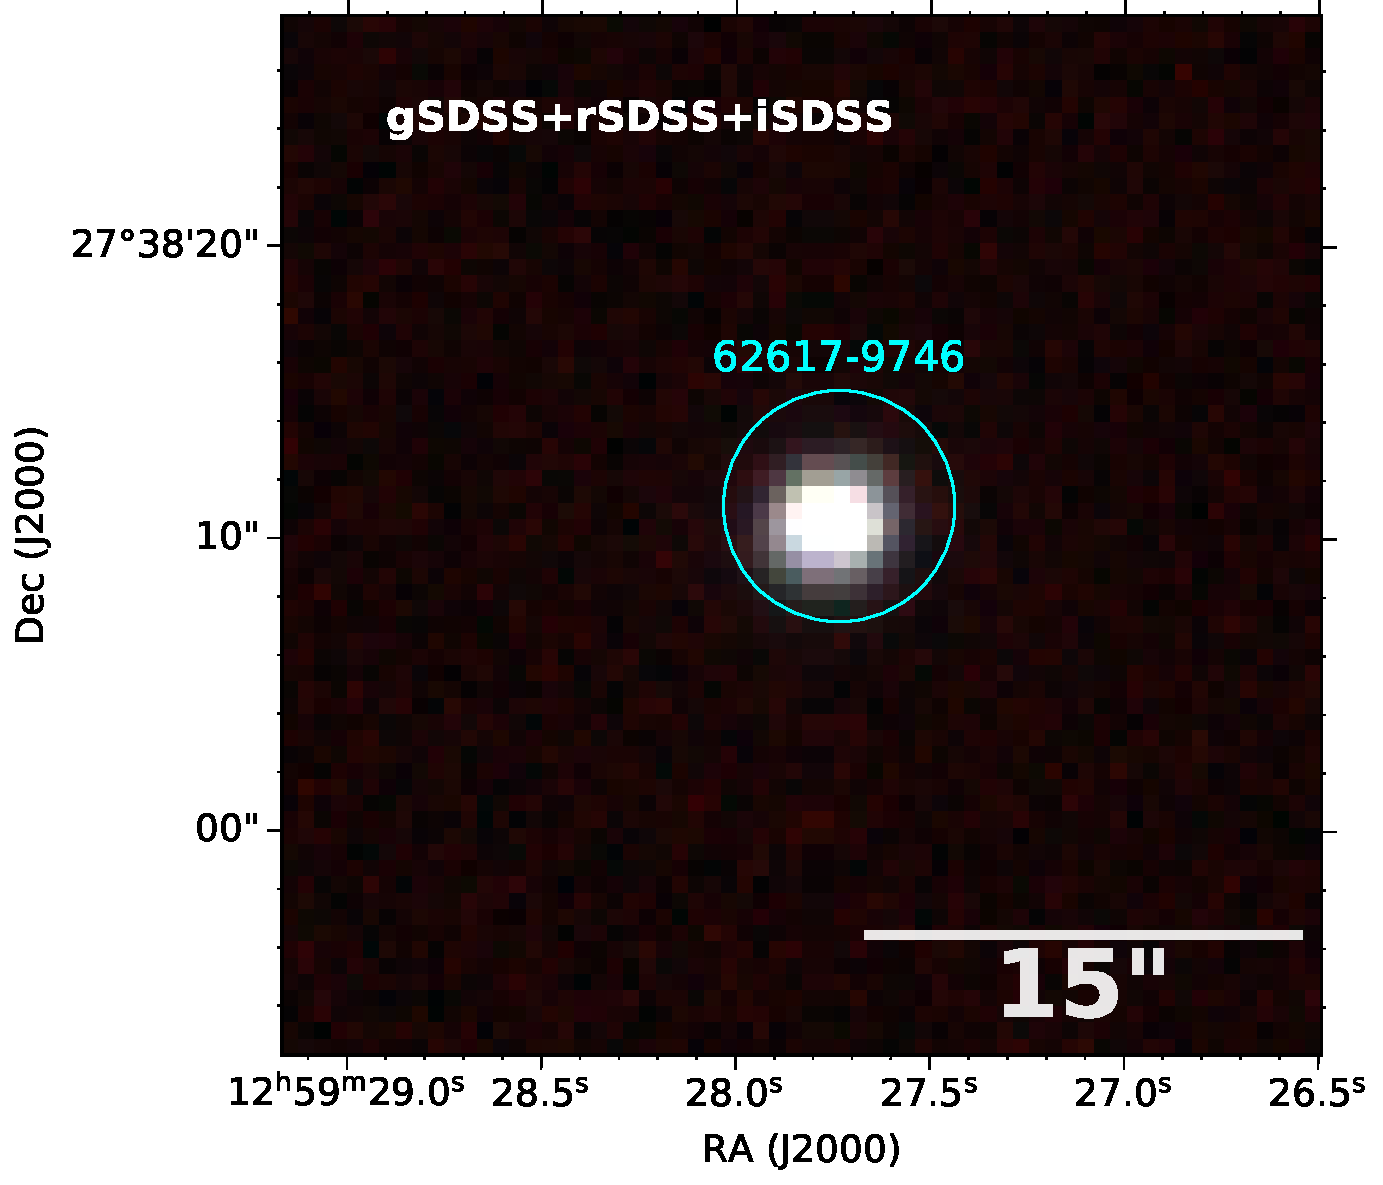
\includegraphics[width=0.3\linewidth, clip]{Field_62617/1000001-JPLUS-00588-v202006_iSDSS_62617-9746-RGB.pdf} \\
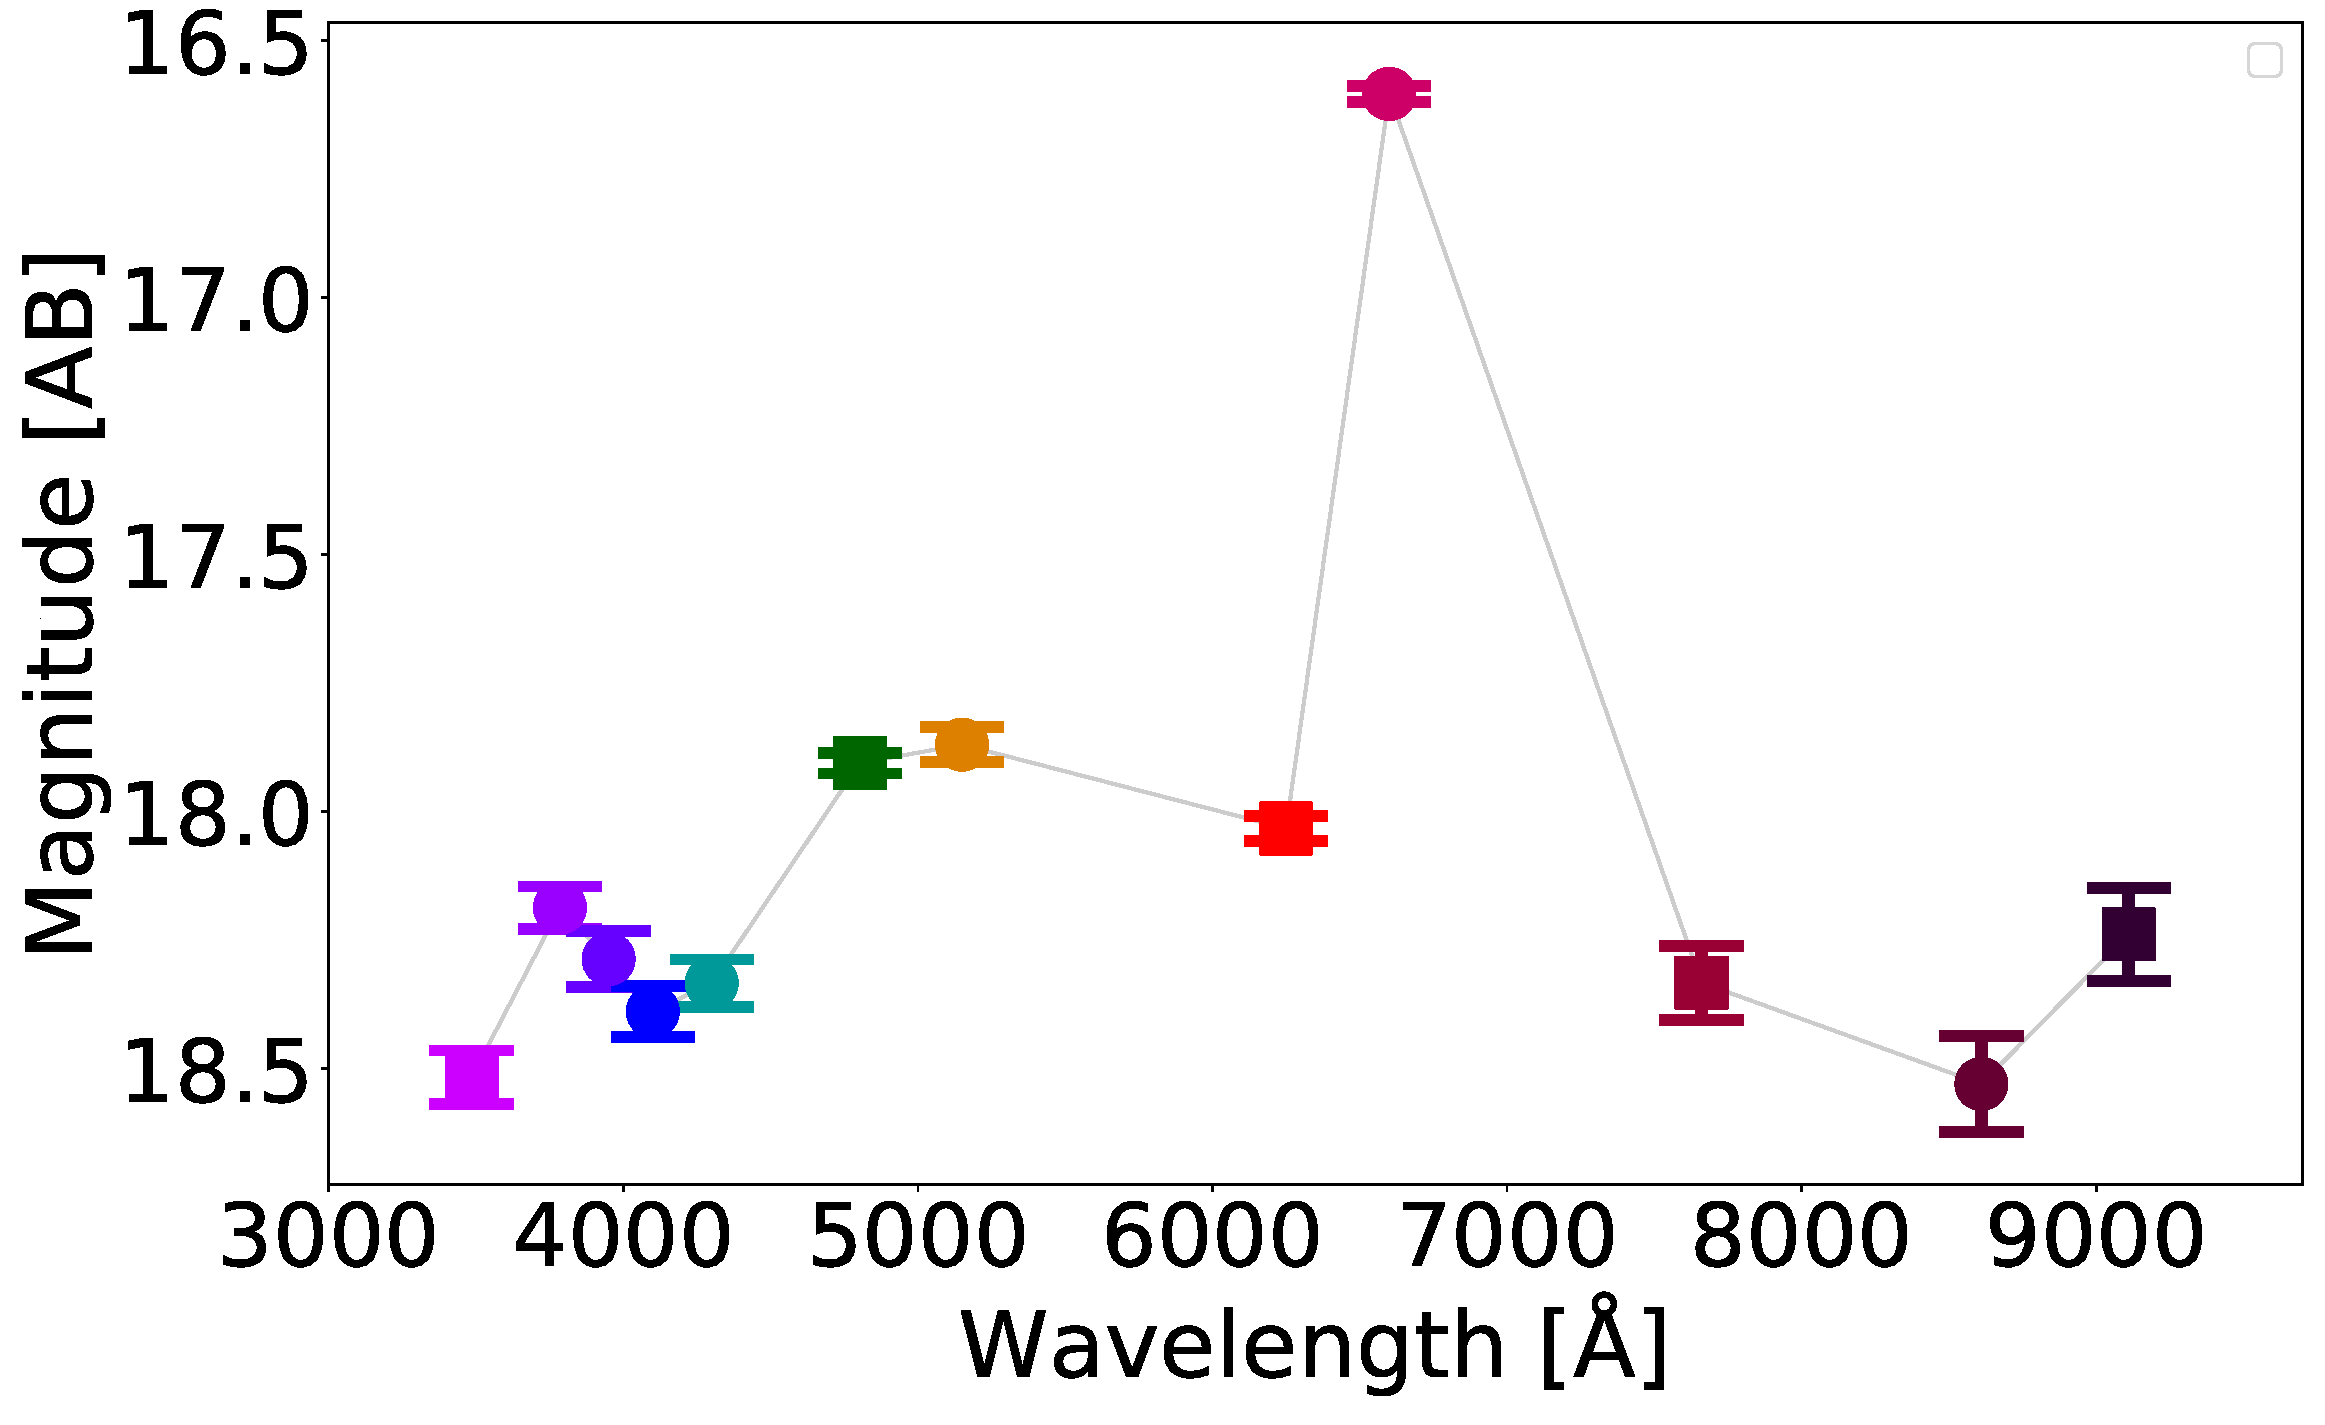
\includegraphics[width=0.3\linewidth, clip]{figs-pca/photospectrum_63236-4396-PN-pc-Halpha_emitters_threeerror-cleaning-limfilter-limcolor-flags-mask-broad_MAG_APER_6_0.pdf} & 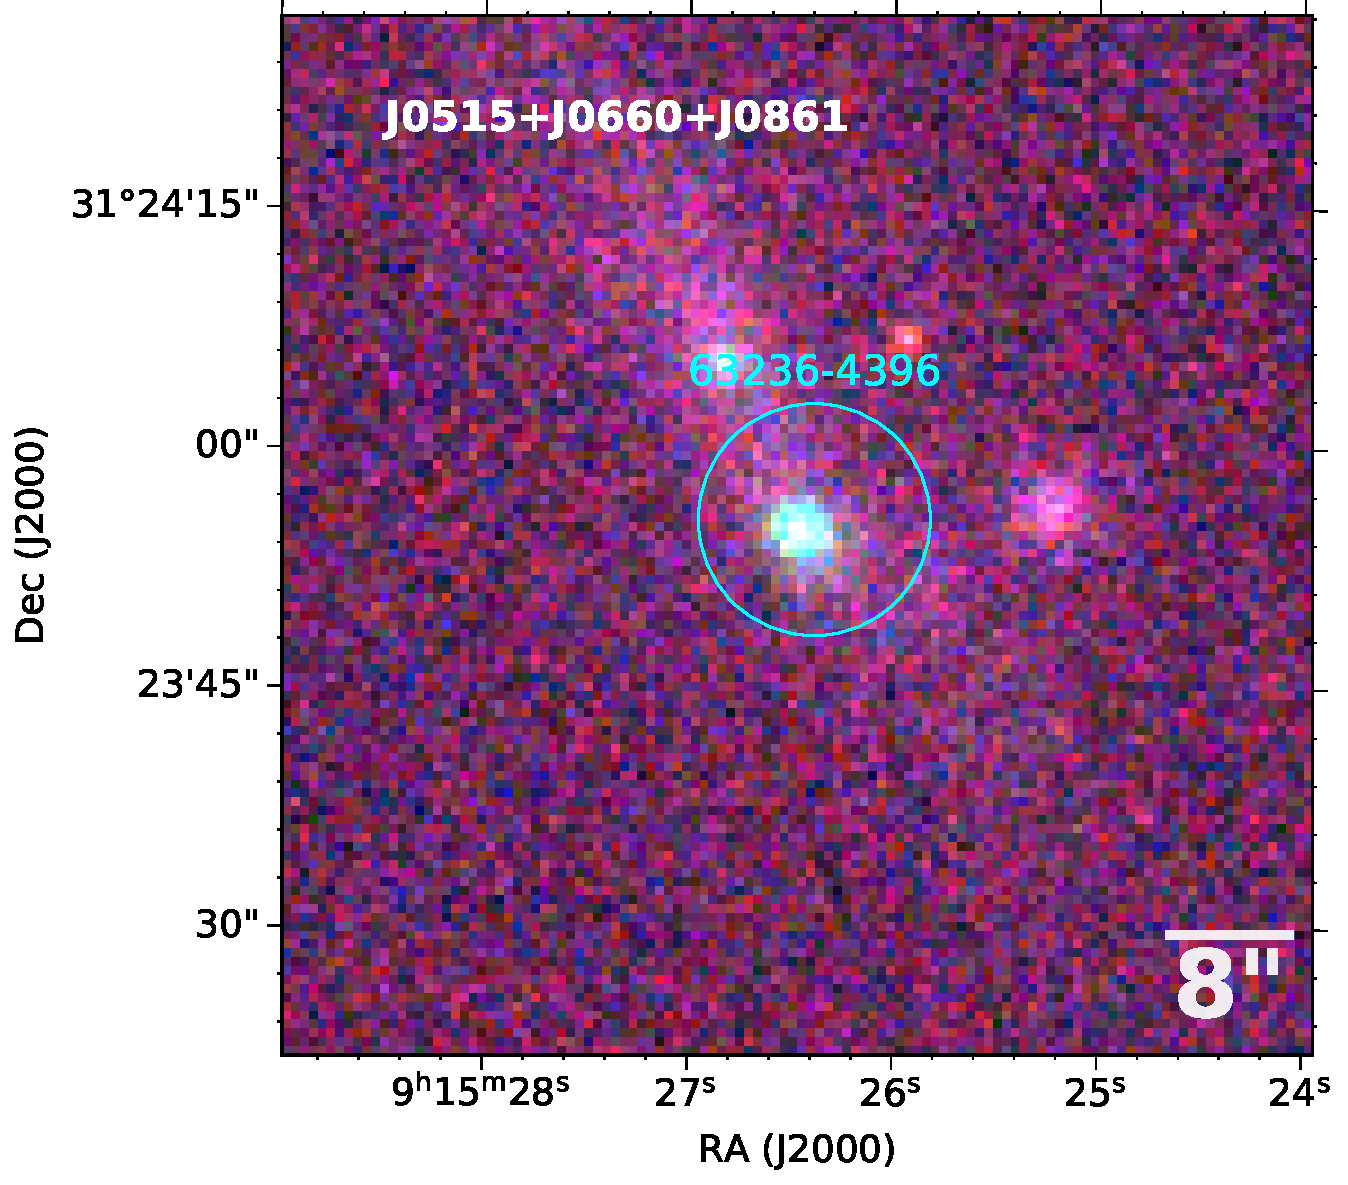
\includegraphics[width=0.3\linewidth, clip]{Field_63236/1000001-JPLUS-00867-v202006_J0861_63236-4396-RGB.pdf} & 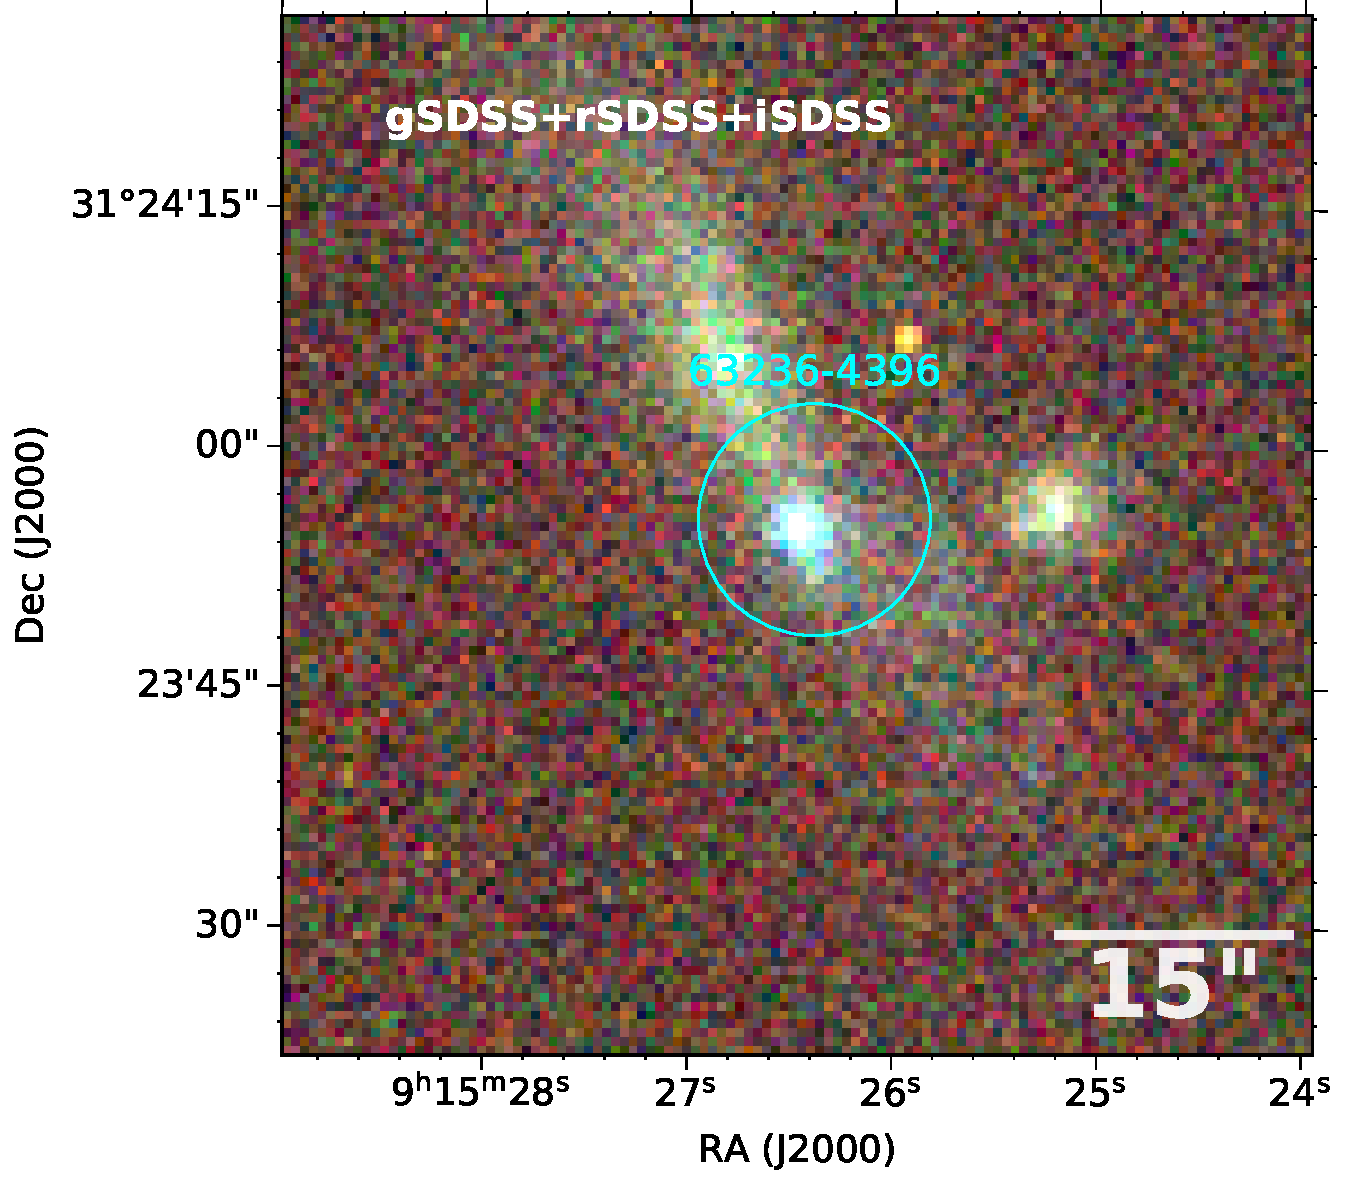
\includegraphics[width=0.3\linewidth, clip]{Field_63236/1000001-JPLUS-00867-v202006_iSDSS_63236-4396-RGB.pdf} \\
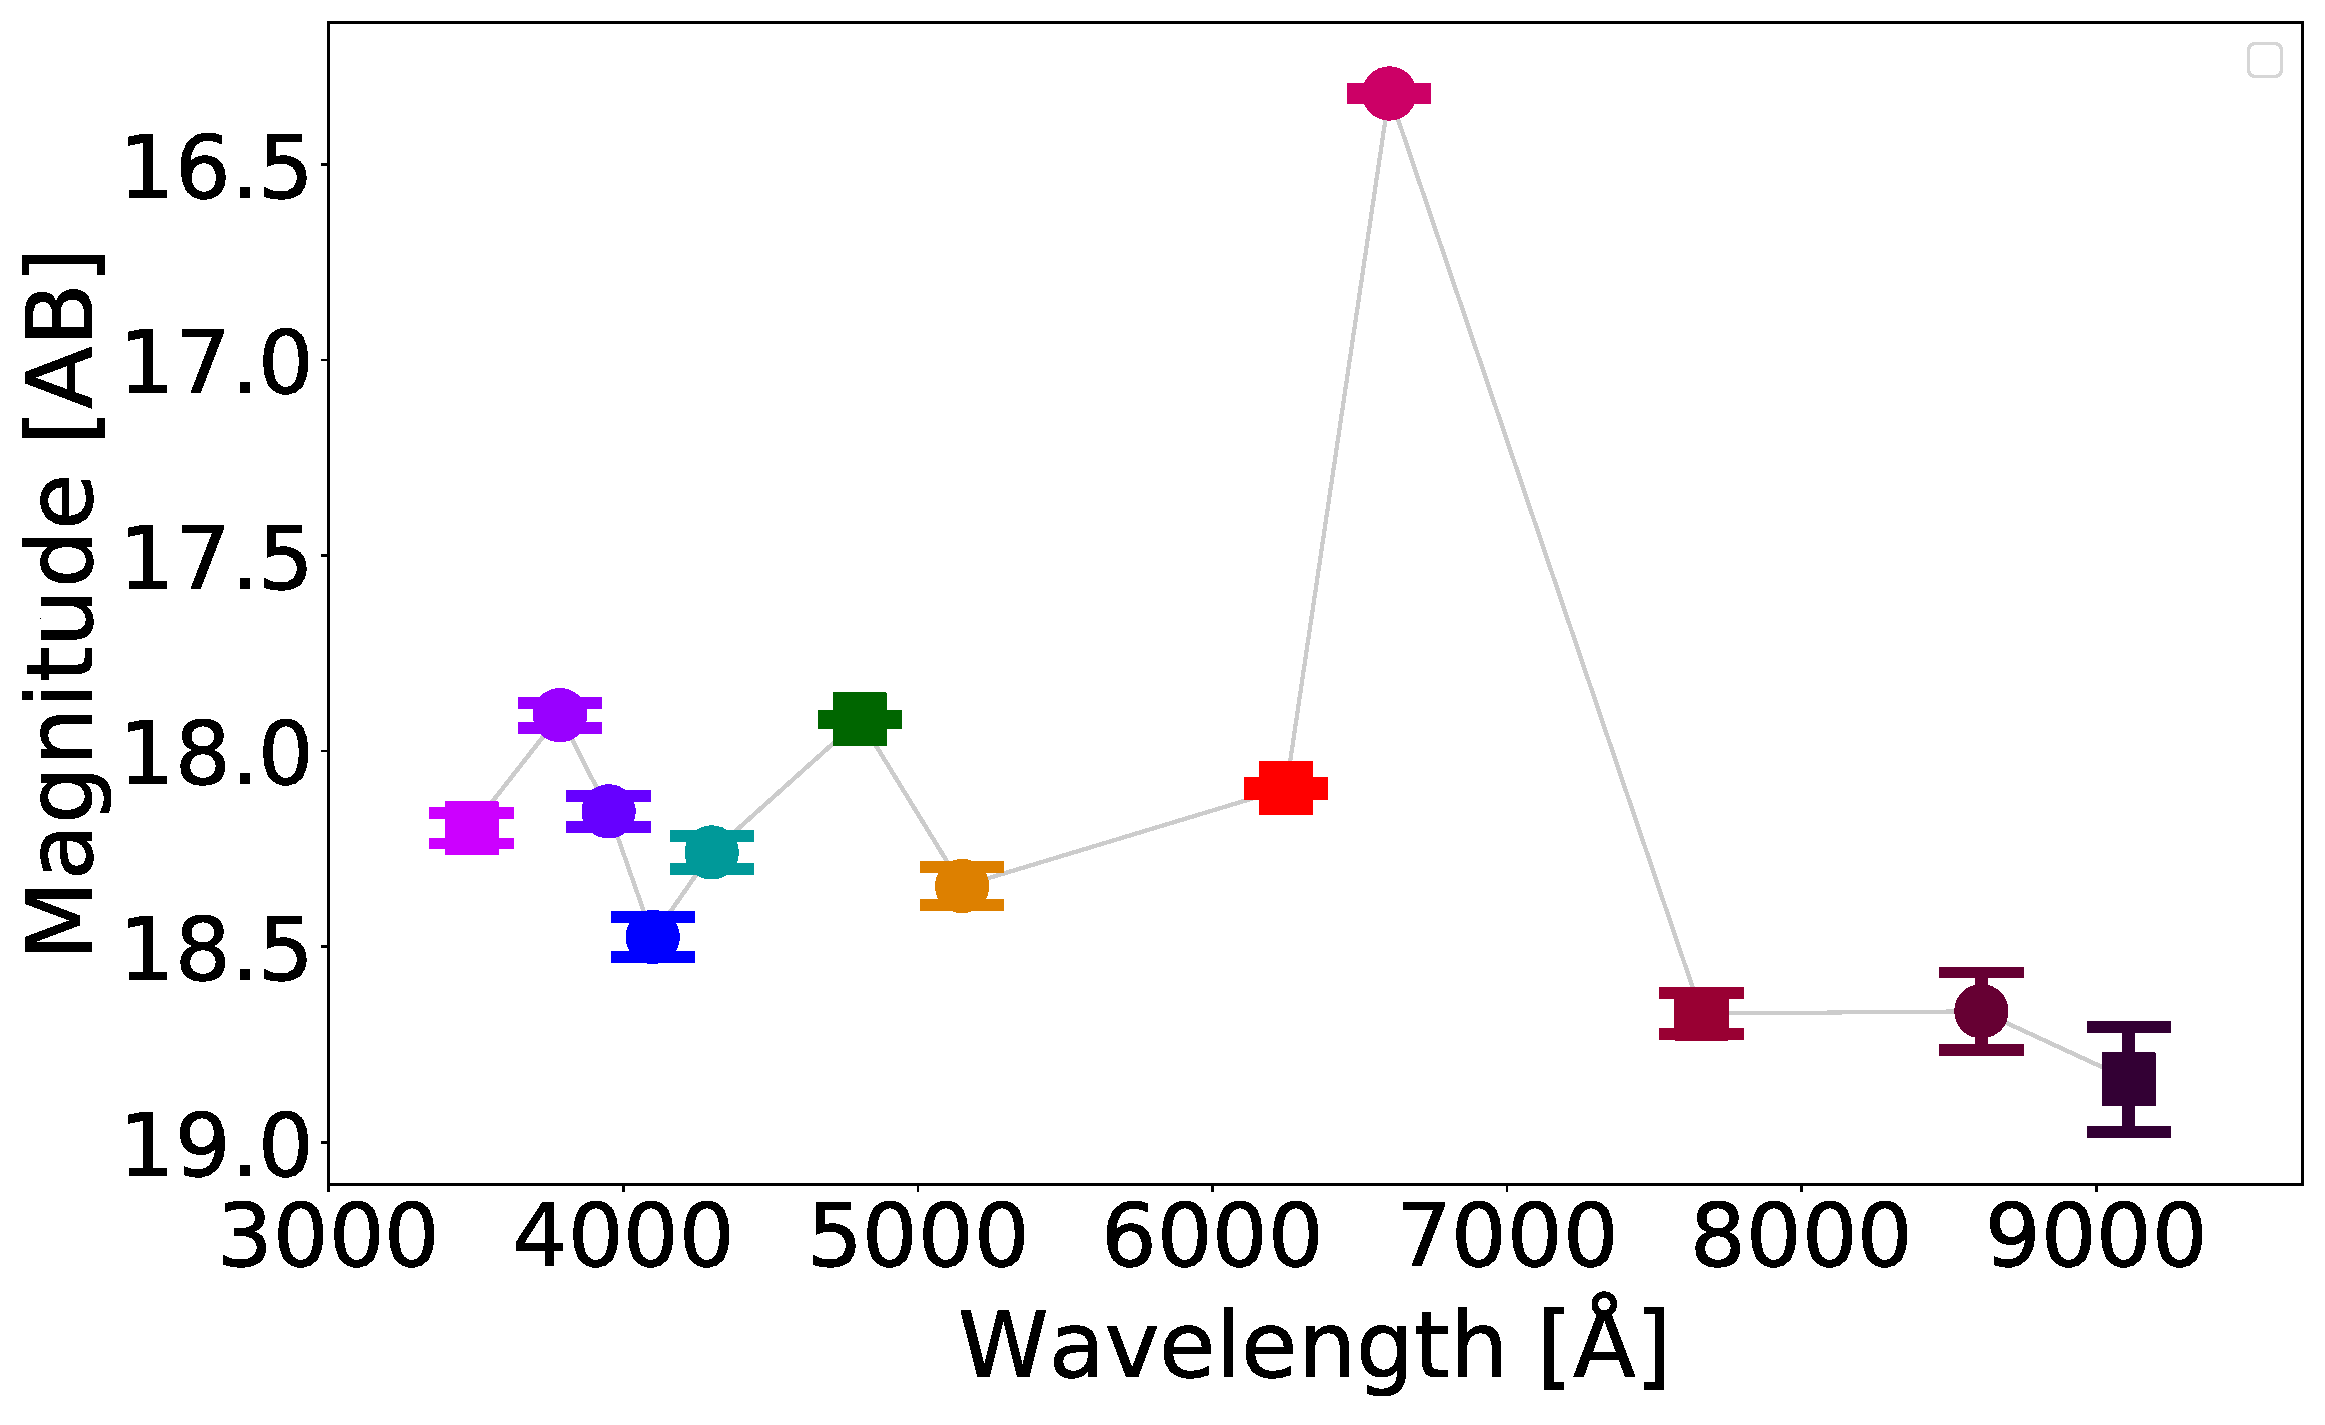
\includegraphics[width=0.3\linewidth, clip]{figs-pca/photospectrum_63308-6151-PN-pc-Halpha_emitters_threeerror-cleaning-limfilter-limcolor-flags-mask-broad_MAG_APER_6_0.pdf} & 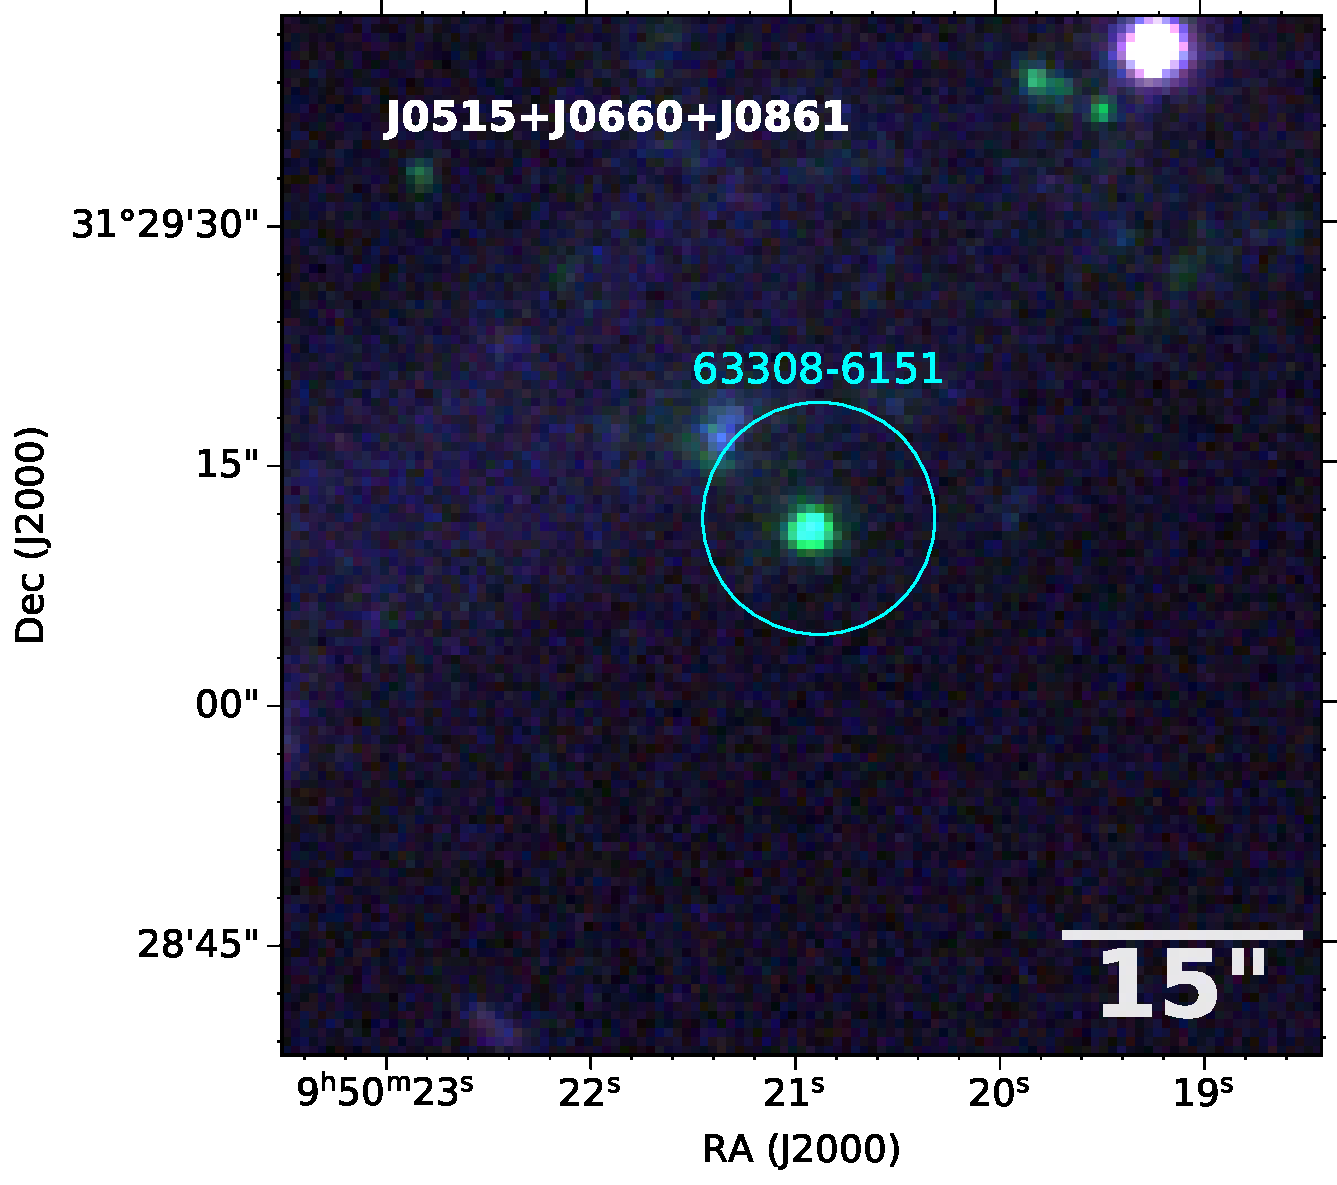
\includegraphics[width=0.3\linewidth, clip]{Field_63308/1000001-JPLUS-00873-v202006_J0861_63308-6151-RGB.pdf} & 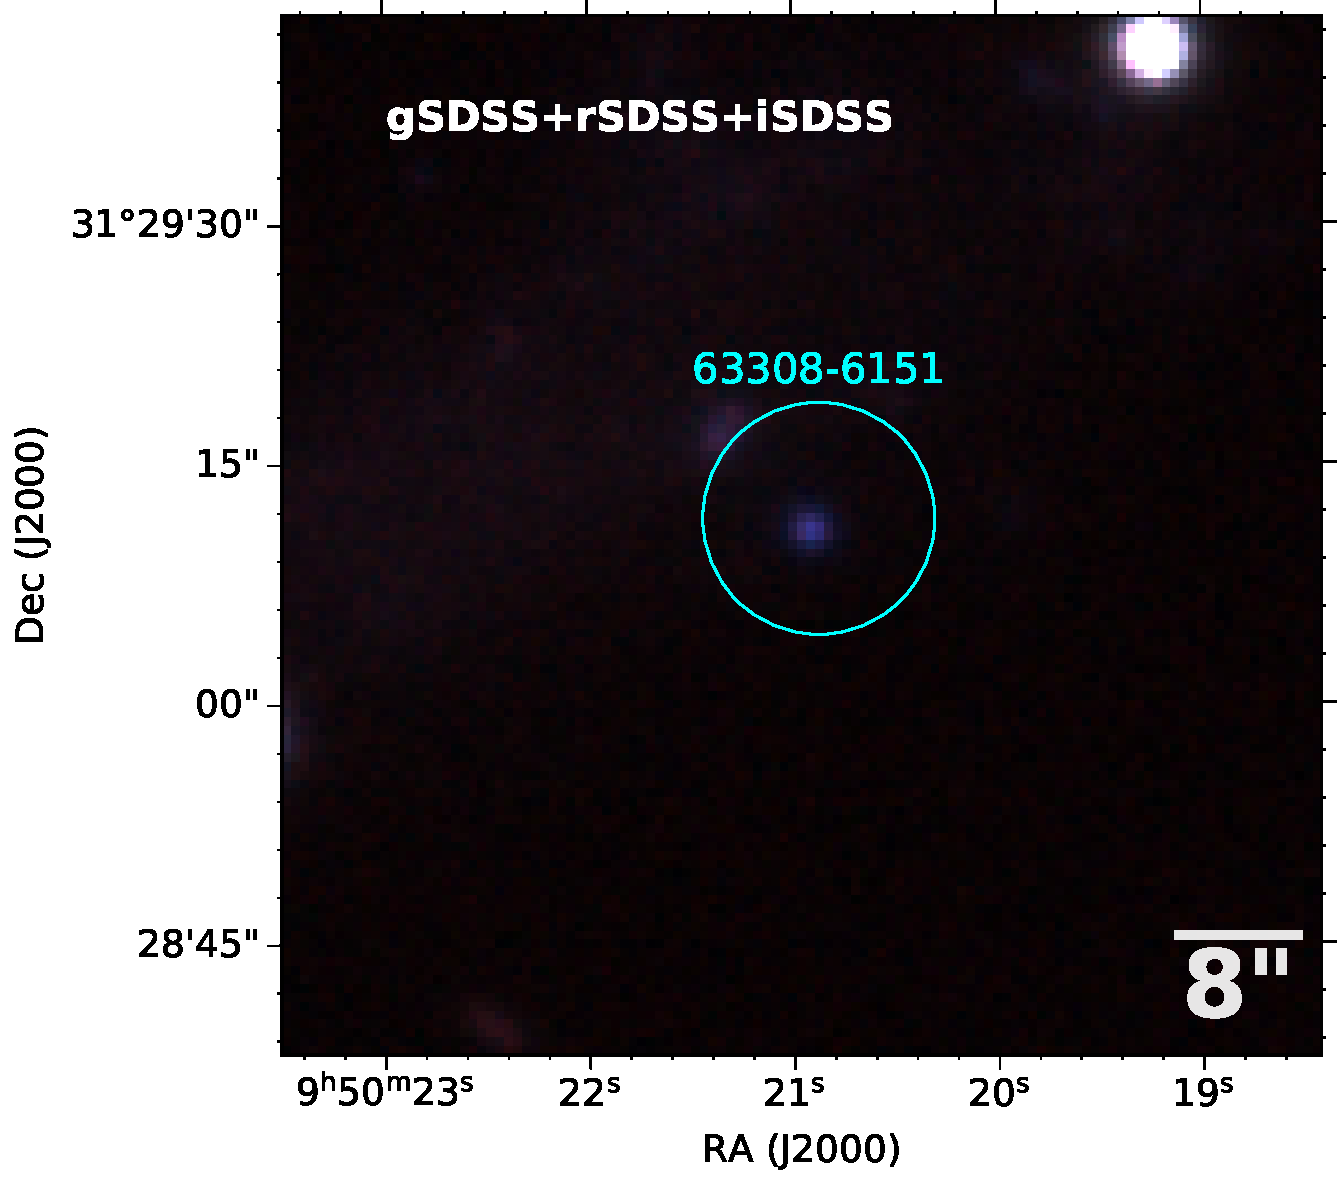
\includegraphics[width=0.3\linewidth, clip]{Field_63308/1000001-JPLUS-00873-v202006_iSDSS_63308-6151-RGB.pdf} \\
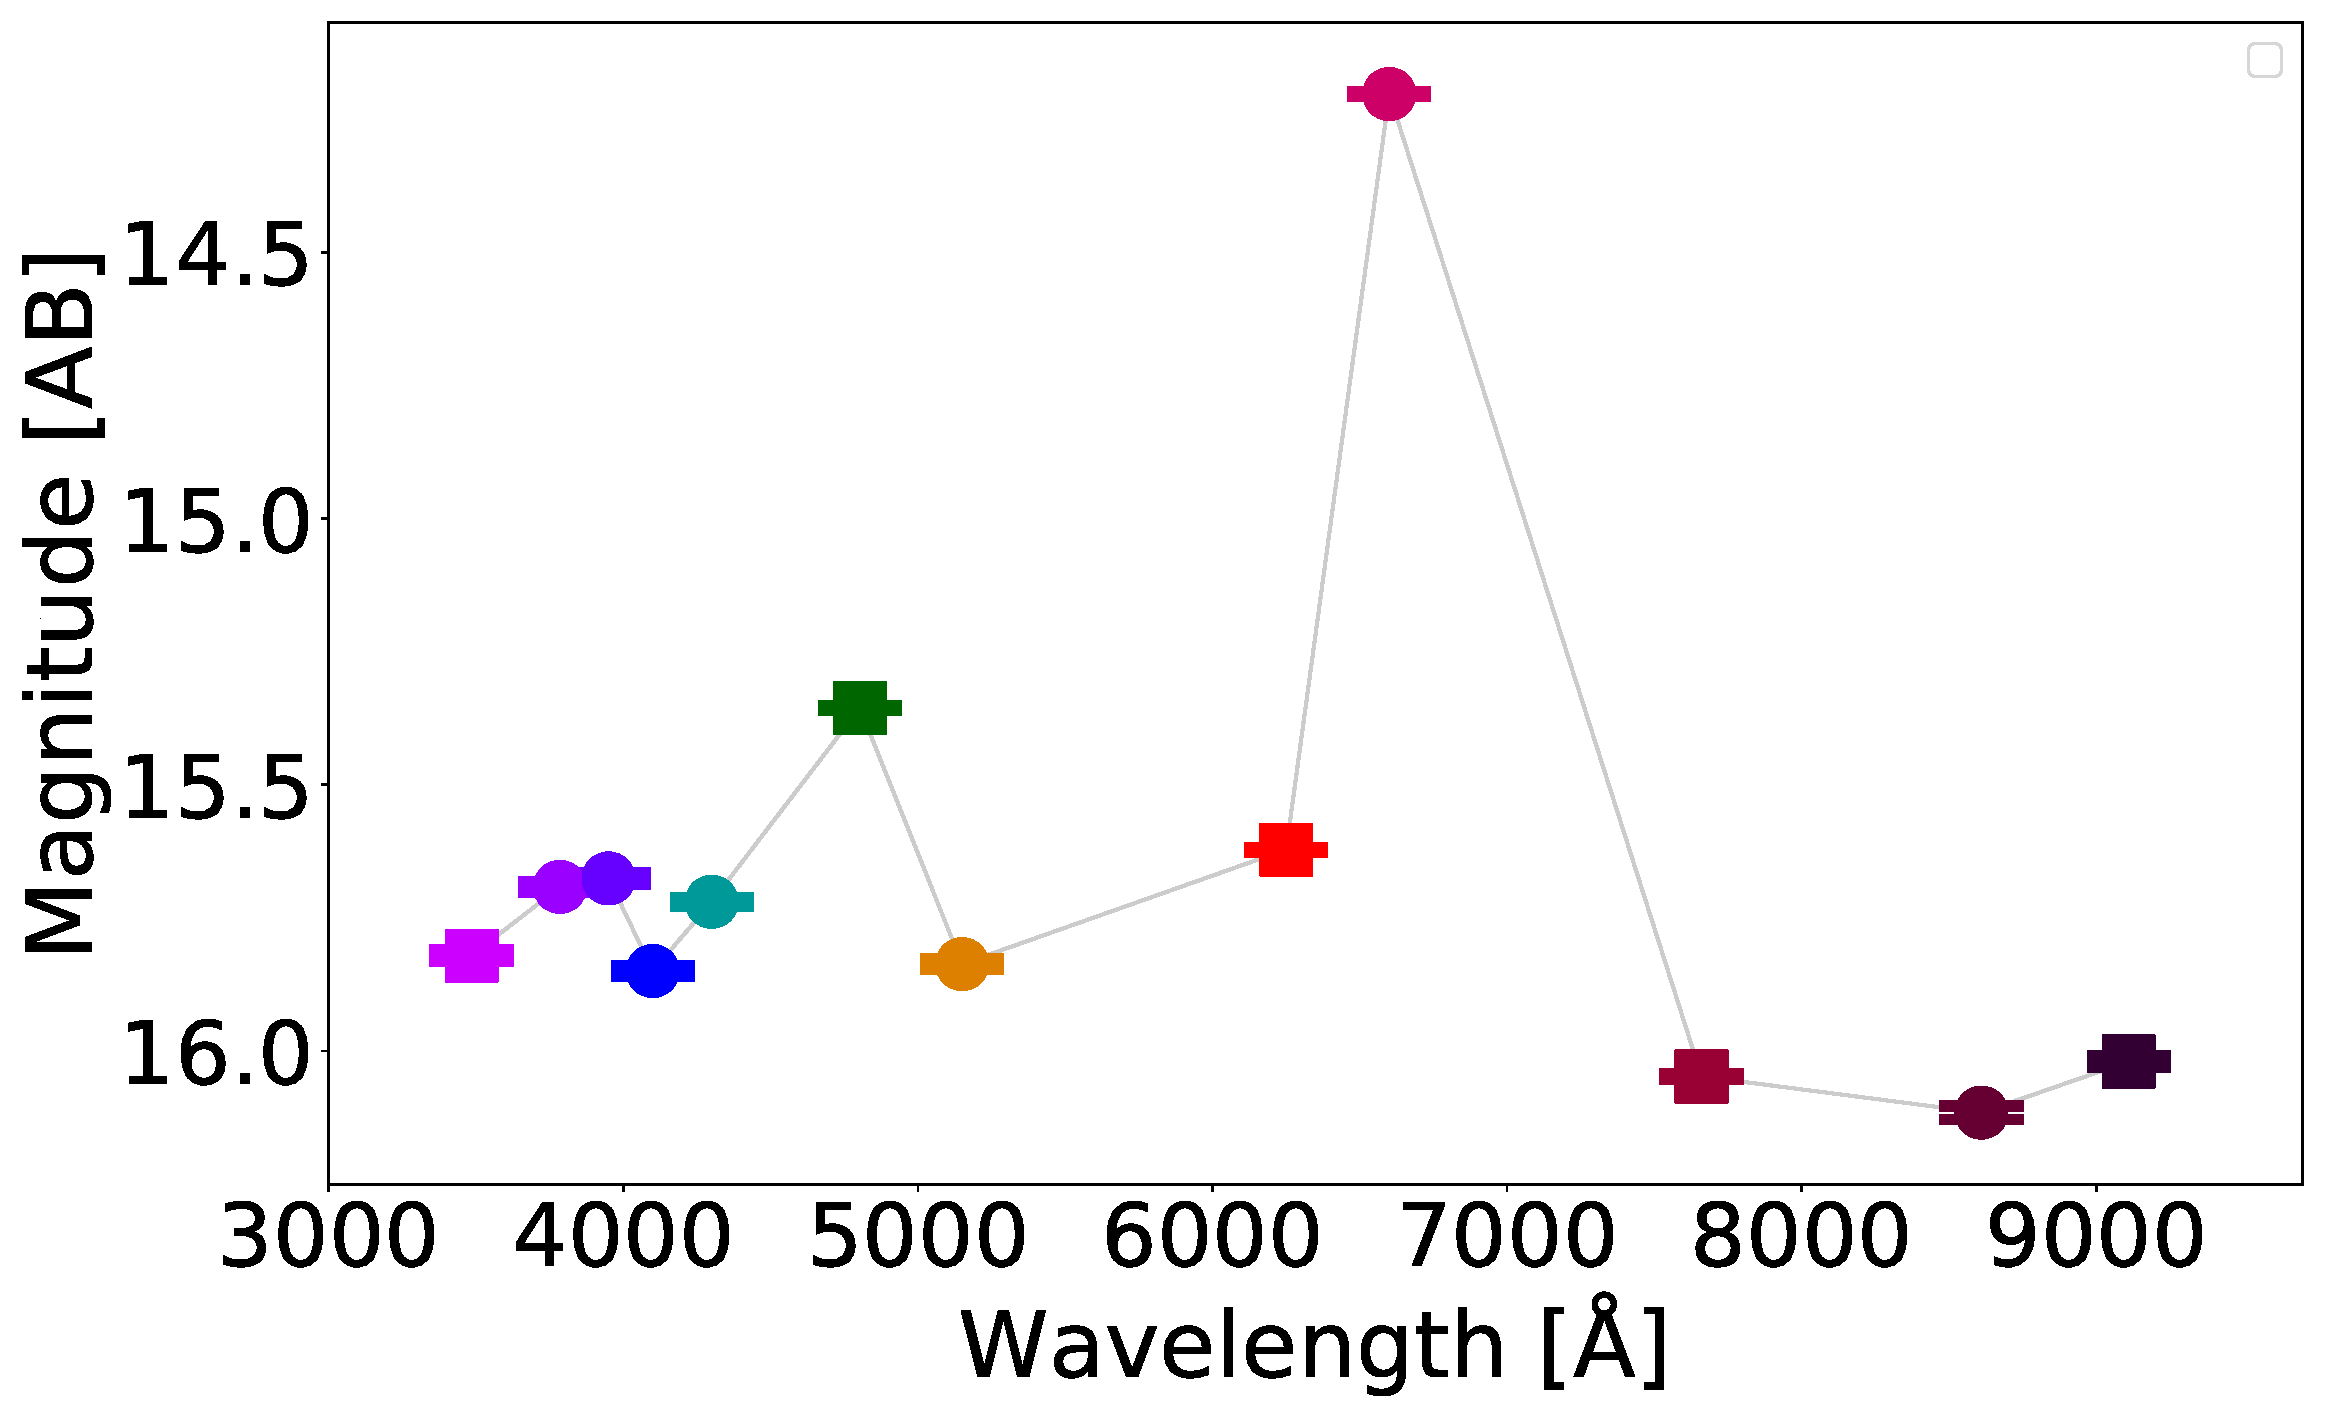
\includegraphics[width=0.3\linewidth, clip]{figs-pca/photospectrum_63391-14288-PN-pc-Halpha_emitters_threeerror-cleaning-limfilter-limcolor-flags-mask-broad_MAG_APER_6_0.pdf} & 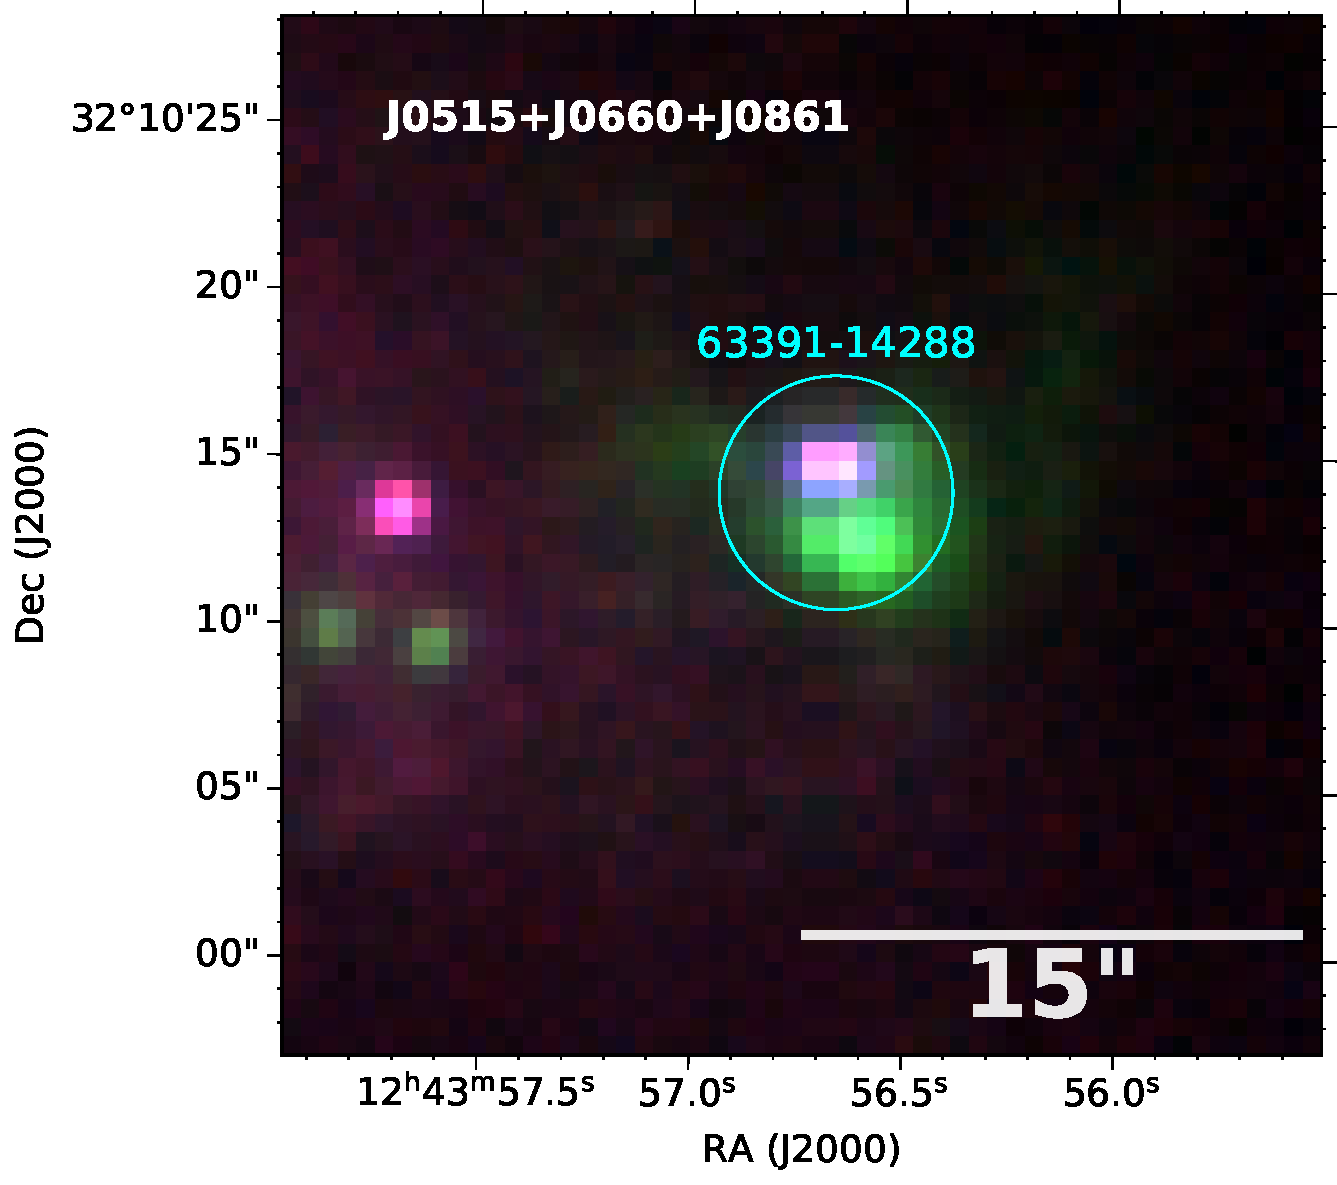
\includegraphics[width=0.3\linewidth, clip]{Field_63391/1000001-JPLUS-00899-v202006_J0861_63391-14288-RGB.pdf} & 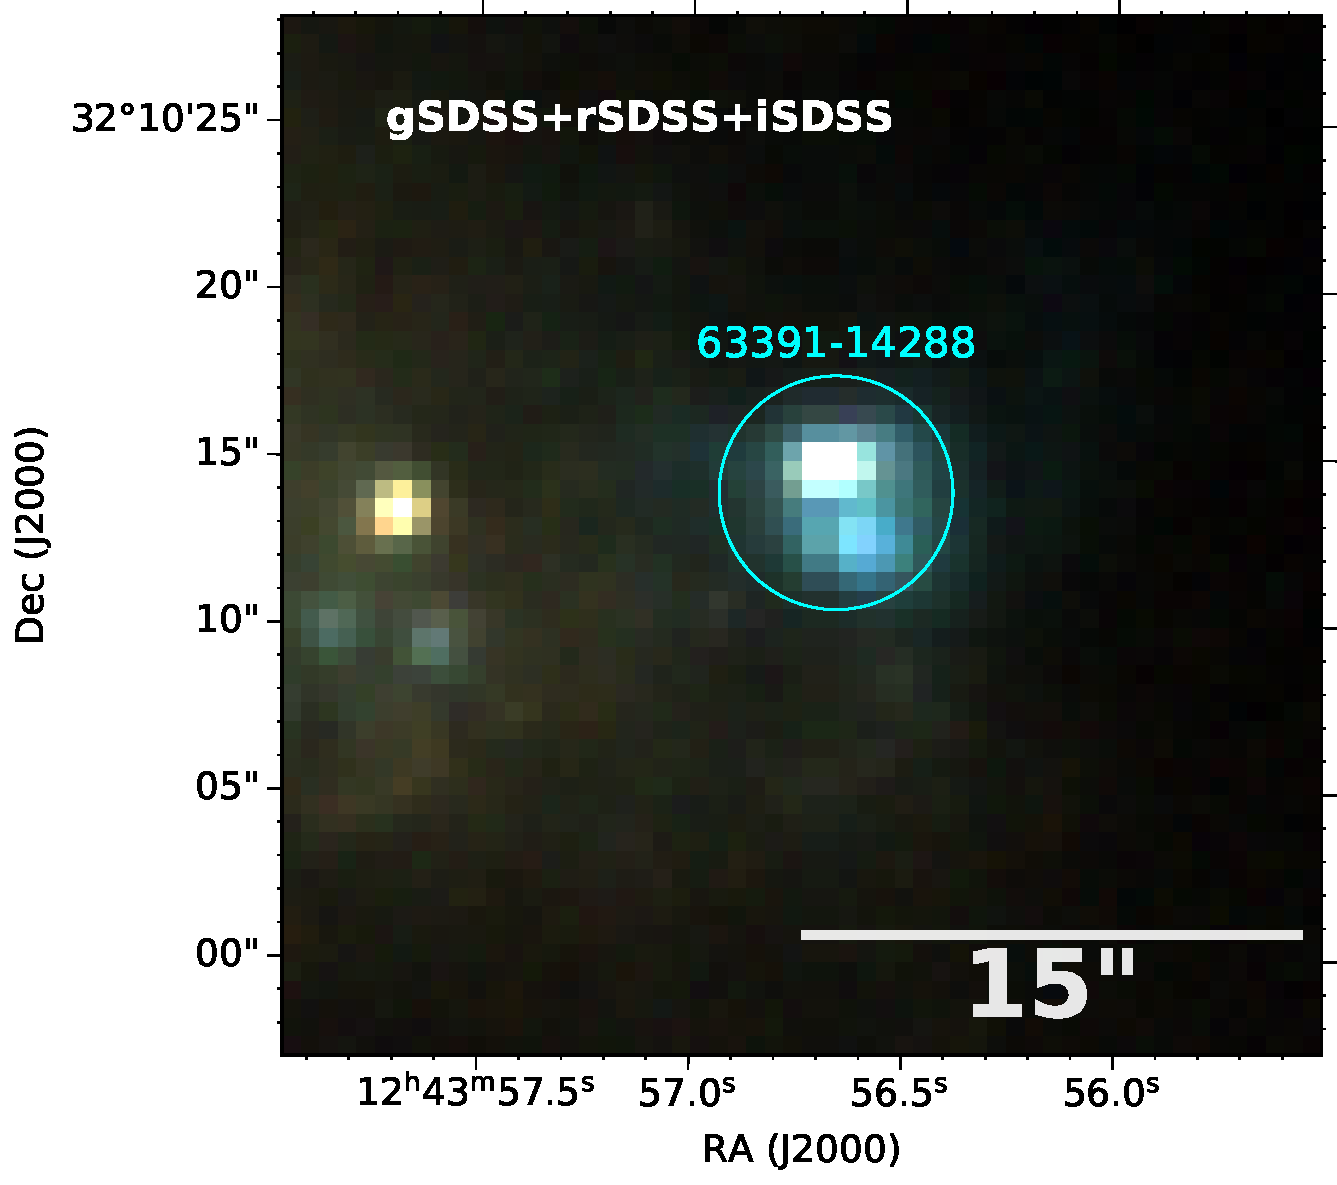
\includegraphics[width=0.3\linewidth, clip]{Field_63391/1000001-JPLUS-00899-v202006_iSDSS_63391-14288-RGB.pdf} \\
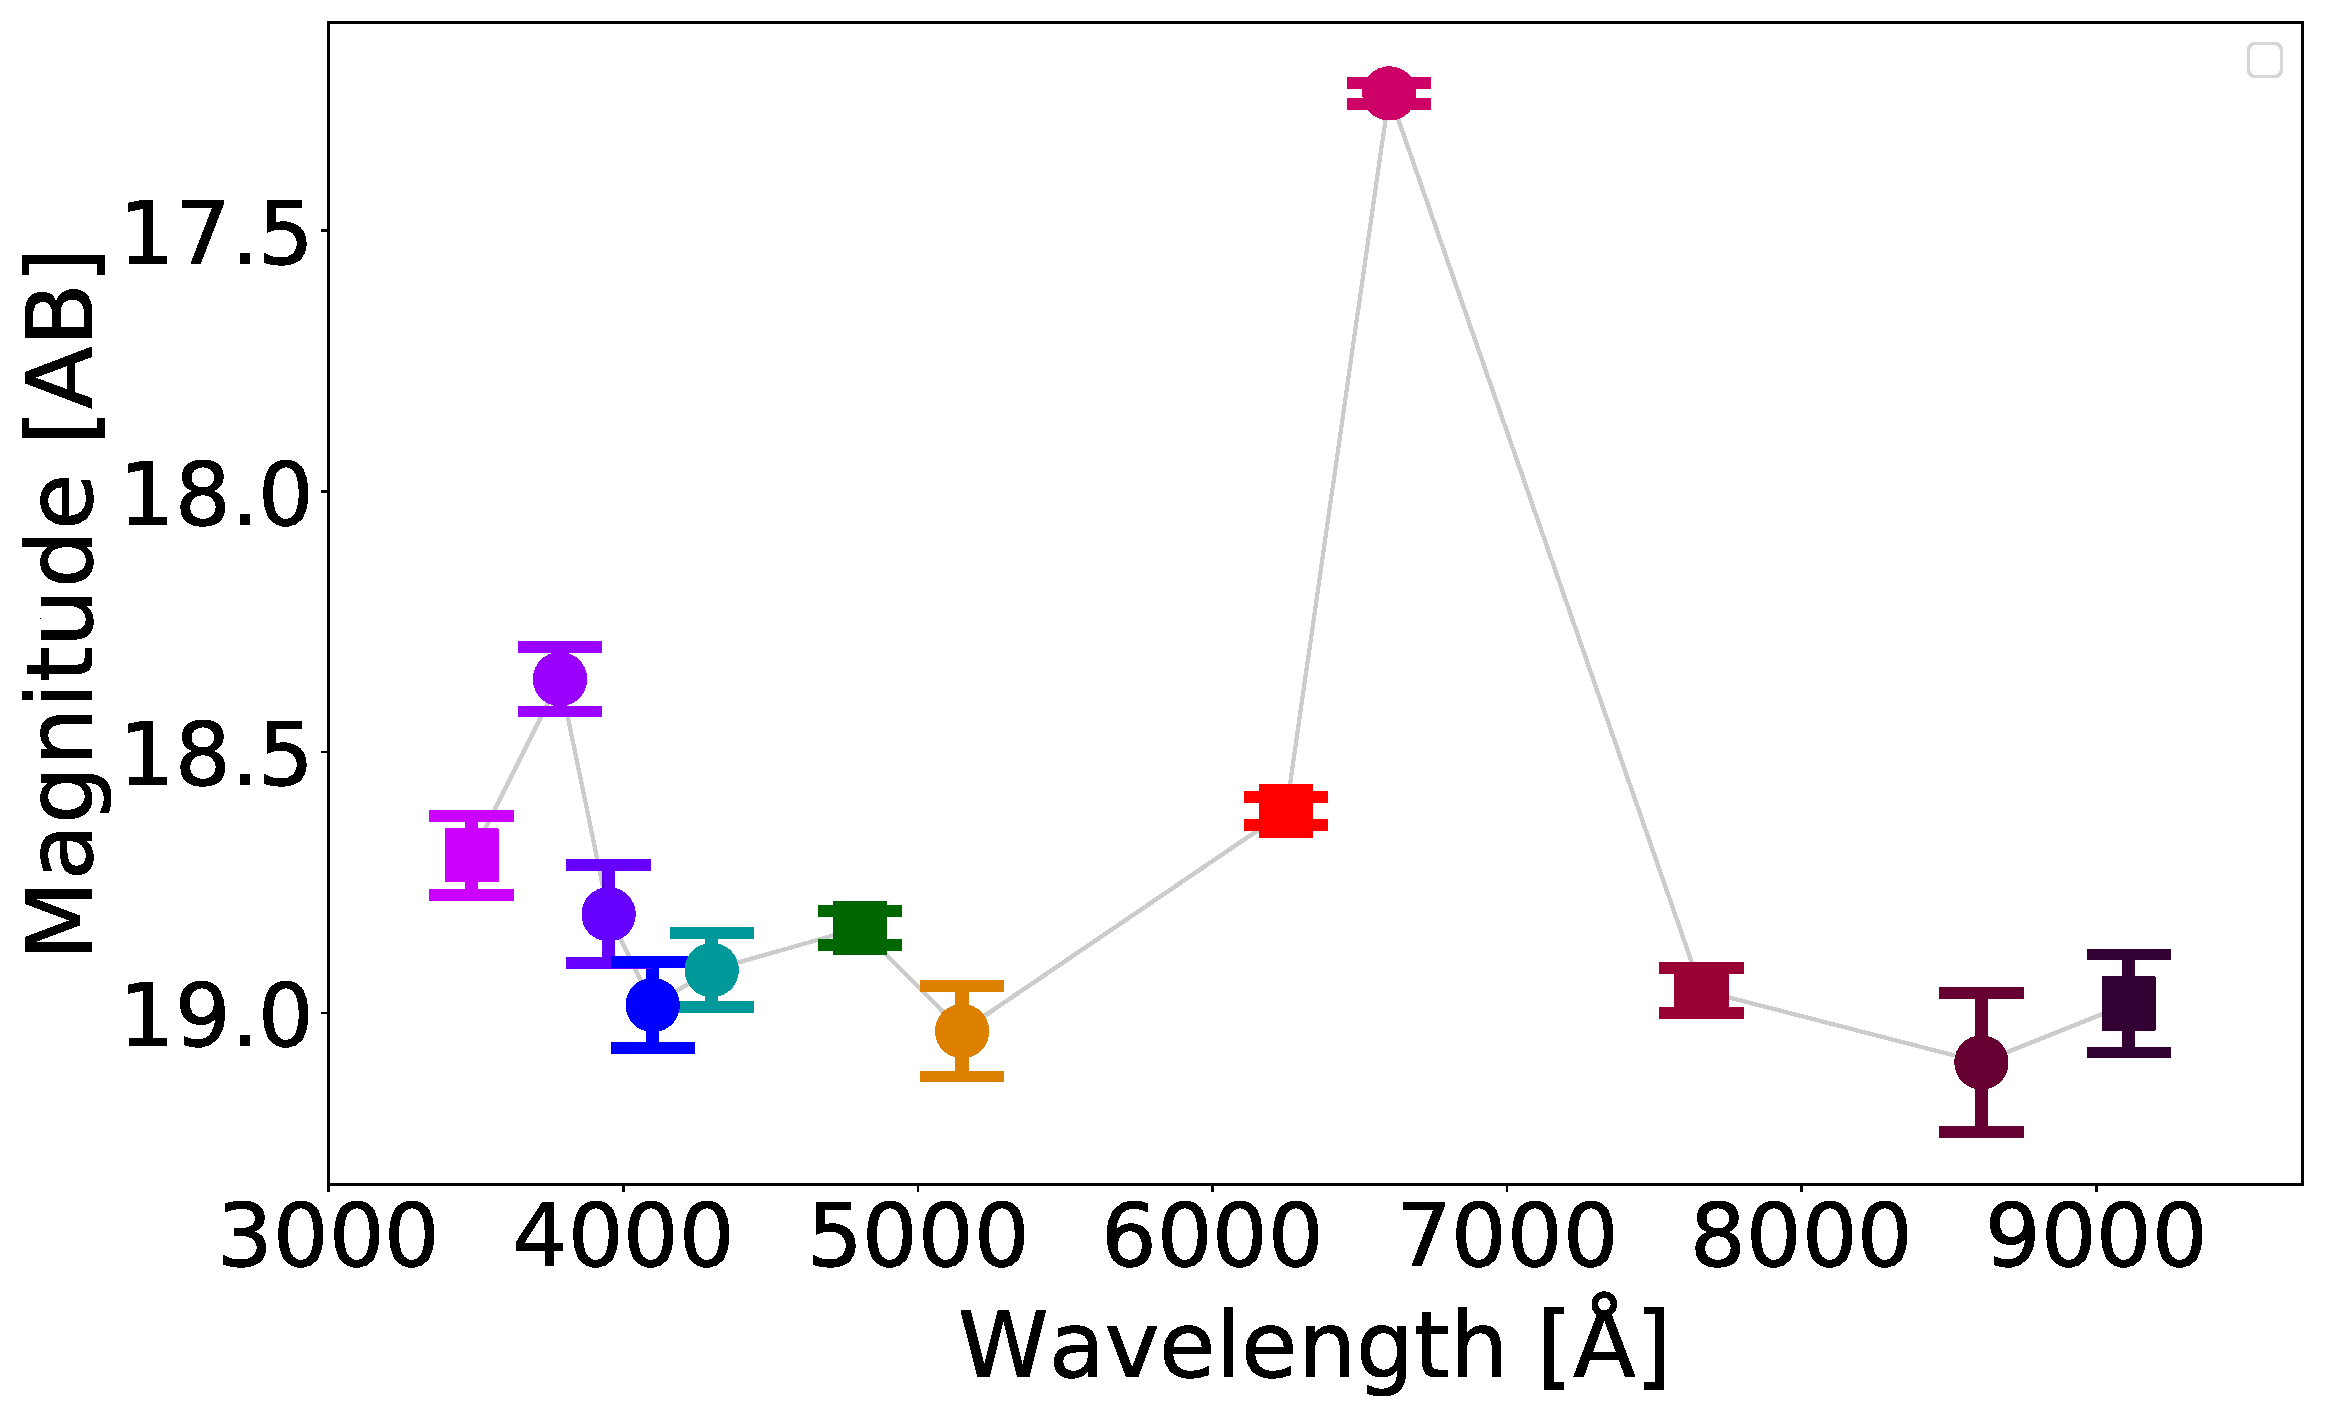
\includegraphics[width=0.3\linewidth, clip]{figs-pca/photospectrum_63728-10889-PN-pc-Halpha_emitters_threeerror-cleaning-limfilter-limcolor-flags-mask-broad_MAG_APER_6_0.pdf} & 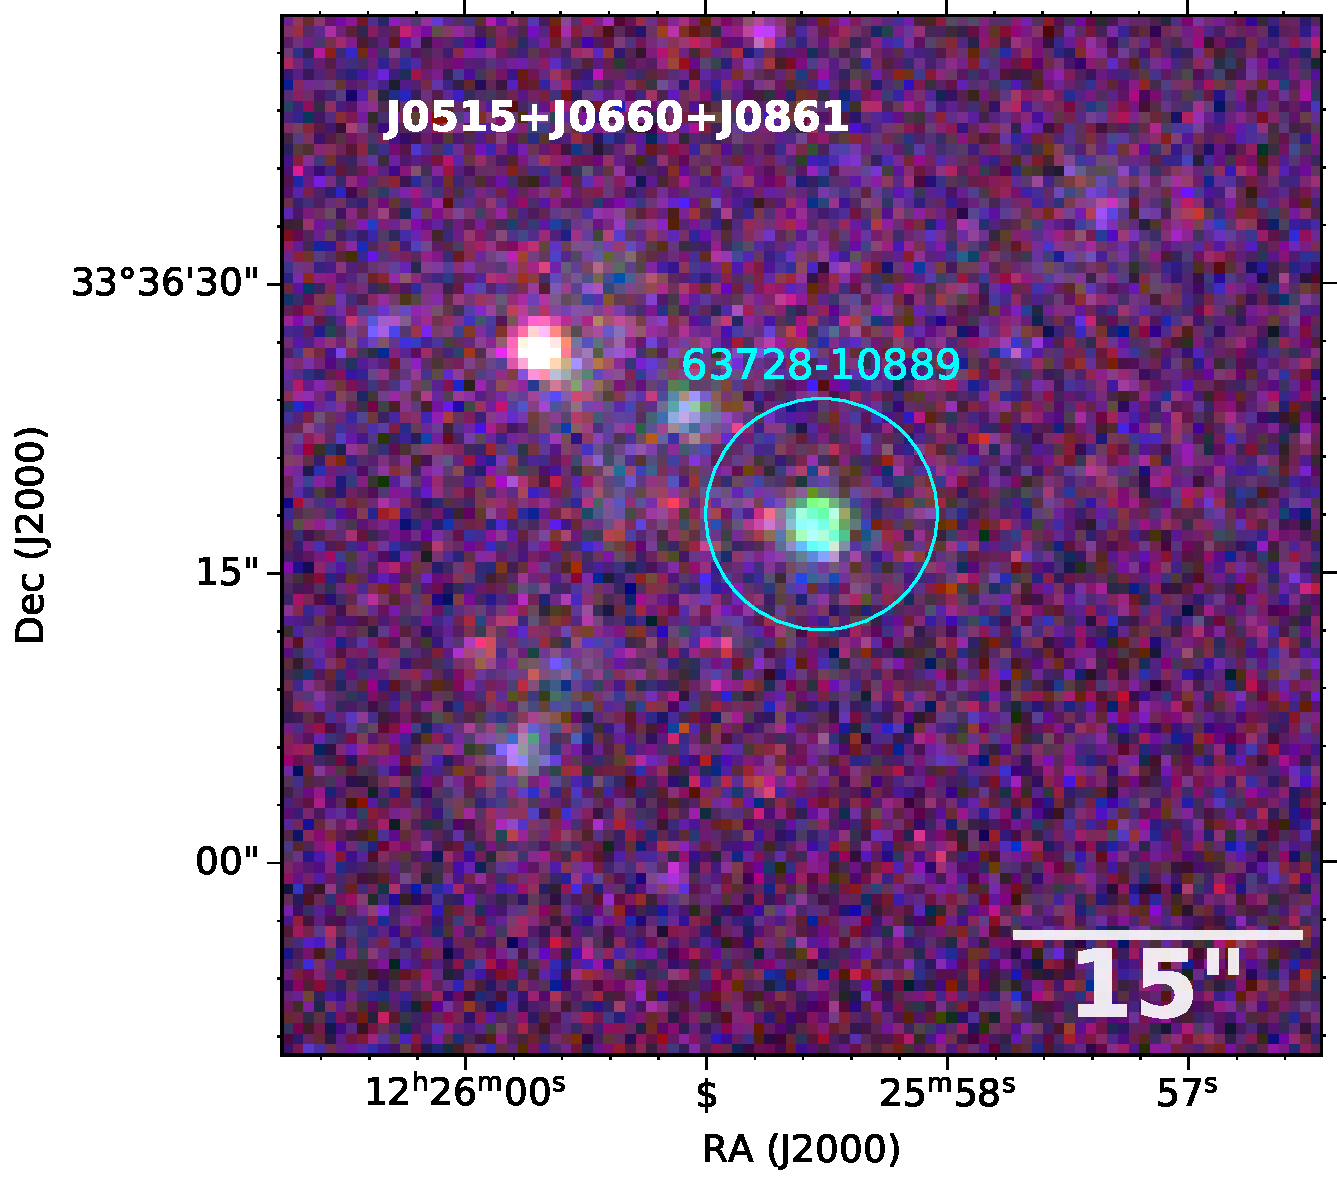
\includegraphics[width=0.3\linewidth, clip]{Field_63728/1000001-JPLUS-01007-v202006_J0861_63728-10889-RGB.pdf} & 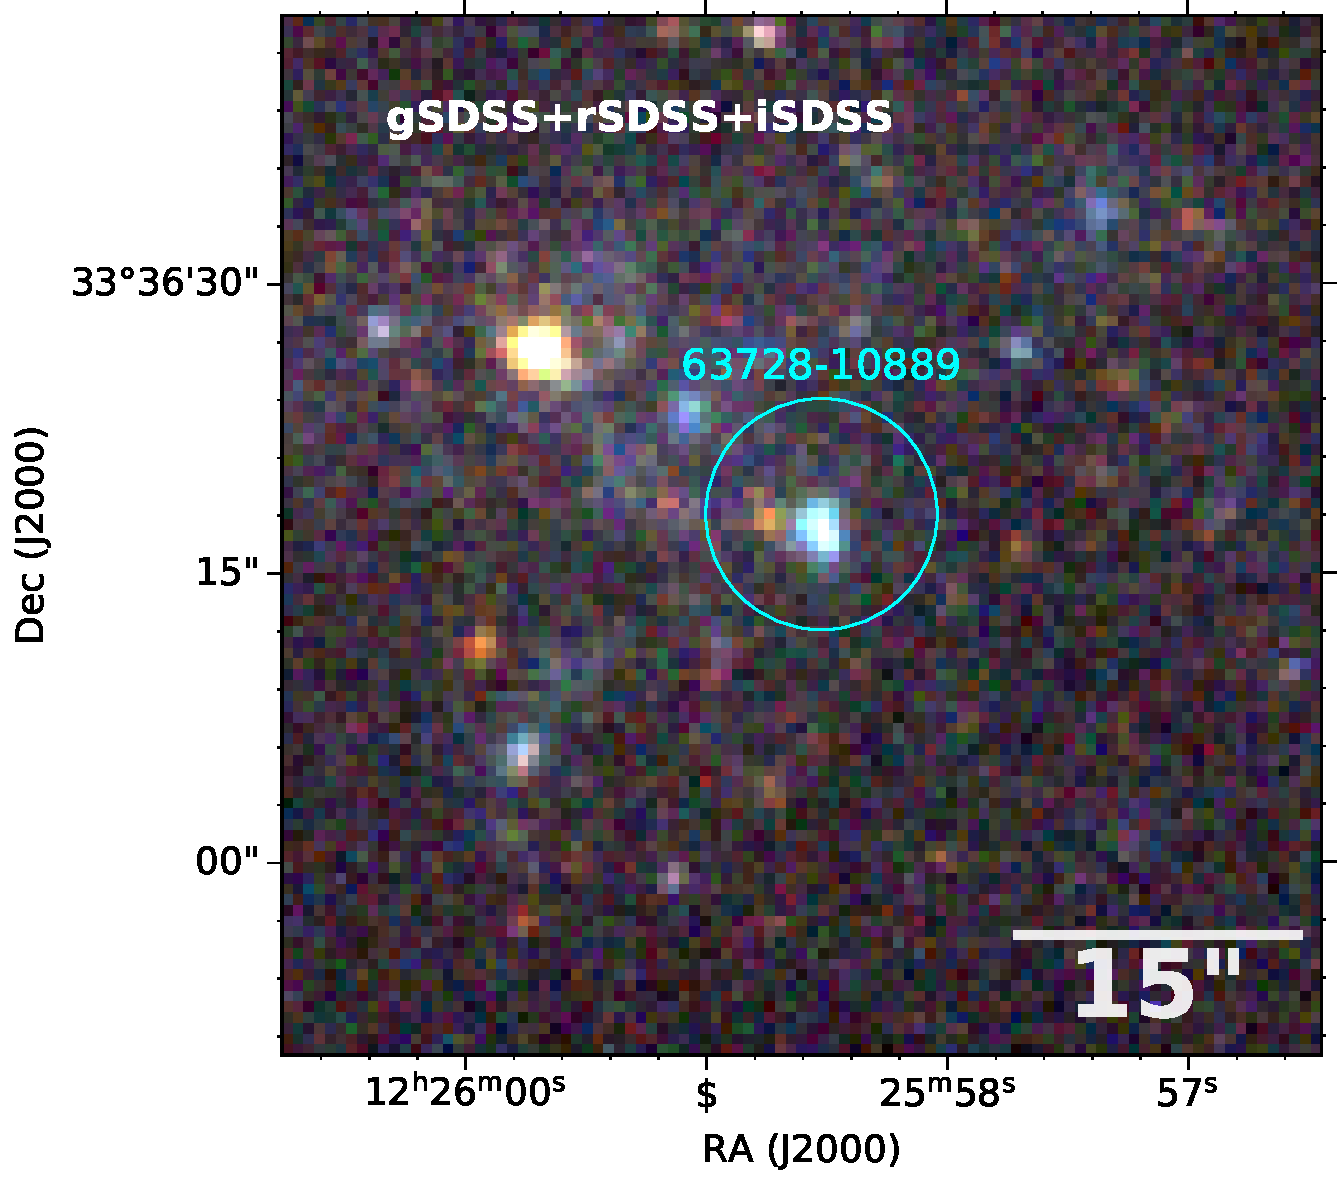
\includegraphics[width=0.3\linewidth, clip]{Field_63728/1000001-JPLUS-01007-v202006_iSDSS_63728-10889-RGB.pdf} \\
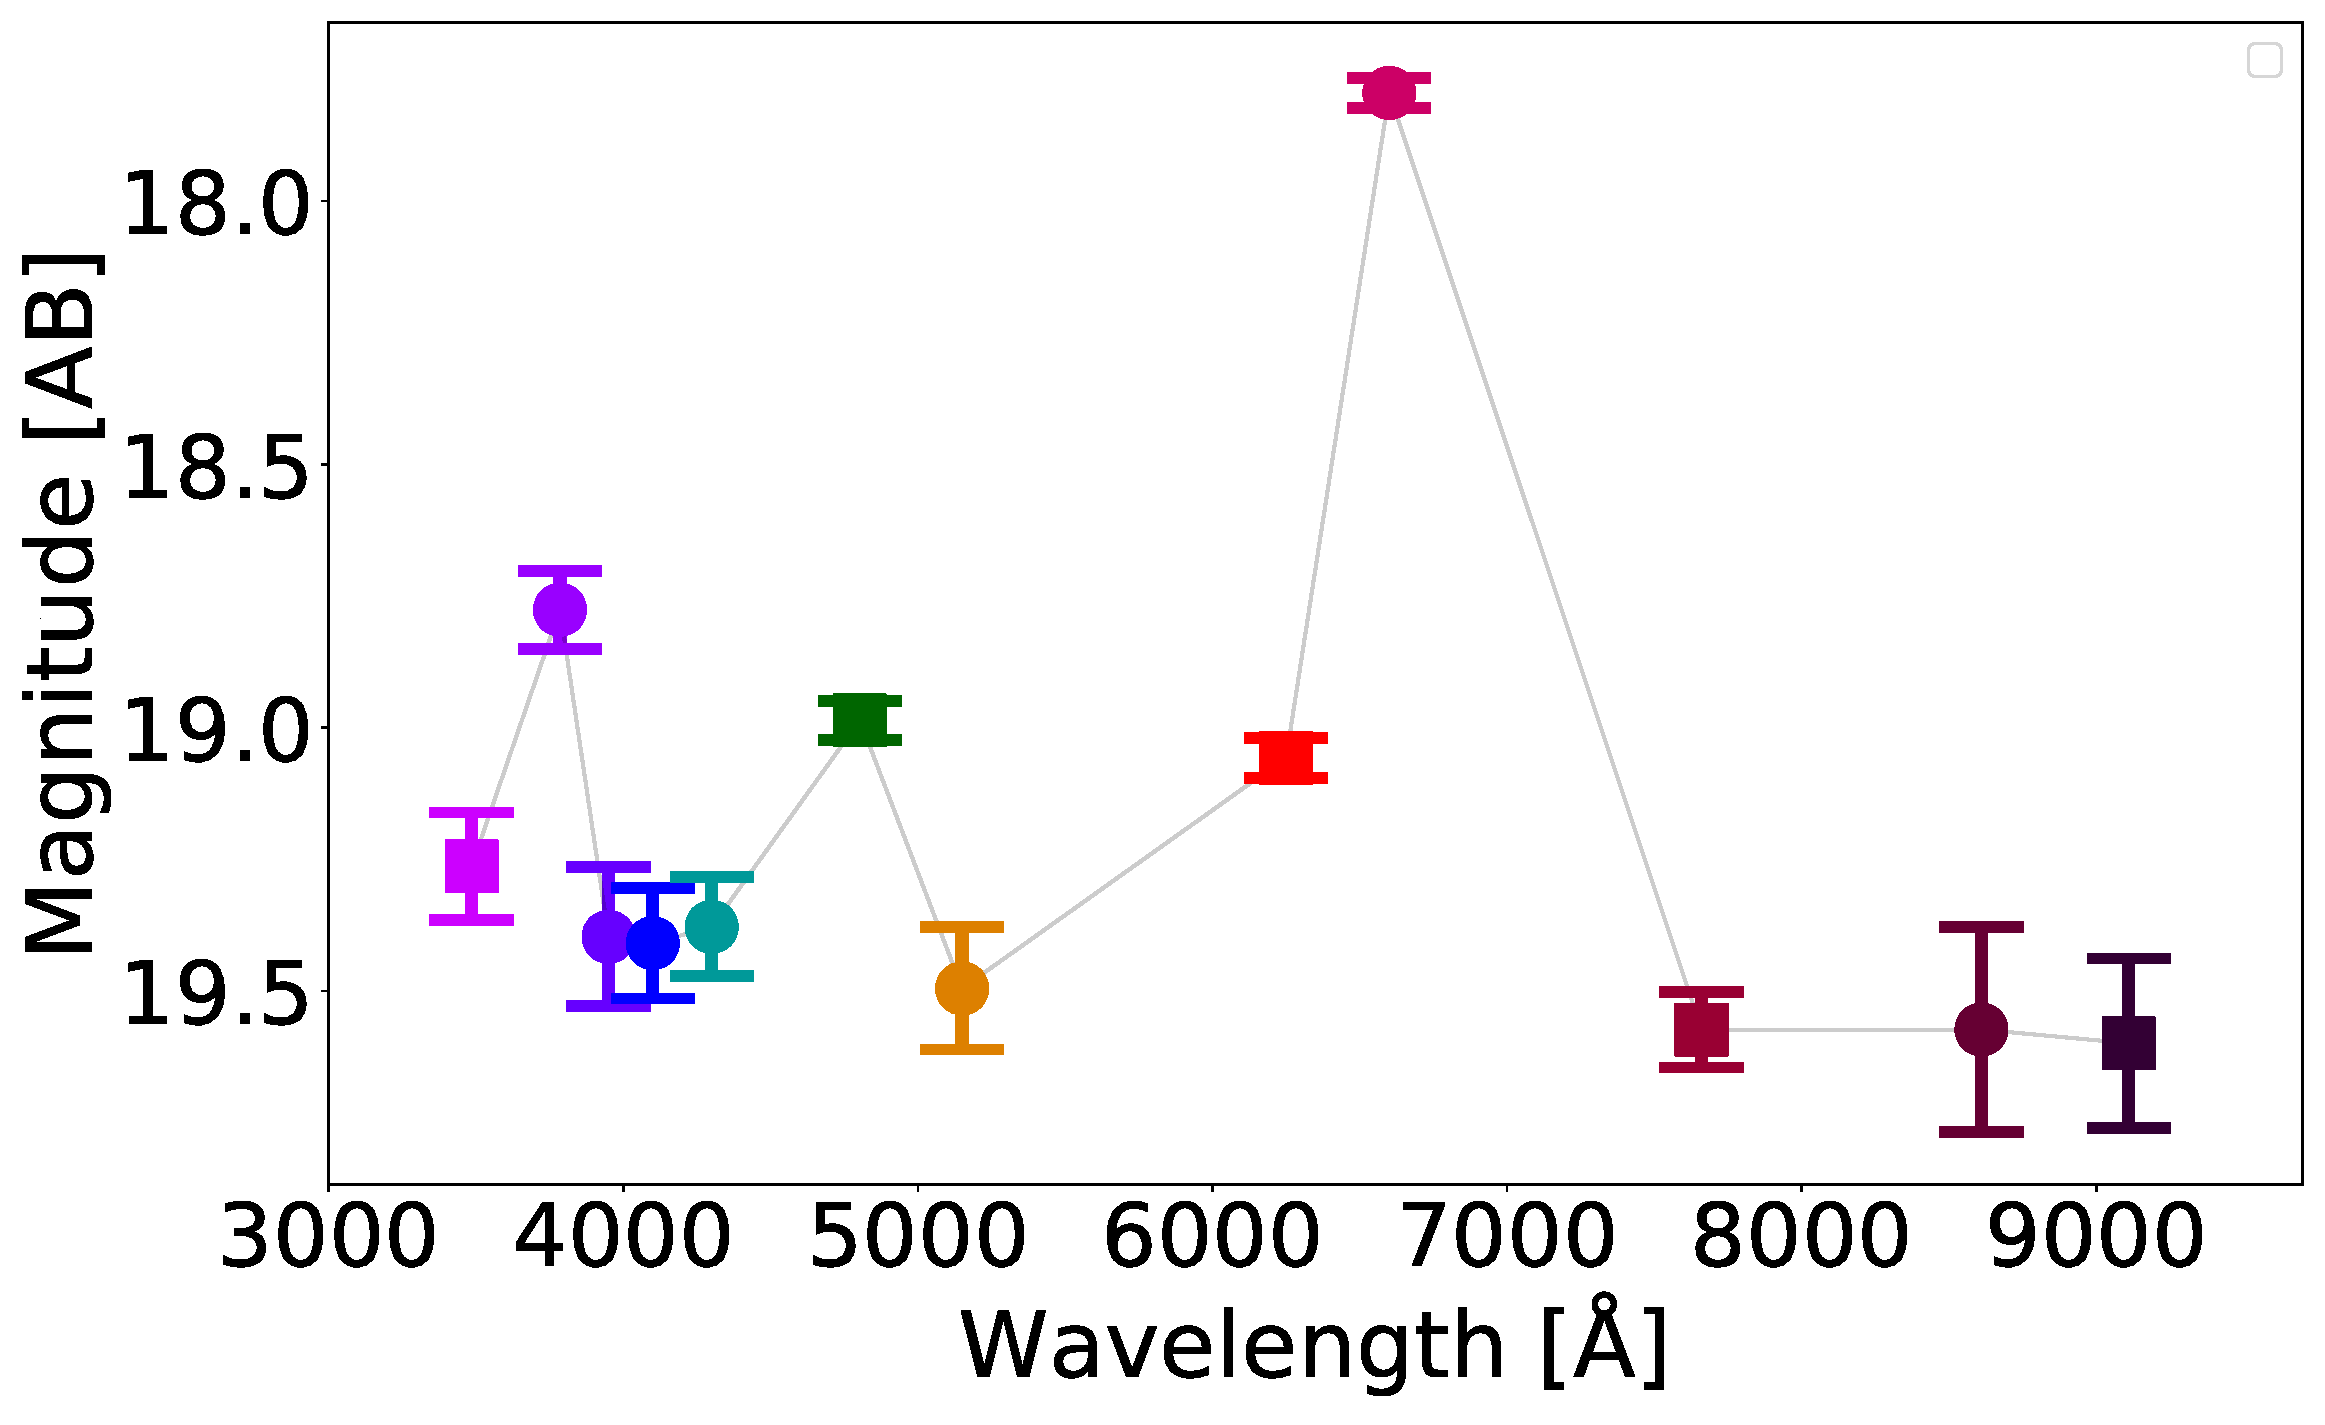
\includegraphics[width=0.3\linewidth, clip]{figs-pca/photospectrum_63728-15748-PN-pc-Halpha_emitters_threeerror-cleaning-limfilter-limcolor-flags-mask-broad_MAG_APER_6_0.pdf} & 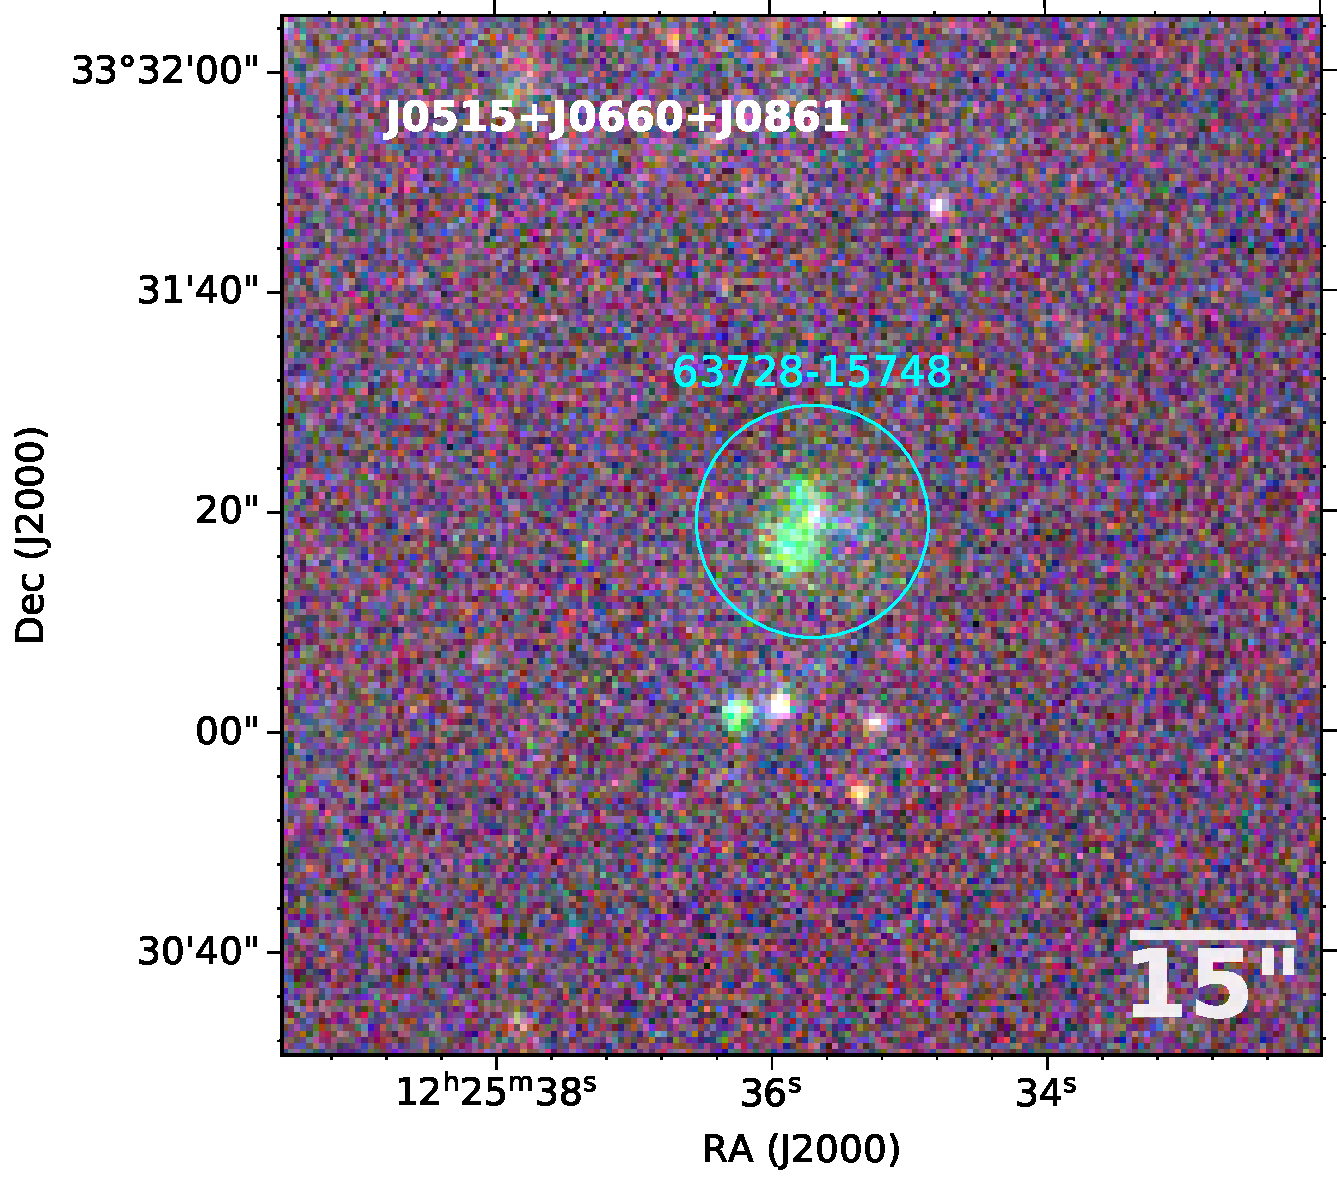
\includegraphics[width=0.3\linewidth, clip]{Field_63728/1000001-JPLUS-01007-v202006_J0861_63728-15748-RGB.pdf} & 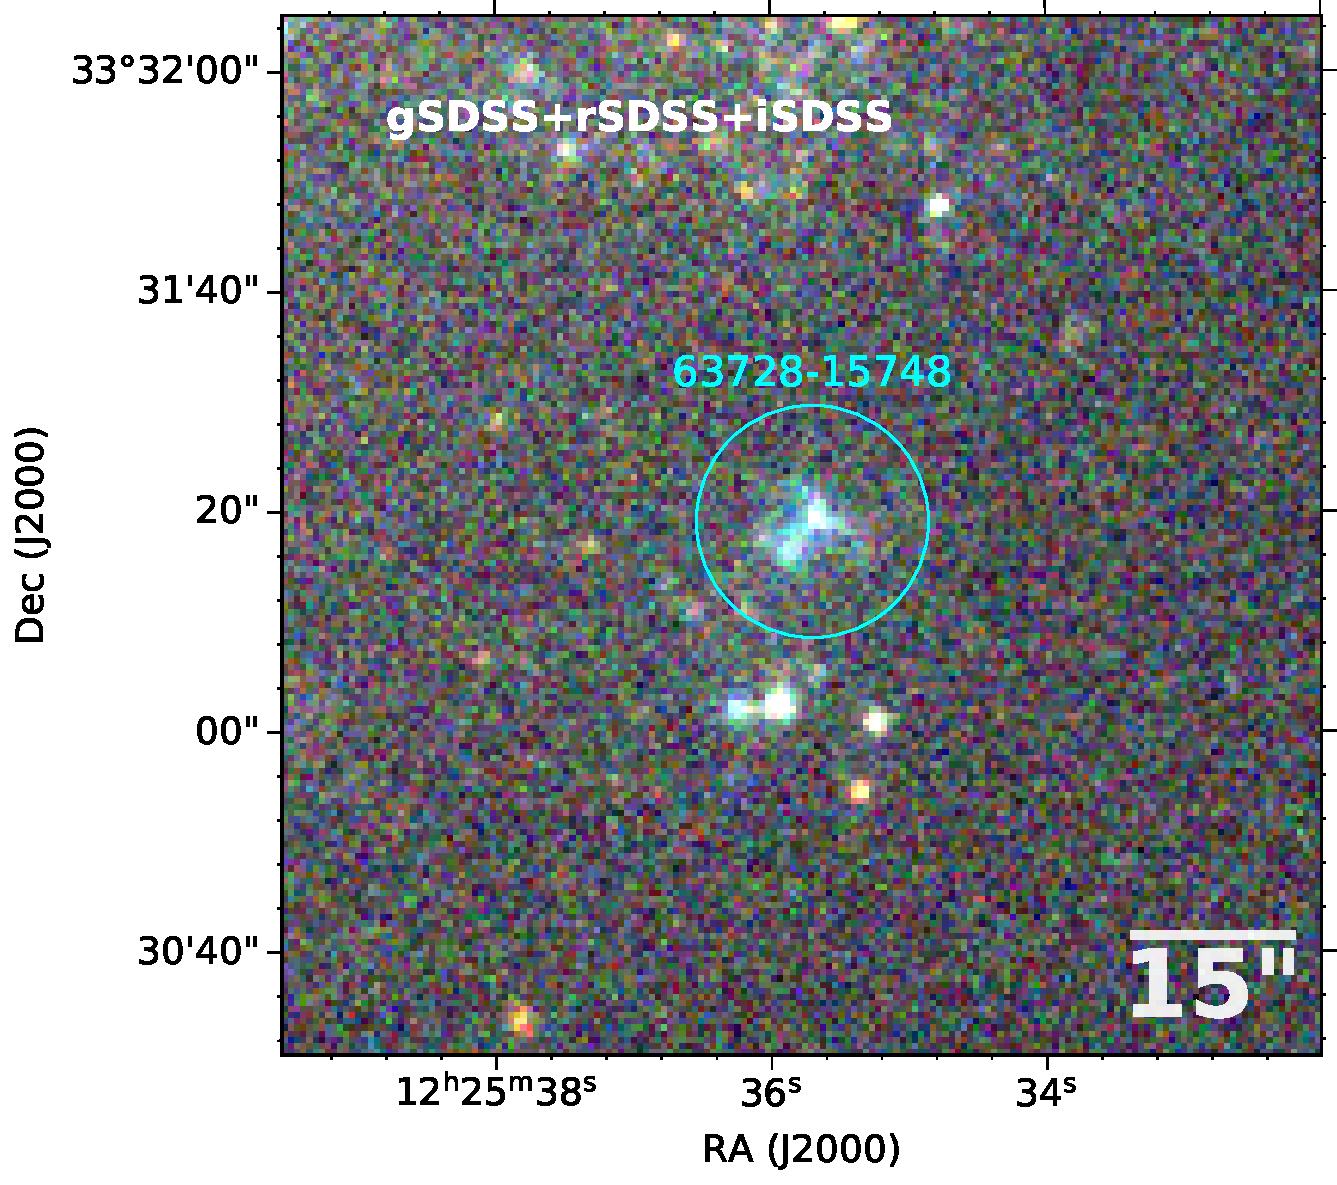
\includegraphics[width=0.3\linewidth, clip]{Field_63728/1000001-JPLUS-01007-v202006_iSDSS_63728-15748-RGB.pdf} \\
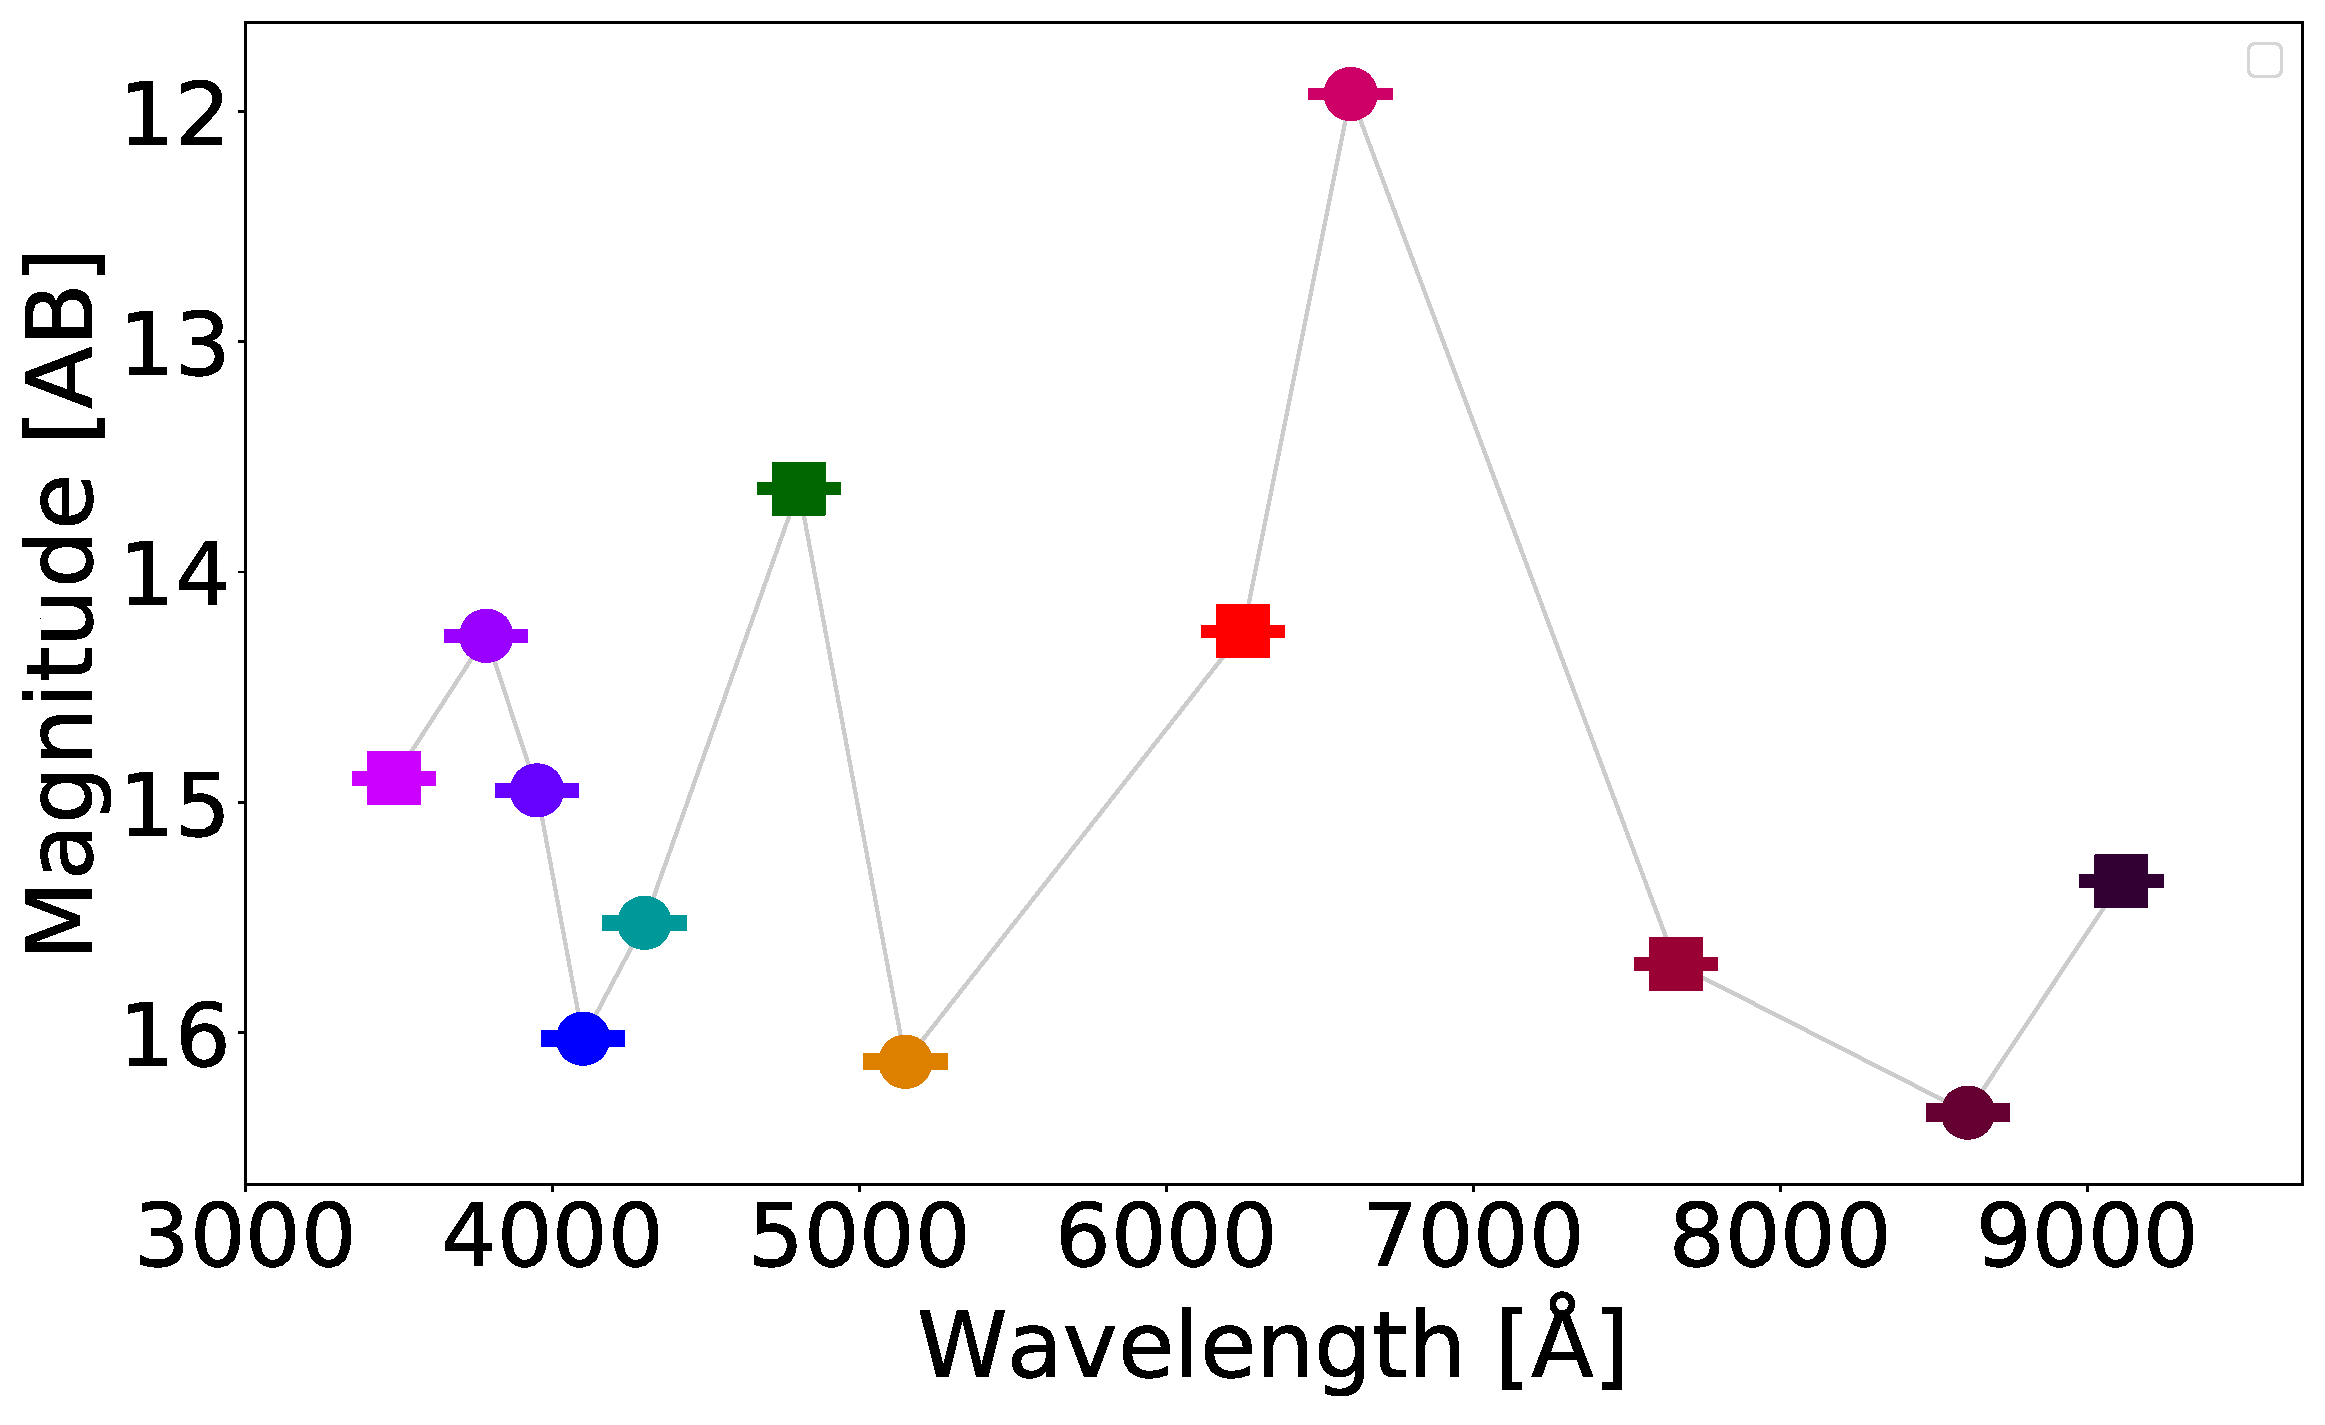
\includegraphics[width=0.3\linewidth, clip]{figs-pca/photospectrum_63864-47481-PN-pc-Halpha_emitters_threeerror-cleaning-limfilter-limcolor-flags-mask-broad_MAG_APER_6_0.pdf} & 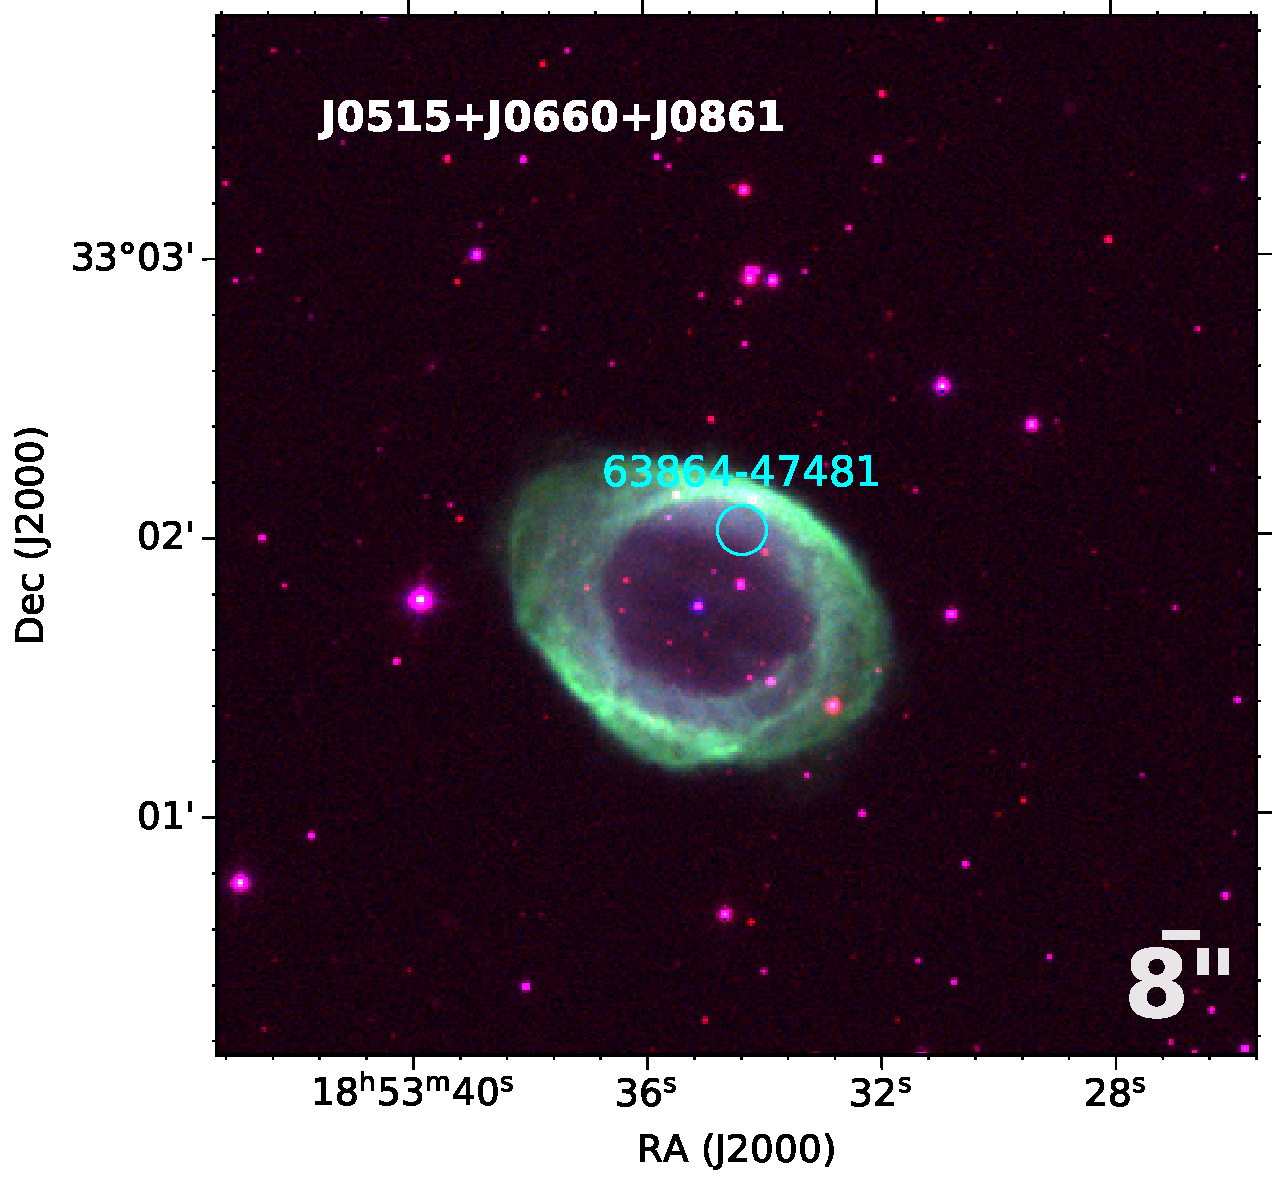
\includegraphics[width=0.3\linewidth, clip]{Field_63864/1000001-JPLUS-01066-v202006_J0861_63864-47481-RGB.pdf} & 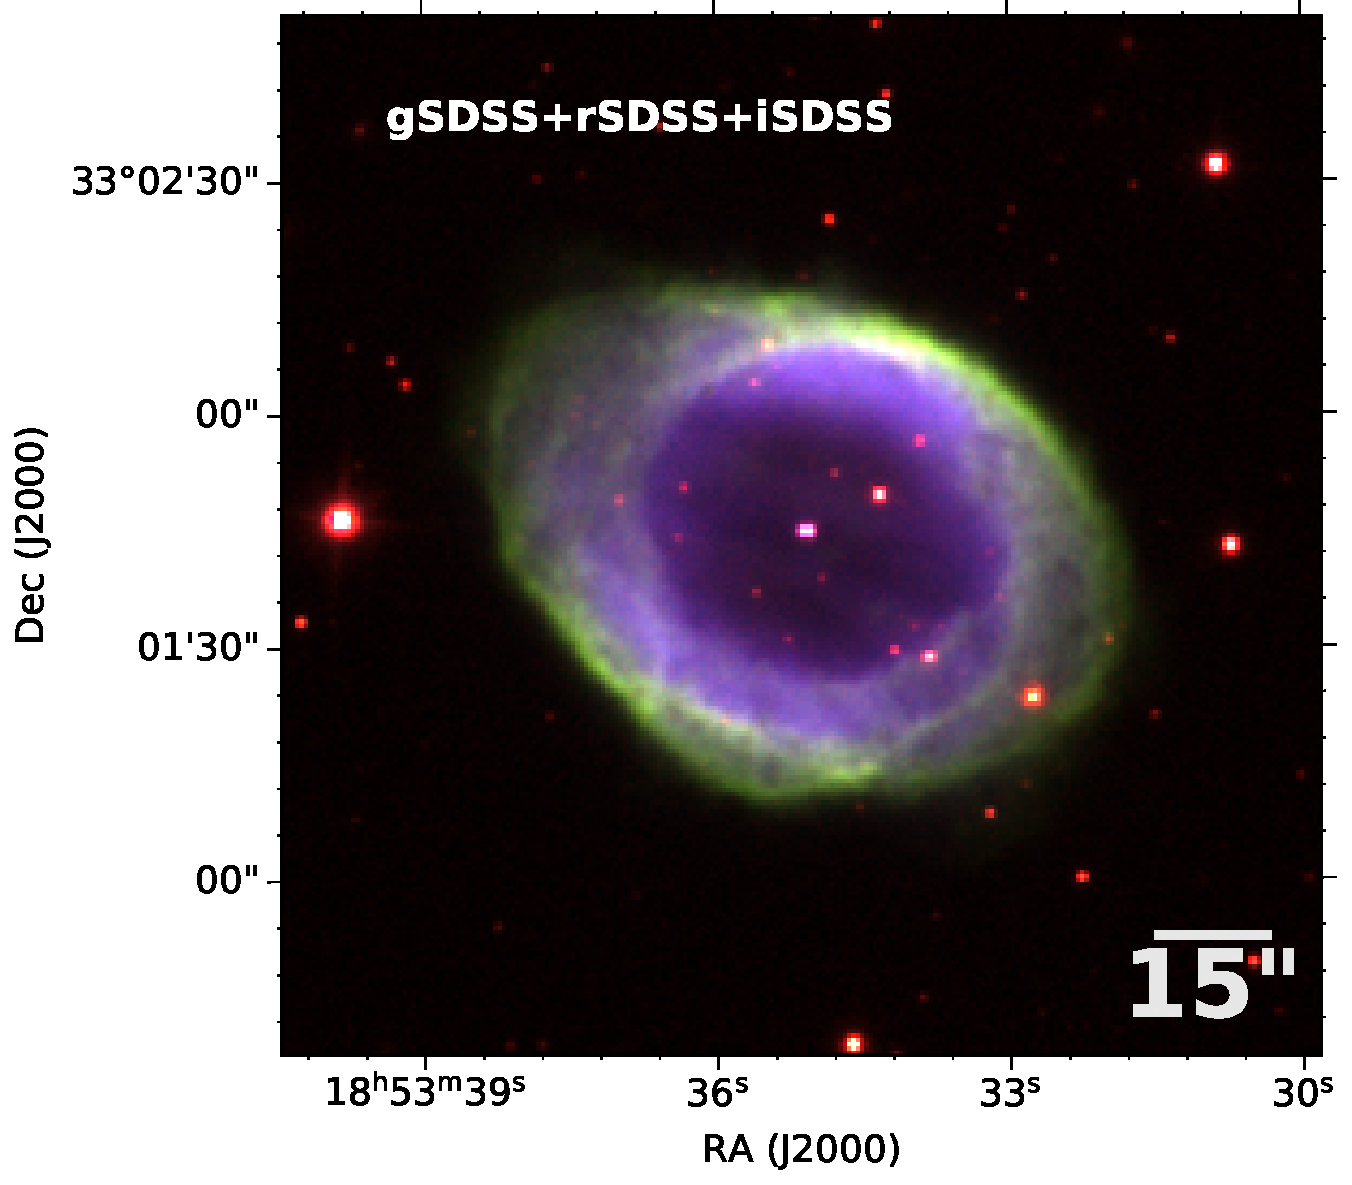
\includegraphics[width=0.3\linewidth, clip]{Field_63864/1000001-JPLUS-01066-v202006_iSDSS_63864-47481-RGB.pdf} \\
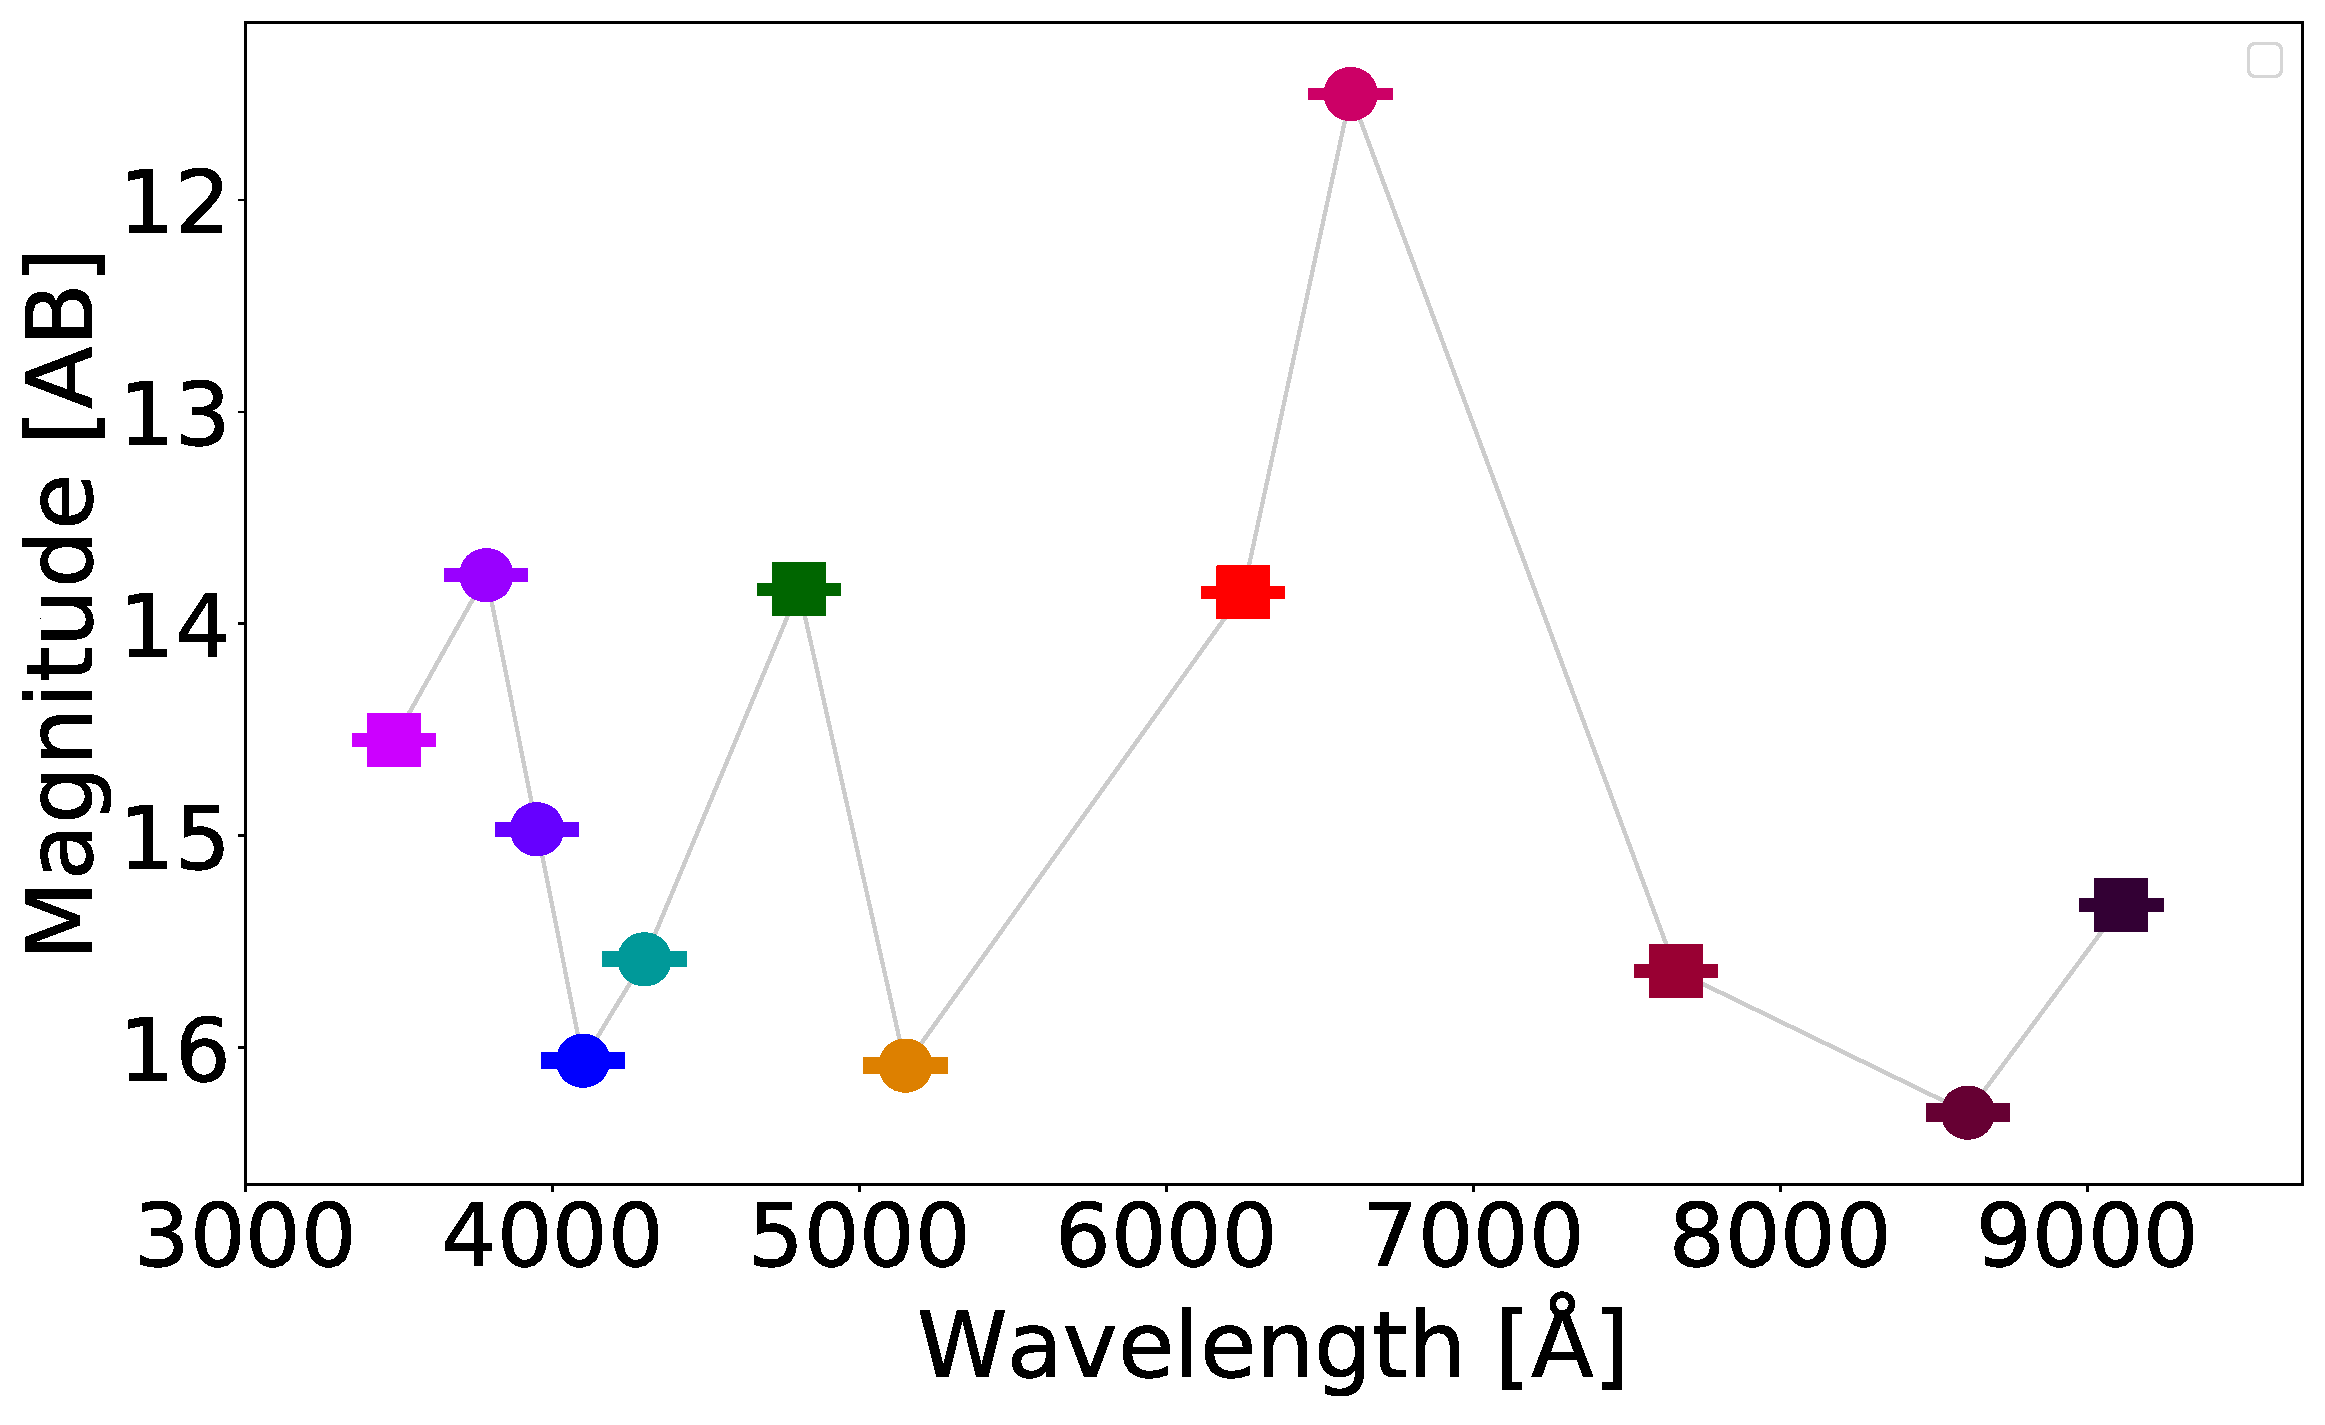
\includegraphics[width=0.3\linewidth, clip]{figs-pca/photospectrum_63864-51786-PN-pc-Halpha_emitters_threeerror-cleaning-limfilter-limcolor-flags-mask-broad_MAG_APER_6_0.pdf} & 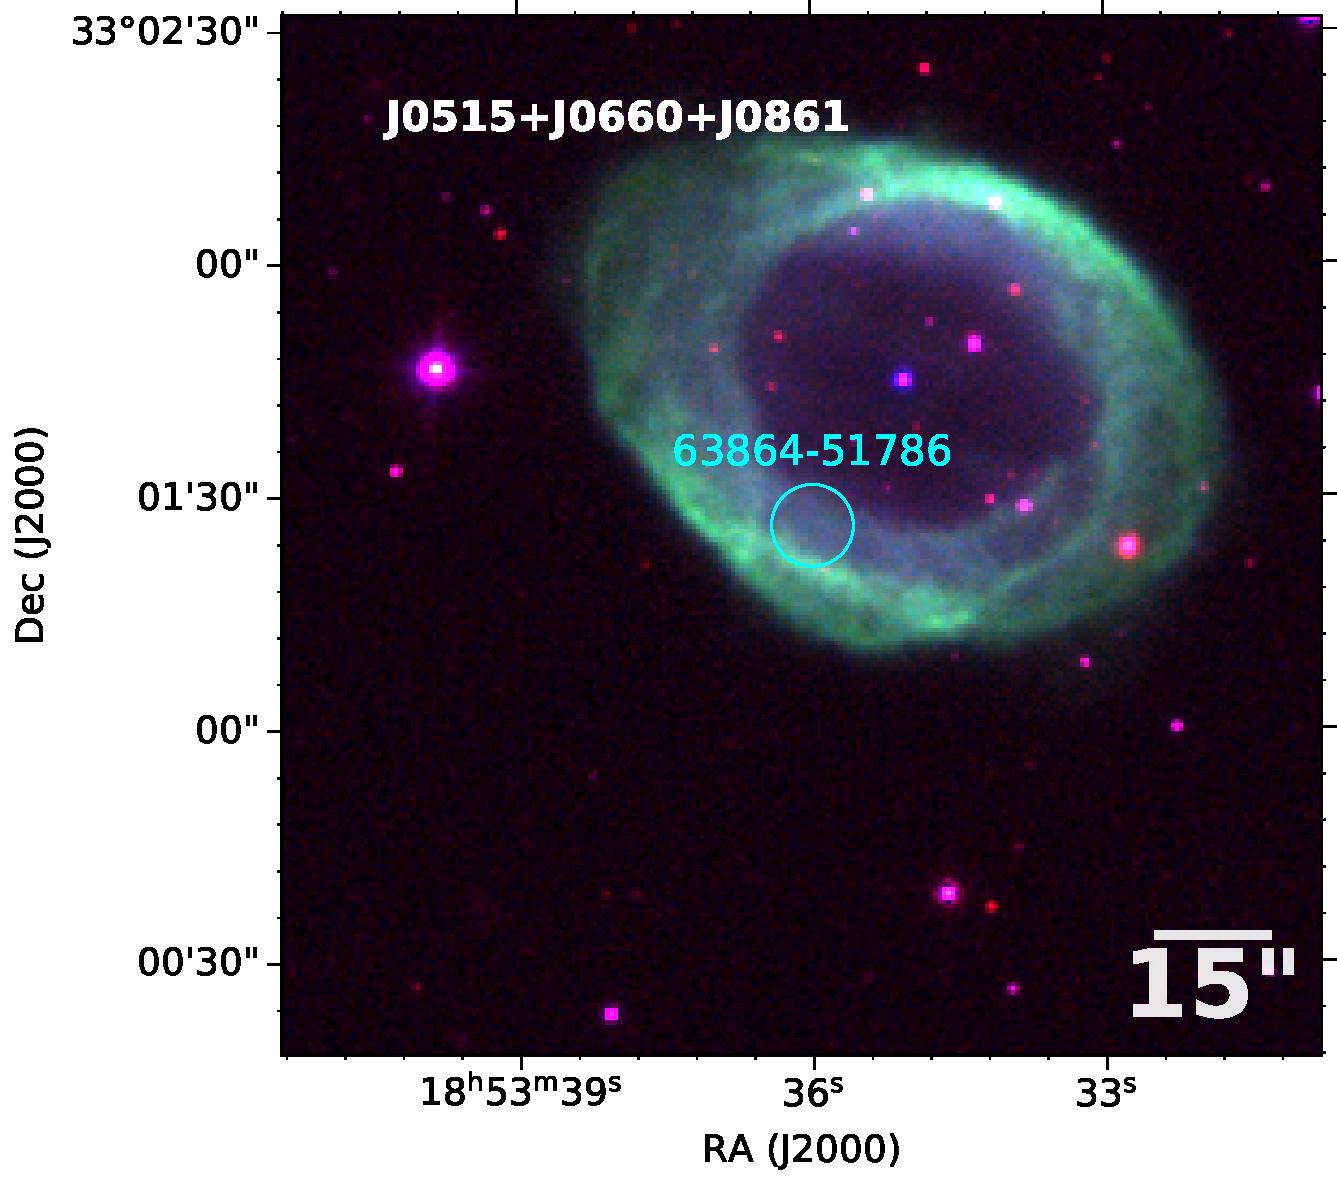
\includegraphics[width=0.3\linewidth, clip]{Field_63864/1000001-JPLUS-01066-v202006_J0861_63864-51786-RGB.pdf} & 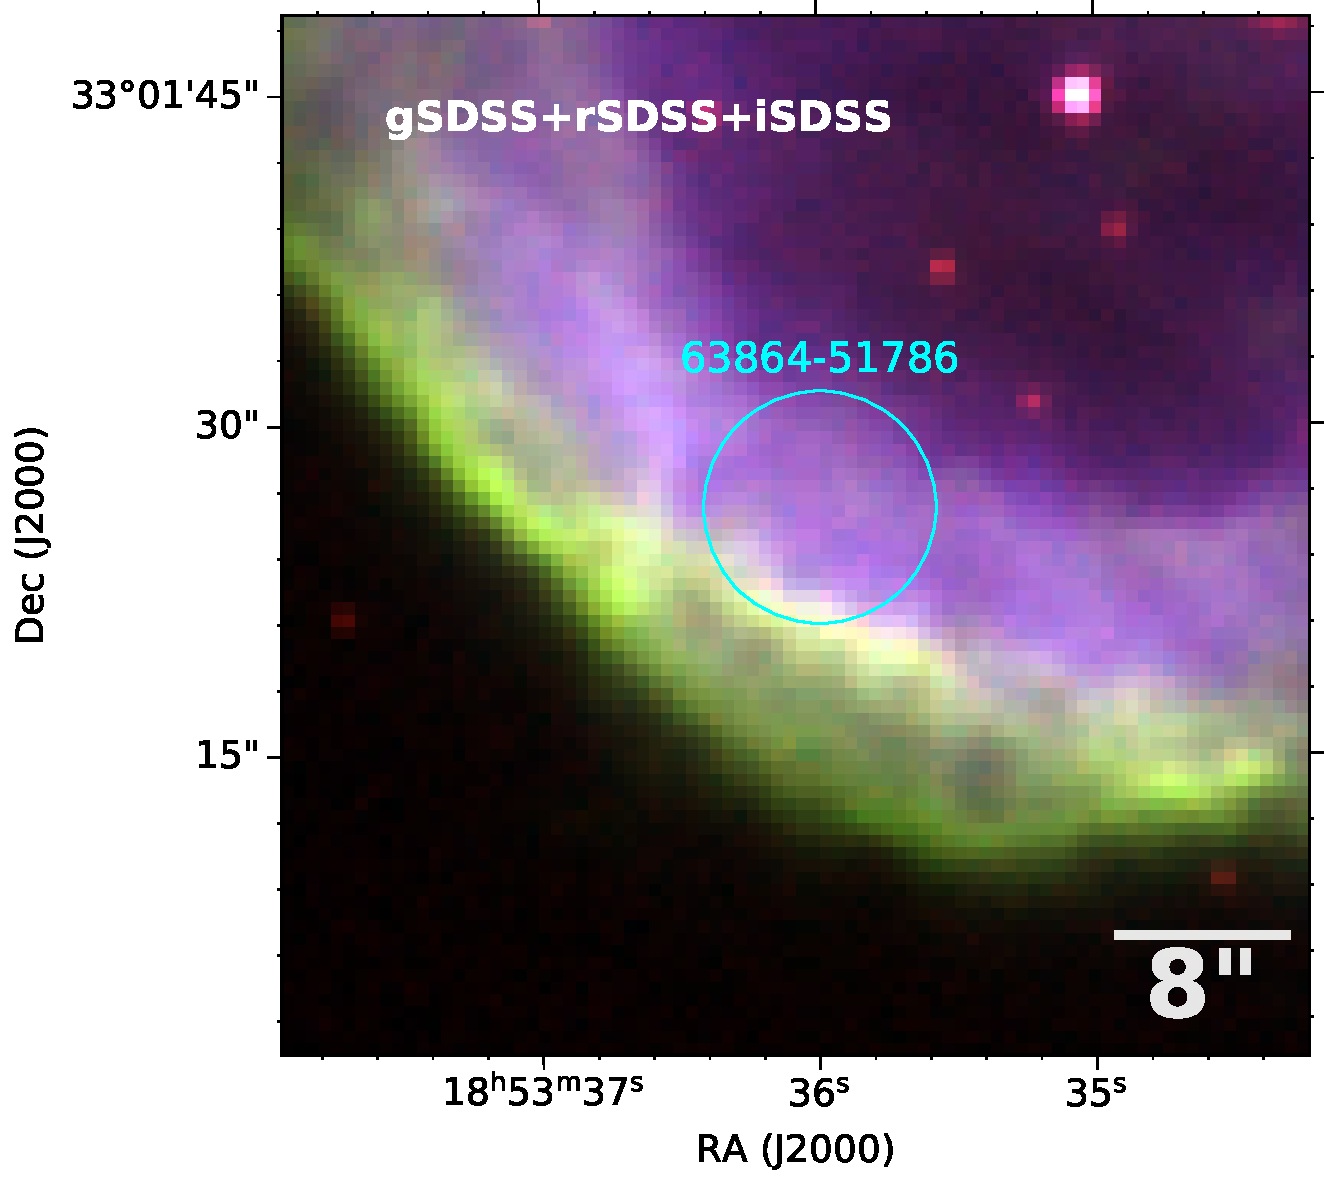
\includegraphics[width=0.3\linewidth, clip]{Field_63864/1000001-JPLUS-01066-v202006_iSDSS_63864-51786-RGB.pdf} \\
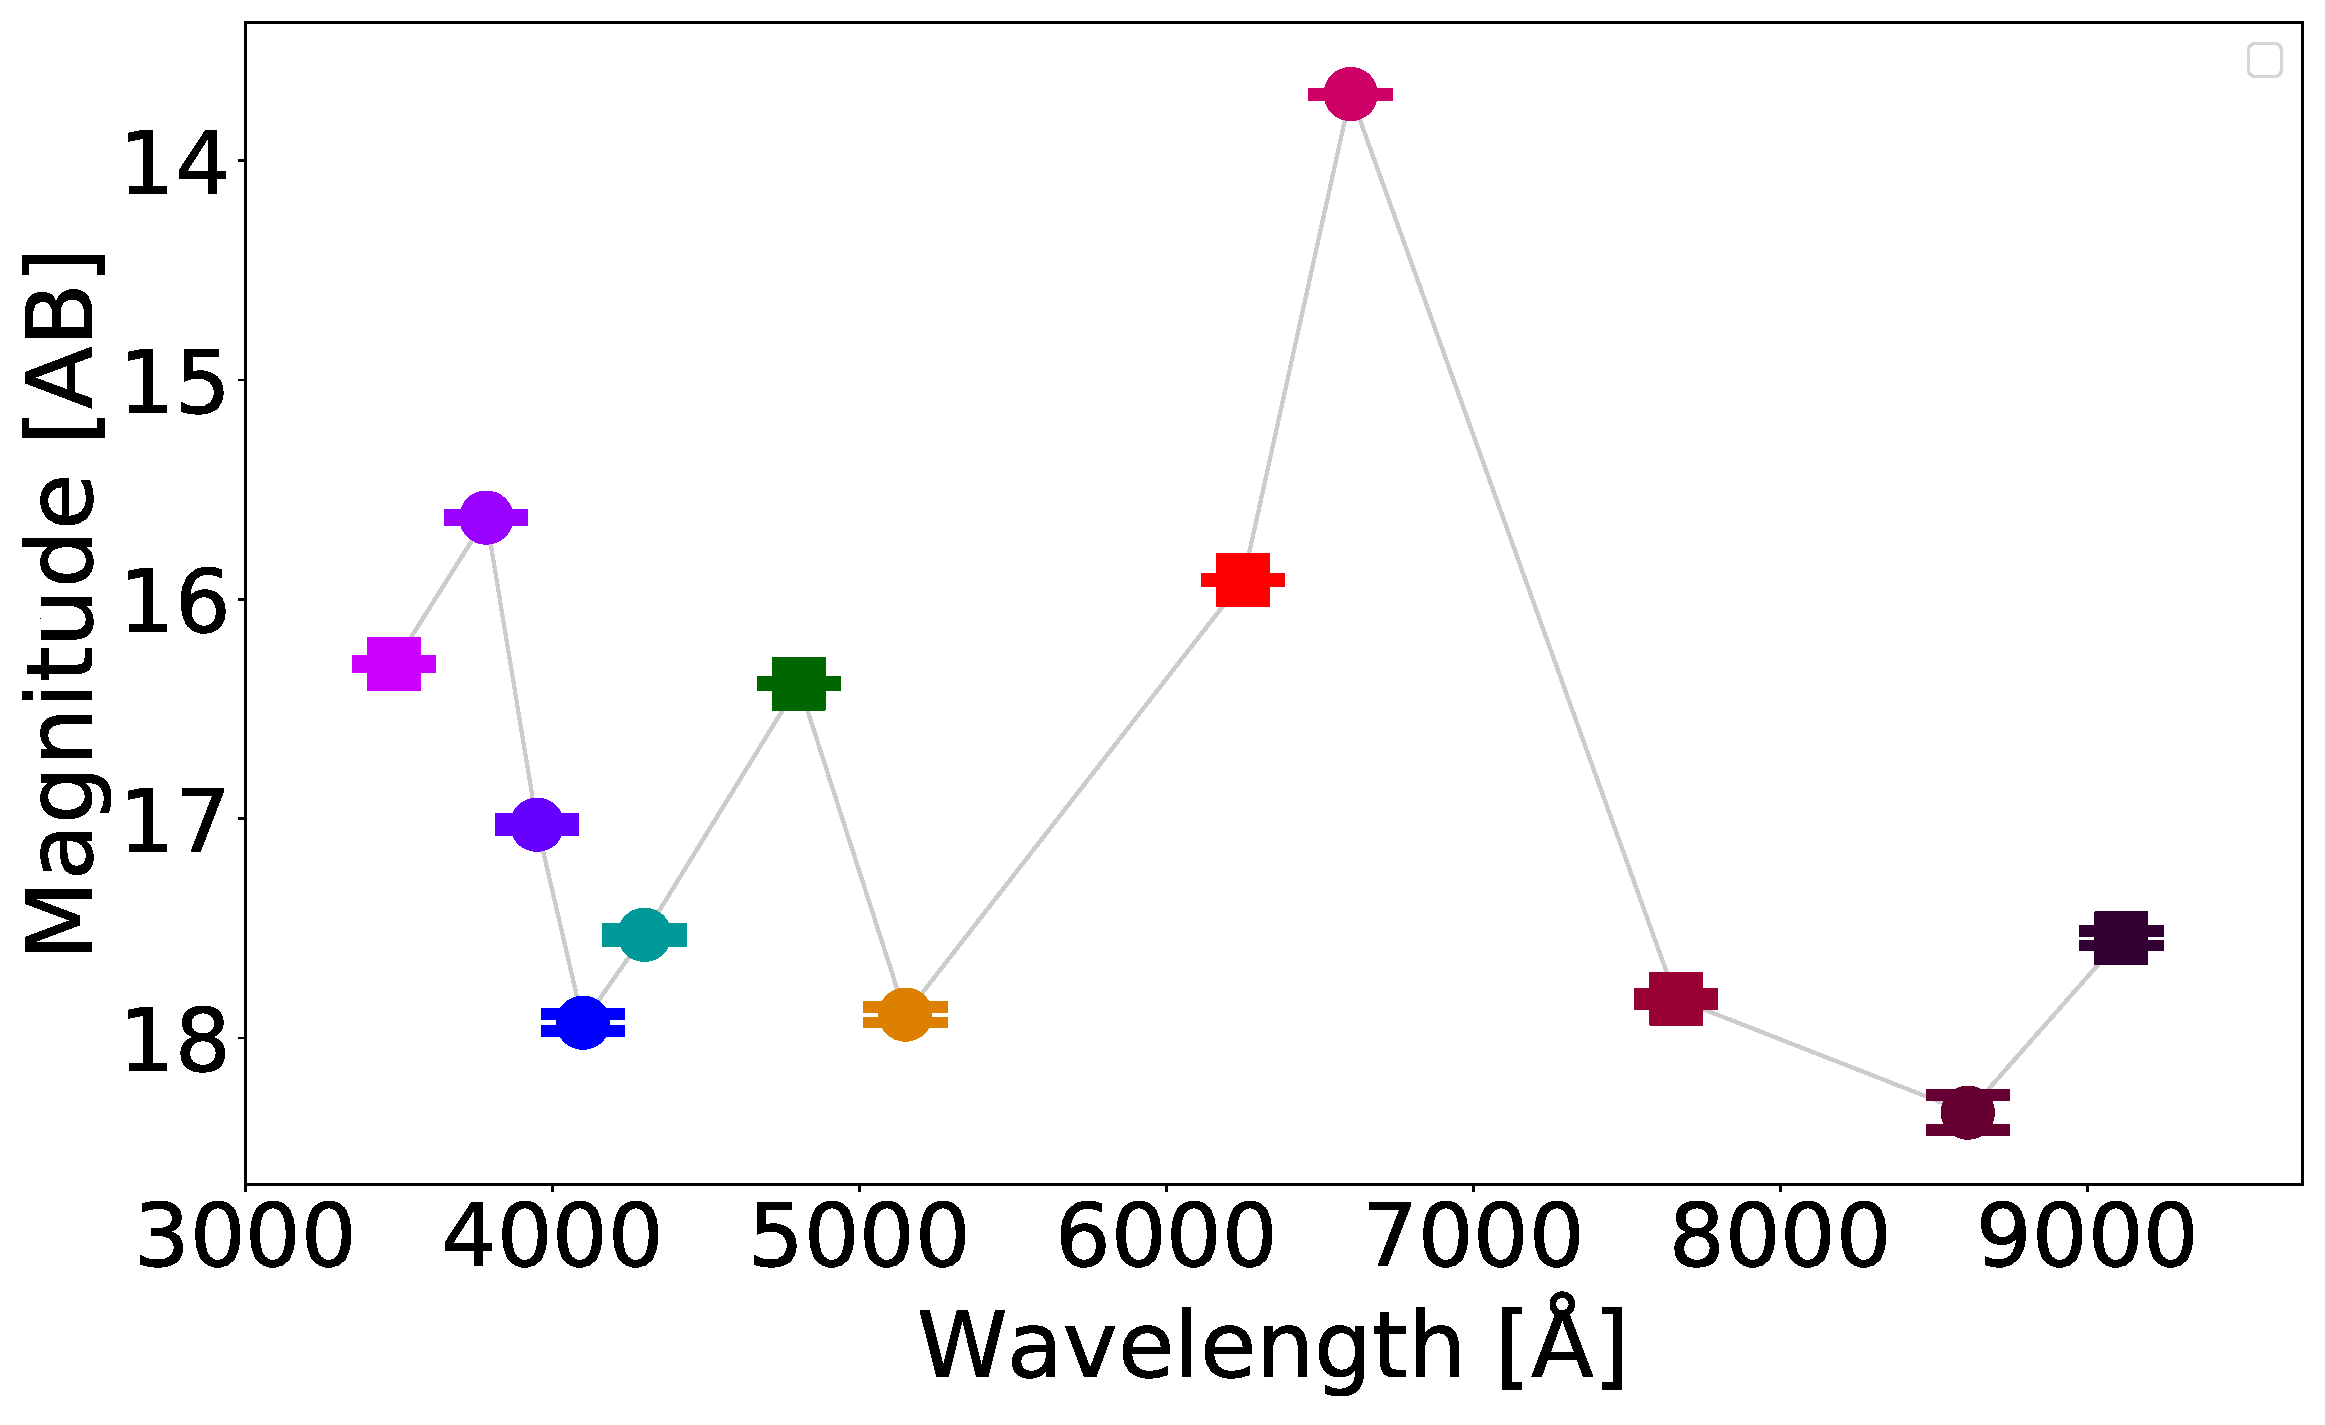
\includegraphics[width=0.3\linewidth, clip]{figs-pca/photospectrum_64078-73697-PN-pc-Halpha_emitters_threeerror-cleaning-limfilter-limcolor-flags-mask-broad_MAG_APER_6_0.pdf} & 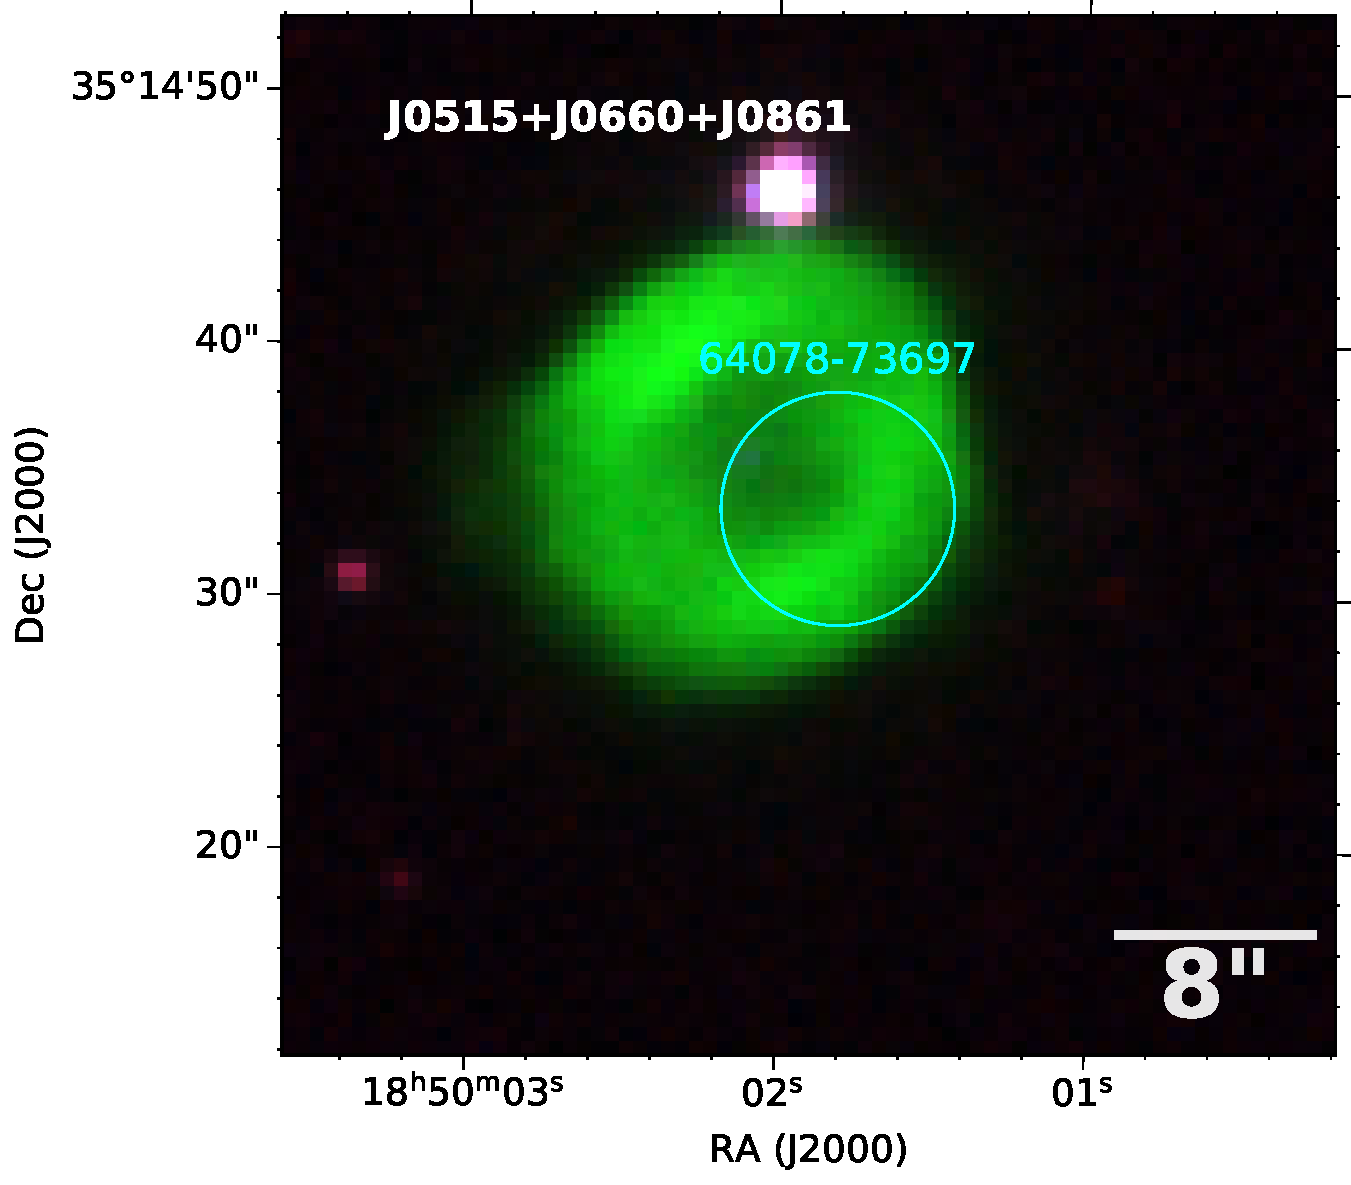
\includegraphics[width=0.3\linewidth, clip]{Field_64078/1000001-JPLUS-01172-v202006_J0861_64078-73697-RGB.pdf} & 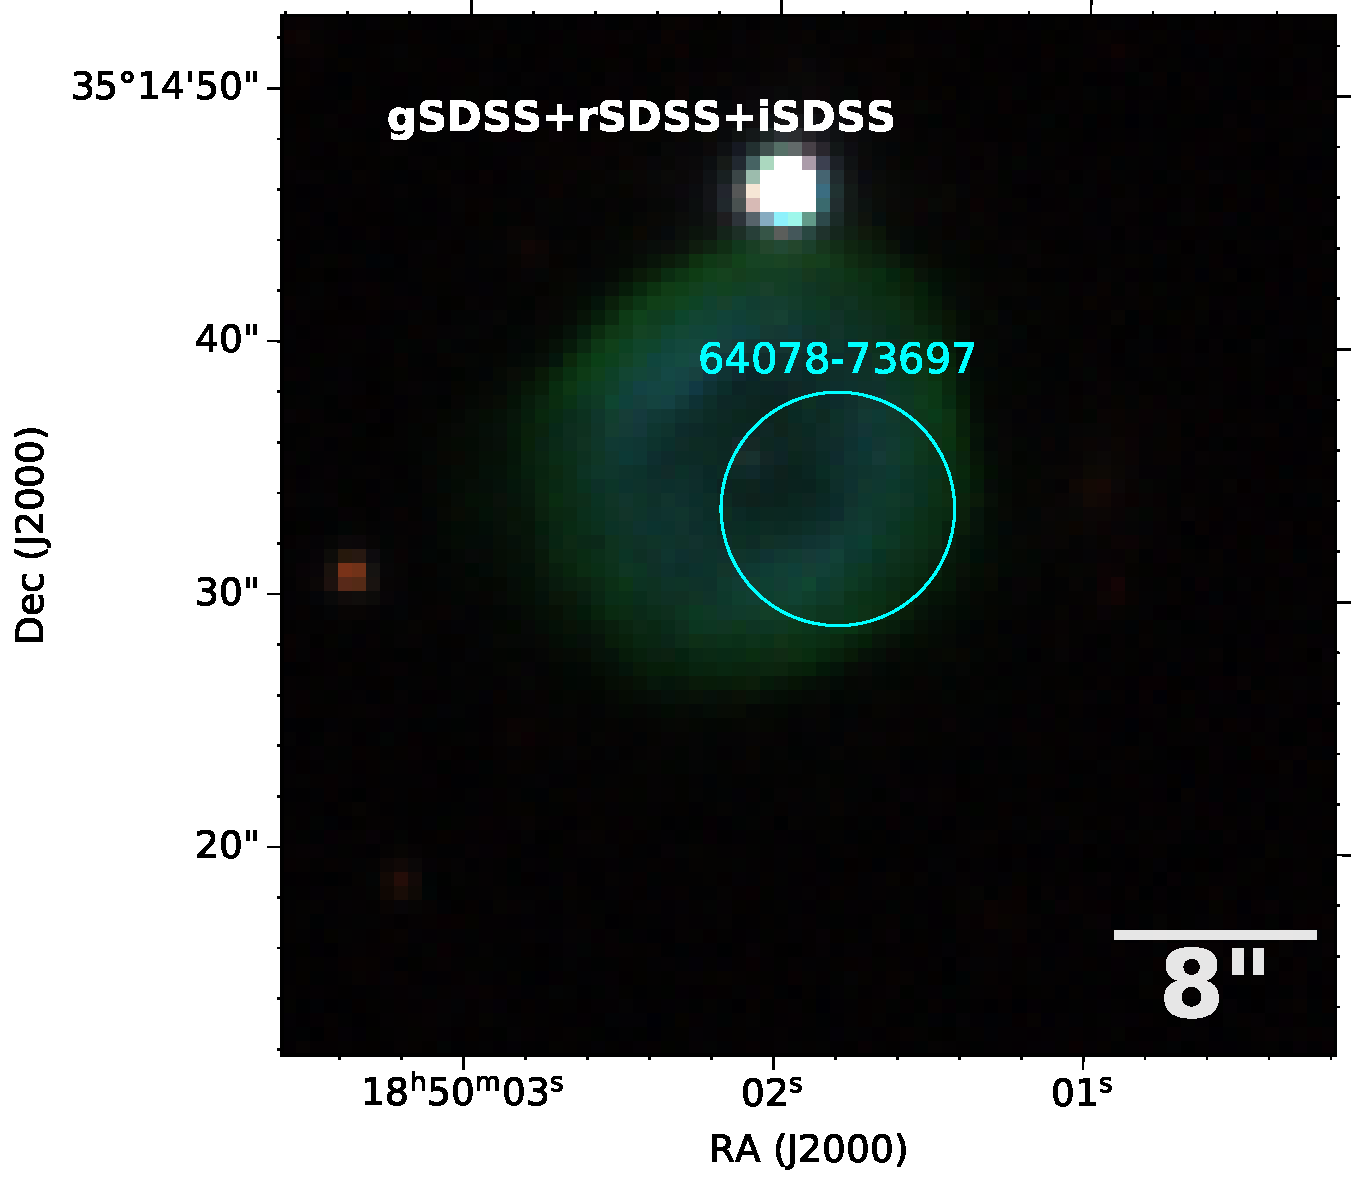
\includegraphics[width=0.3\linewidth, clip]{Field_64078/1000001-JPLUS-01172-v202006_iSDSS_64078-73697-RGB.pdf} \\
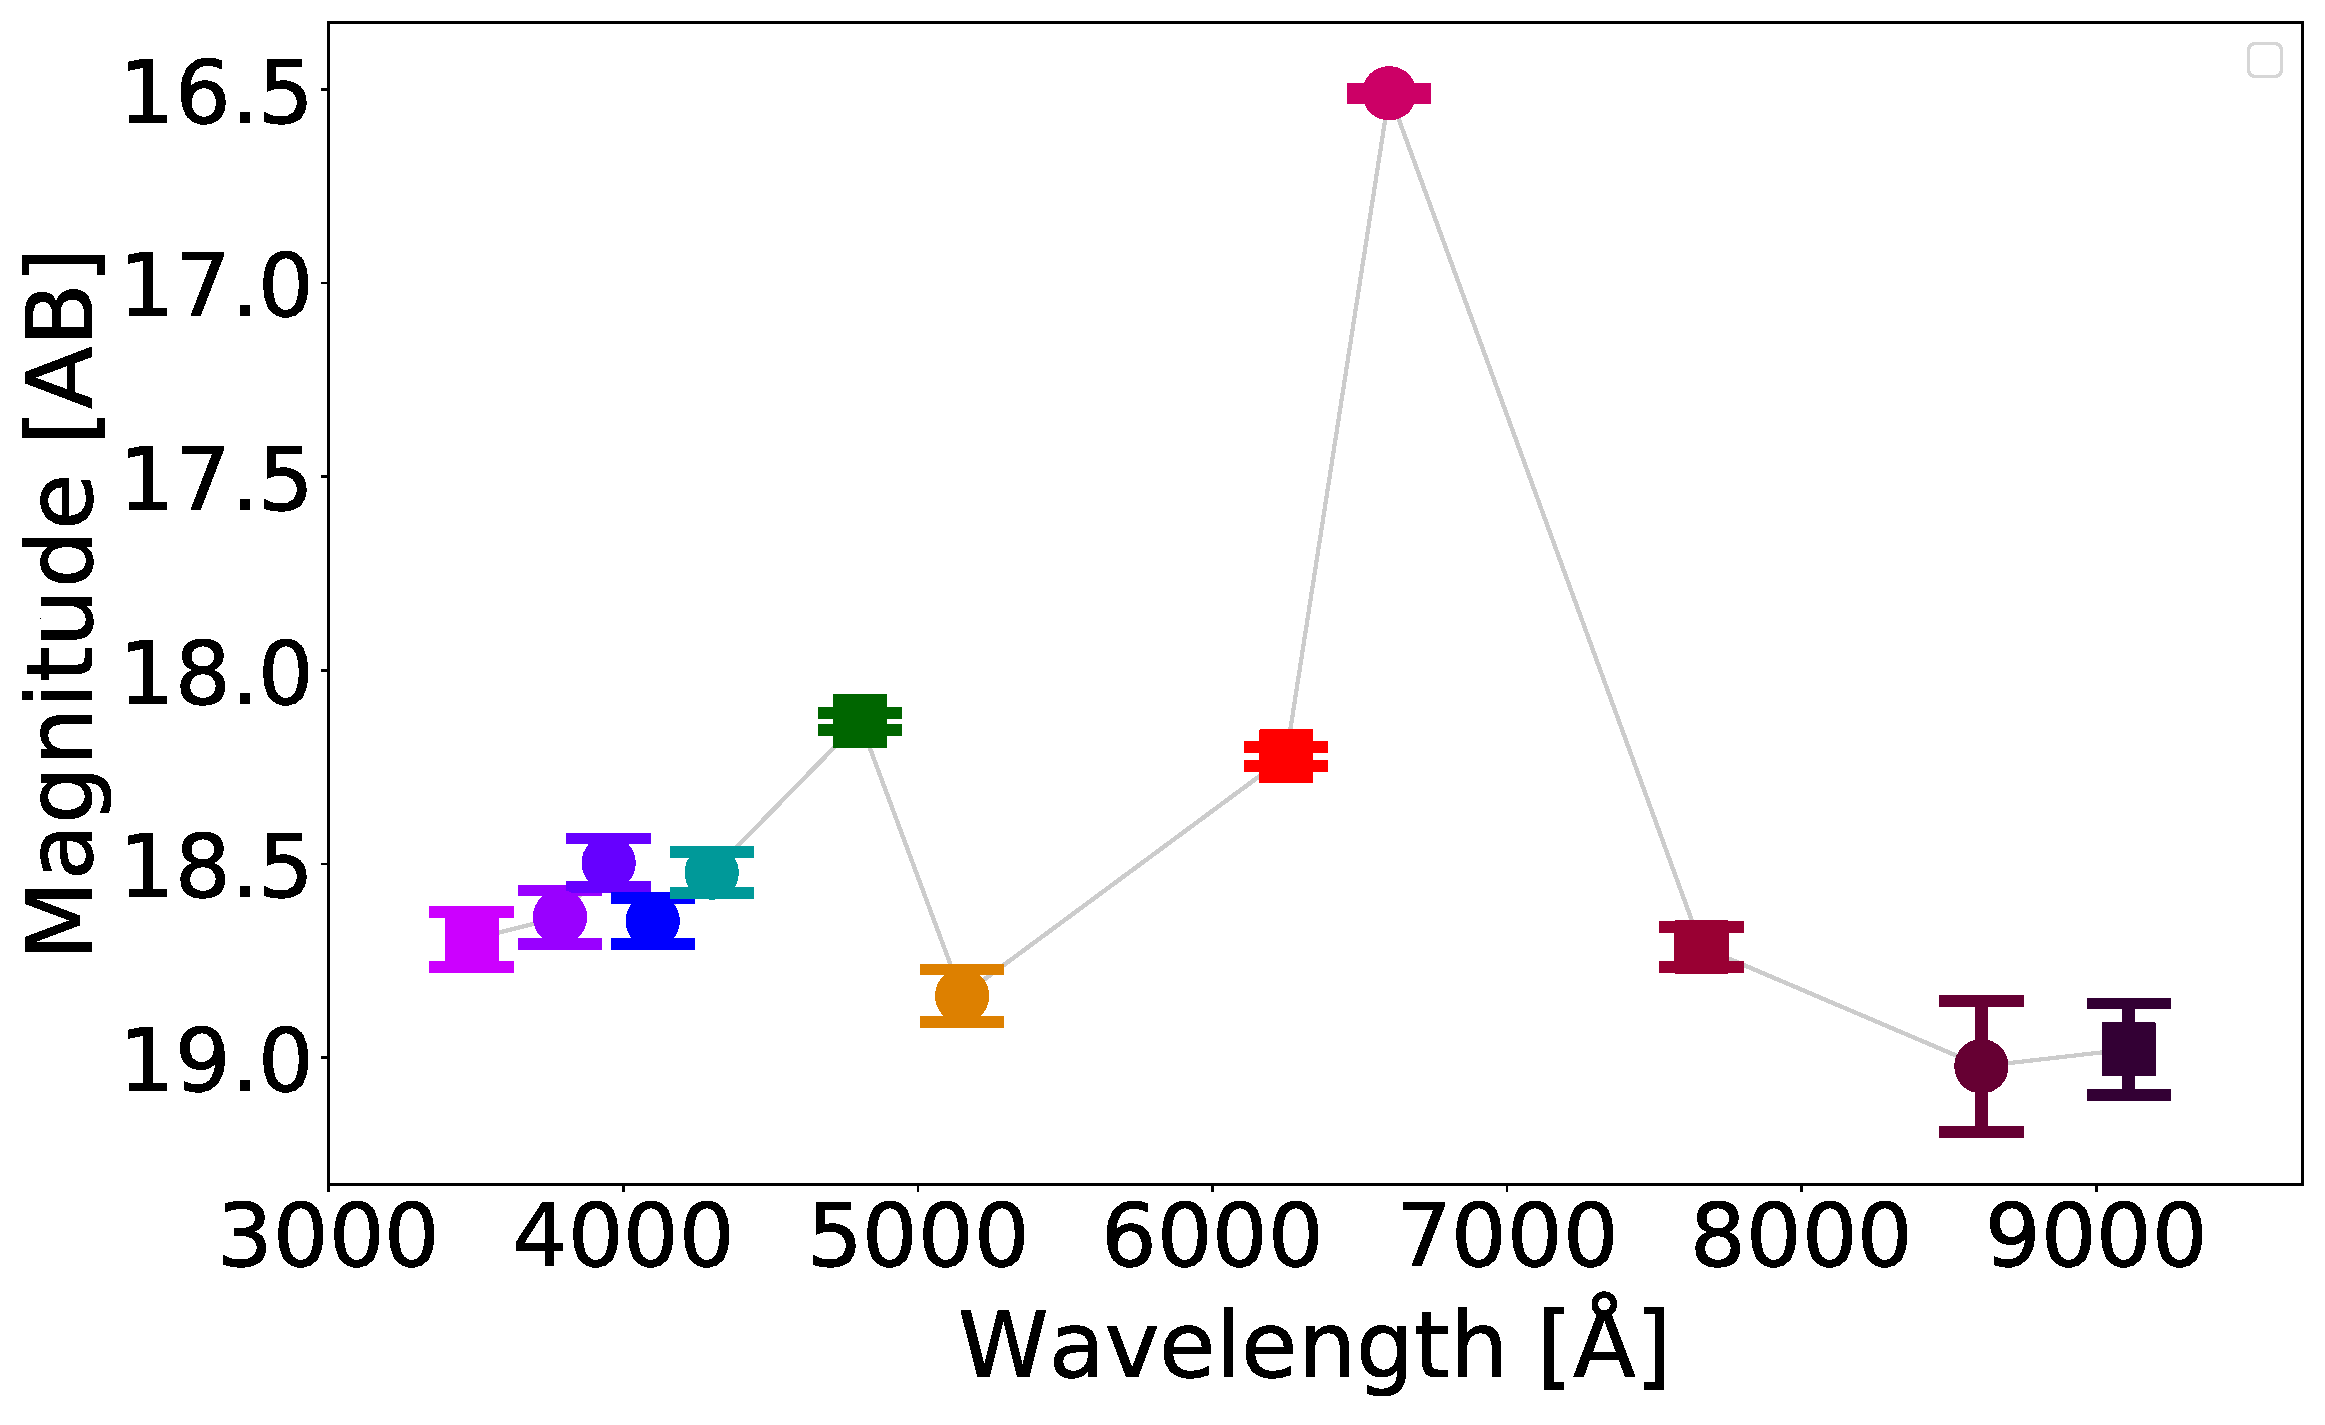
\includegraphics[width=0.3\linewidth, clip]{figs-pca/photospectrum_64138-3942-PN-pc-Halpha_emitters_threeerror-cleaning-limfilter-limcolor-flags-mask-broad_MAG_APER_6_0.pdf} & 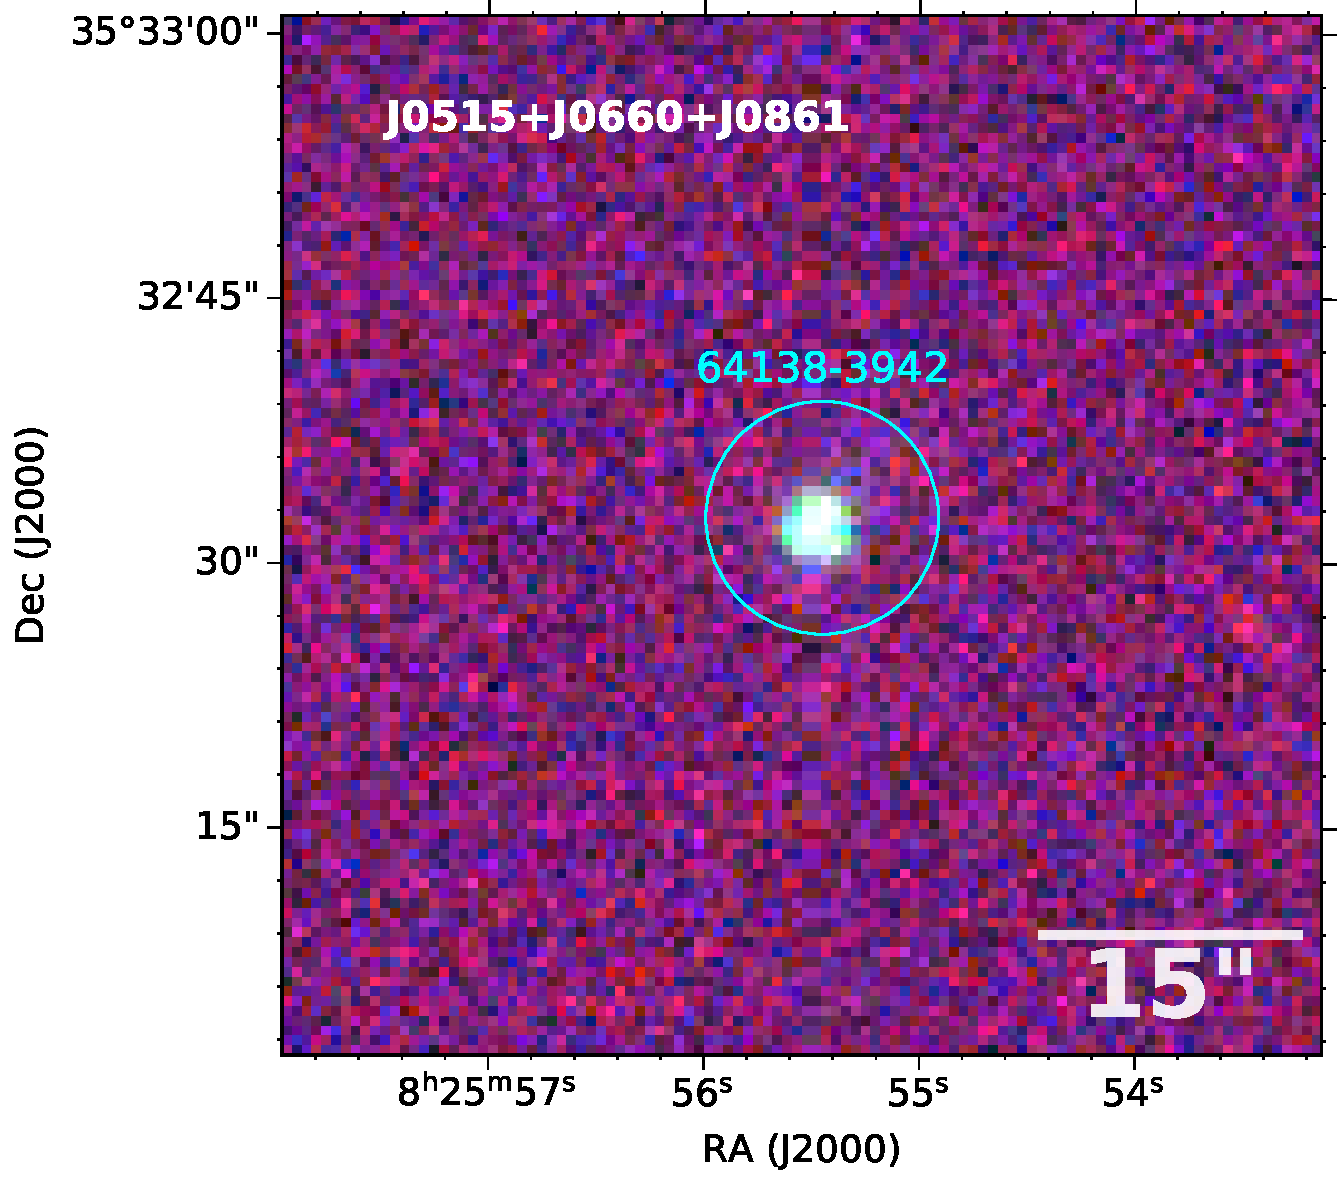
\includegraphics[width=0.3\linewidth, clip]{Field_64138/1000001-JPLUS-01186-v202006_J0861_64138-3942-RGB.pdf} & 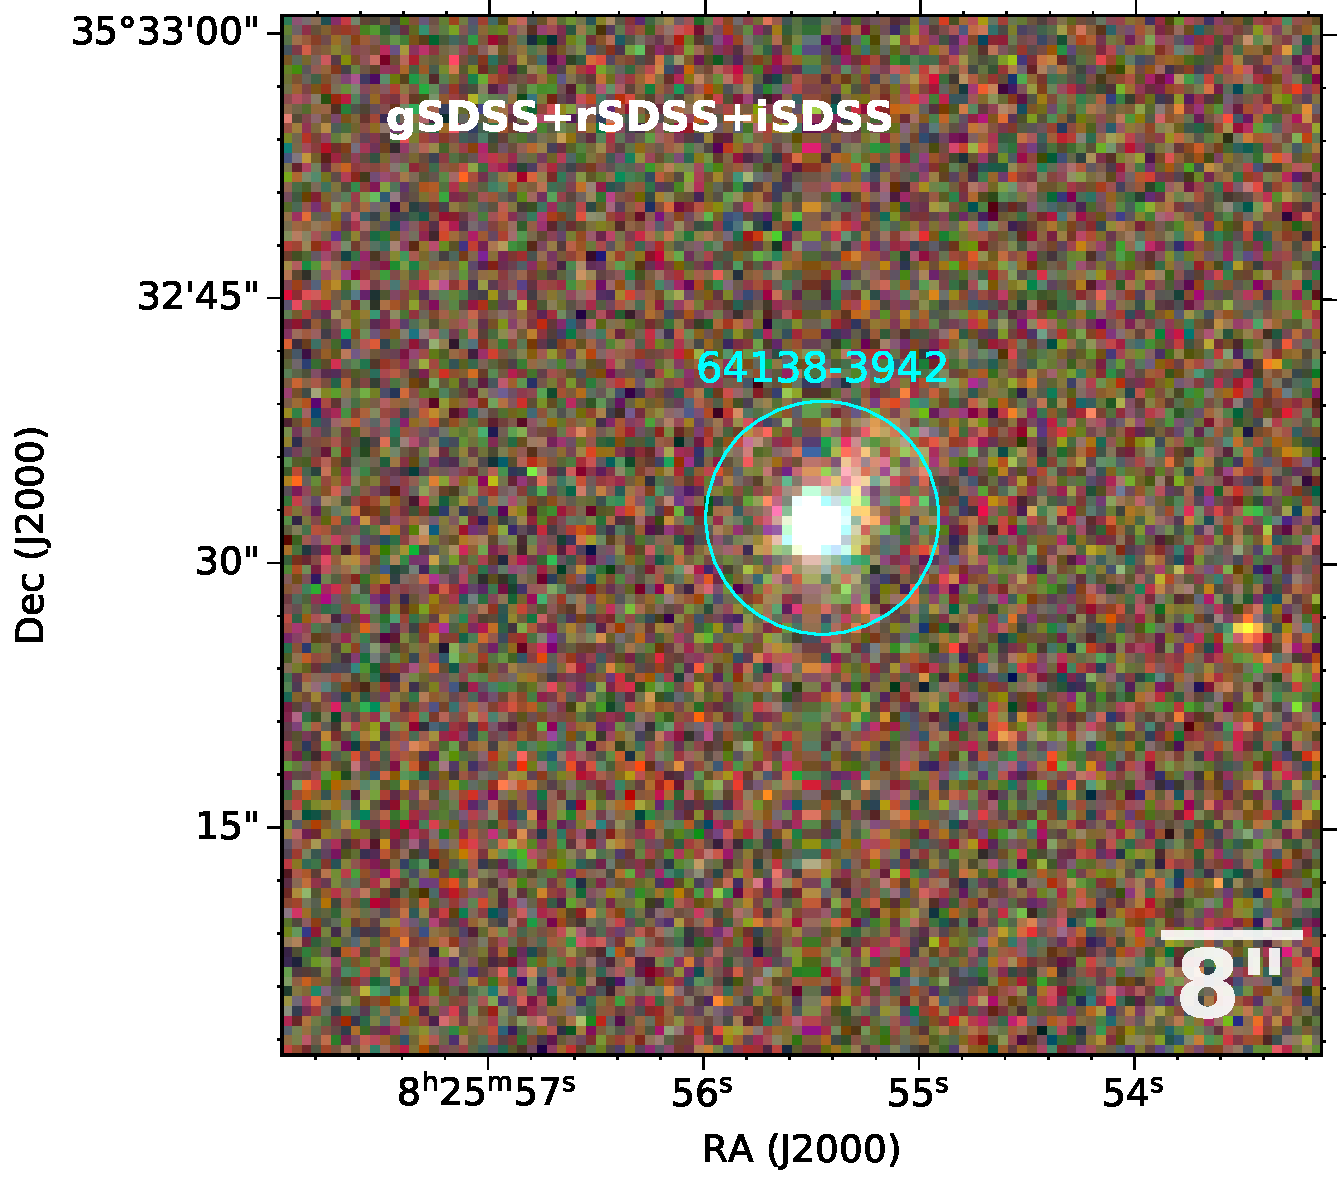
\includegraphics[width=0.3\linewidth, clip]{Field_64138/1000001-JPLUS-01186-v202006_iSDSS_64138-3942-RGB.pdf} \\
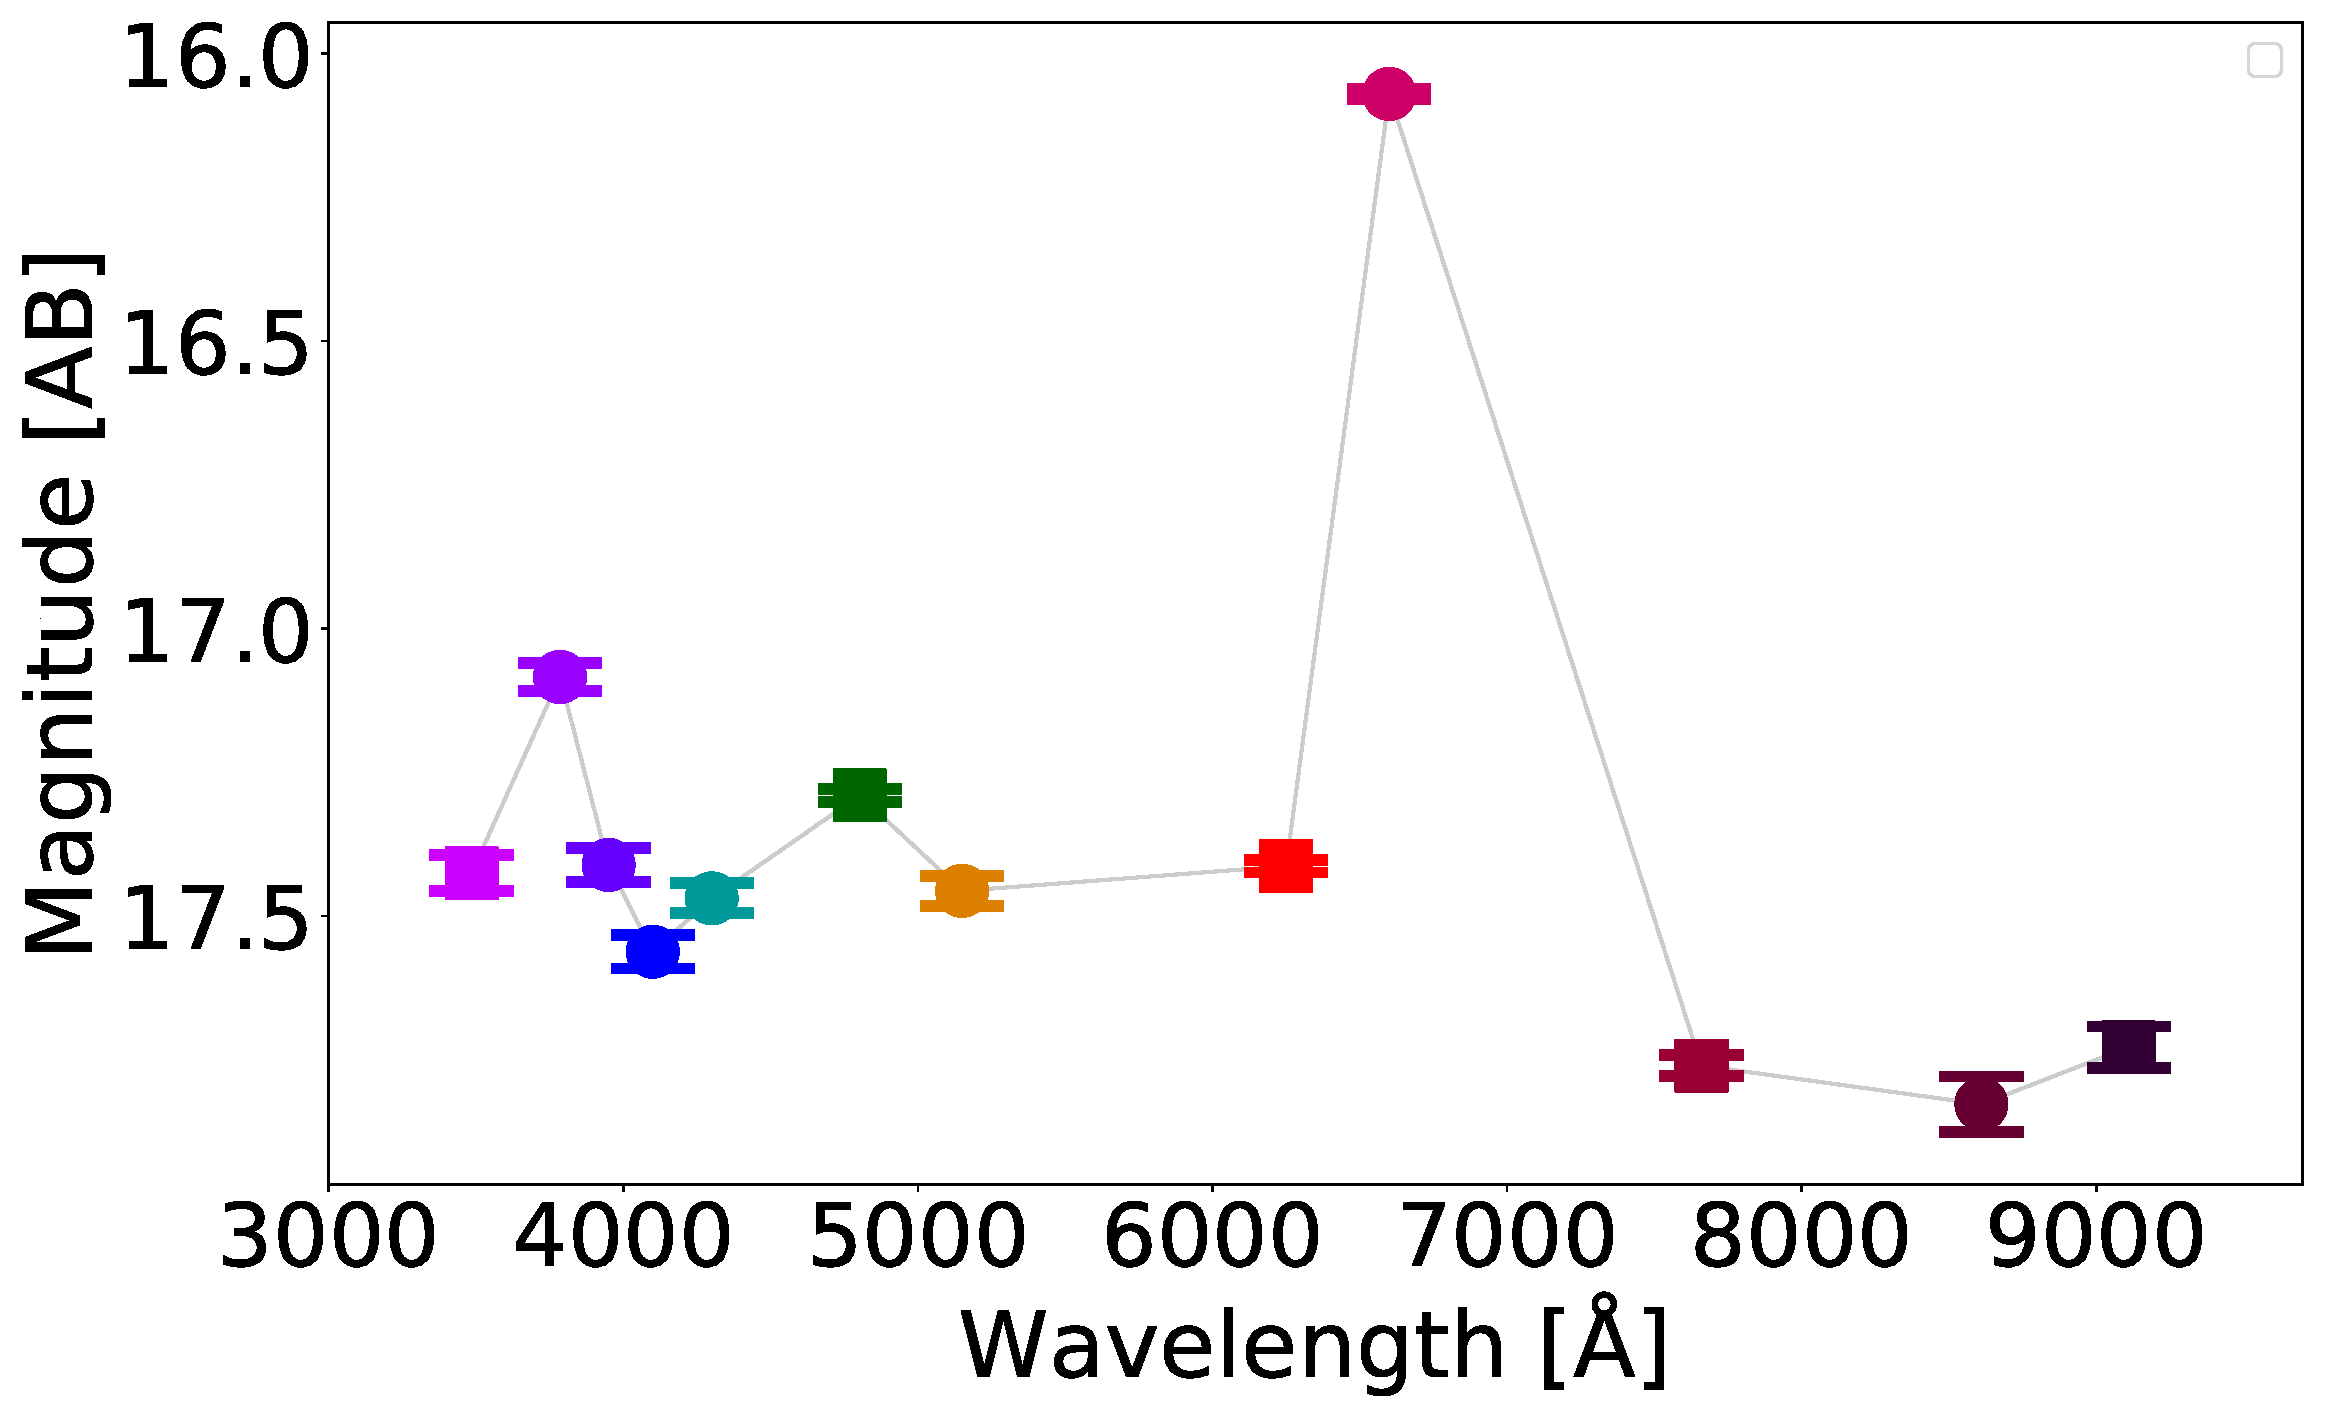
\includegraphics[width=0.3\linewidth, clip]{figs-pca/photospectrum_64235-10908-PN-pc-Halpha_emitters_threeerror-cleaning-limfilter-limcolor-flags-mask-broad_MAG_APER_6_0.pdf} & 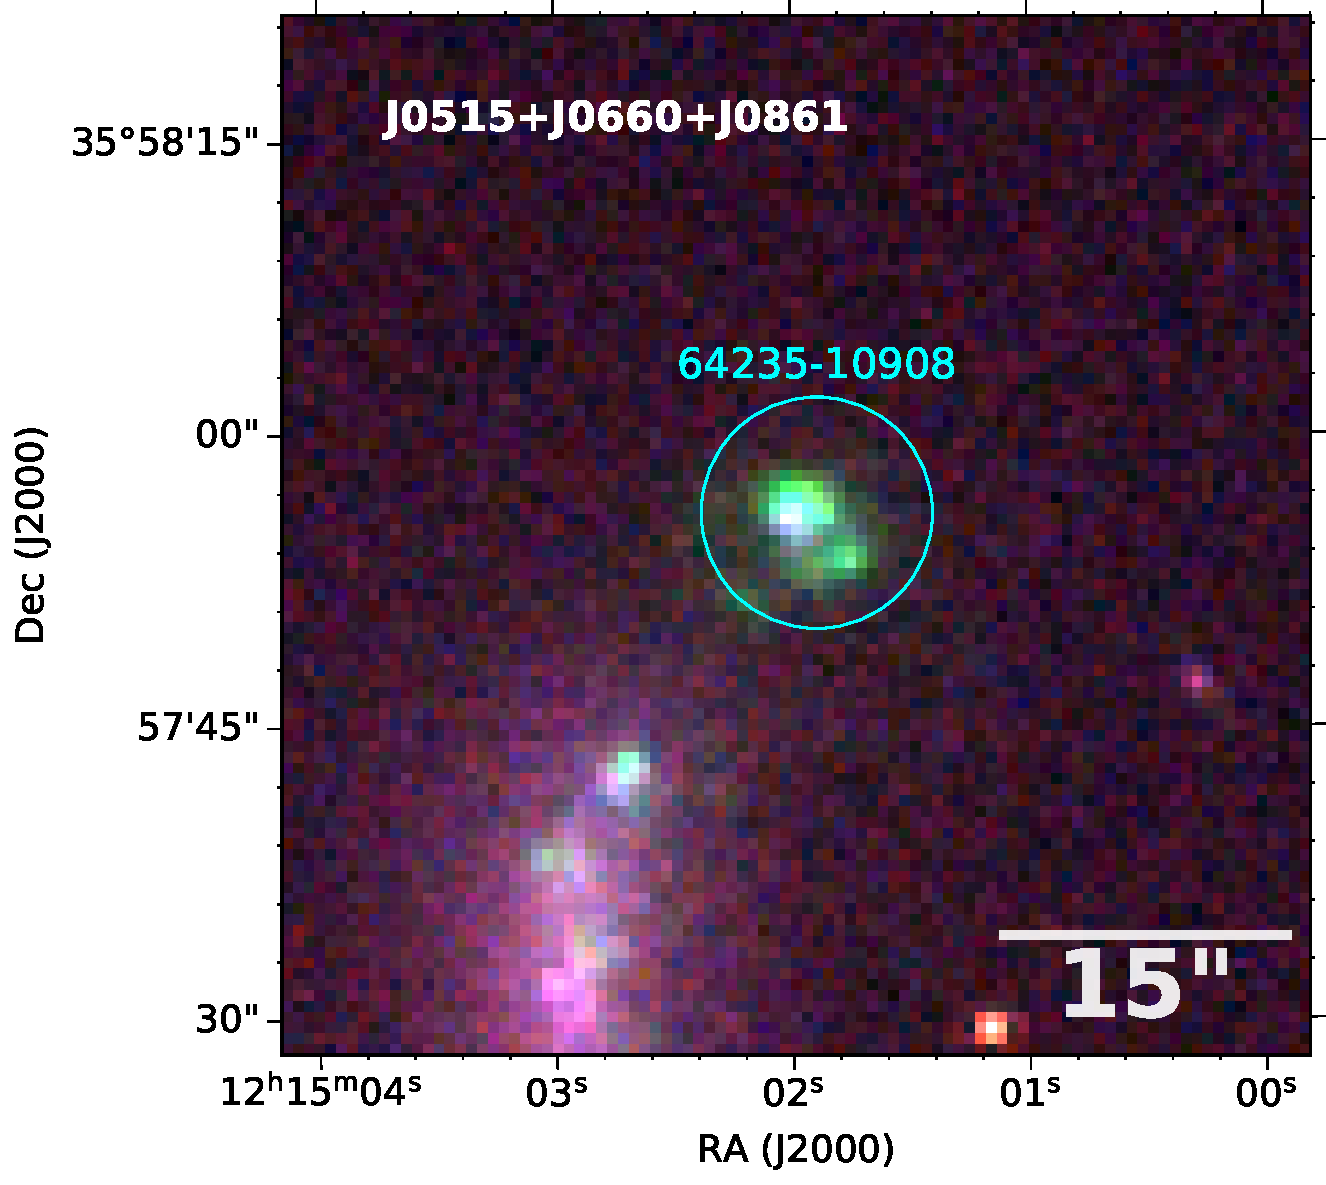
\includegraphics[width=0.3\linewidth, clip]{Field_64235/1000001-JPLUS-01220-v202006_J0861_64235-10908-RGB.pdf} & 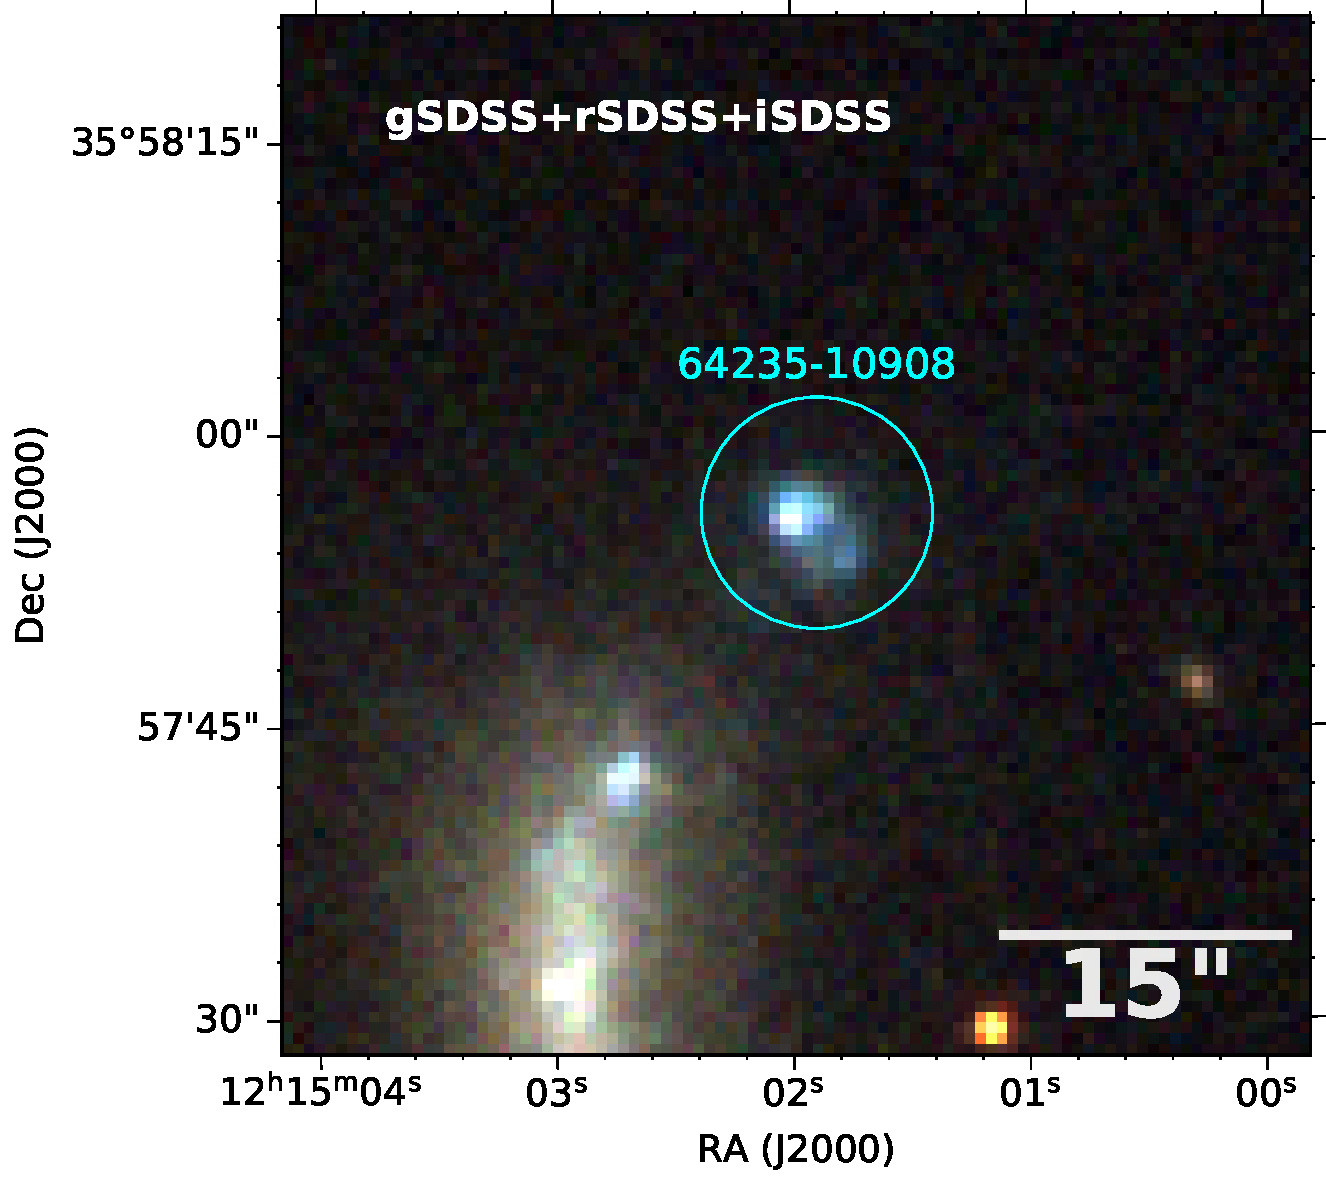
\includegraphics[width=0.3\linewidth, clip]{Field_64235/1000001-JPLUS-01220-v202006_iSDSS_64235-10908-RGB.pdf} \\
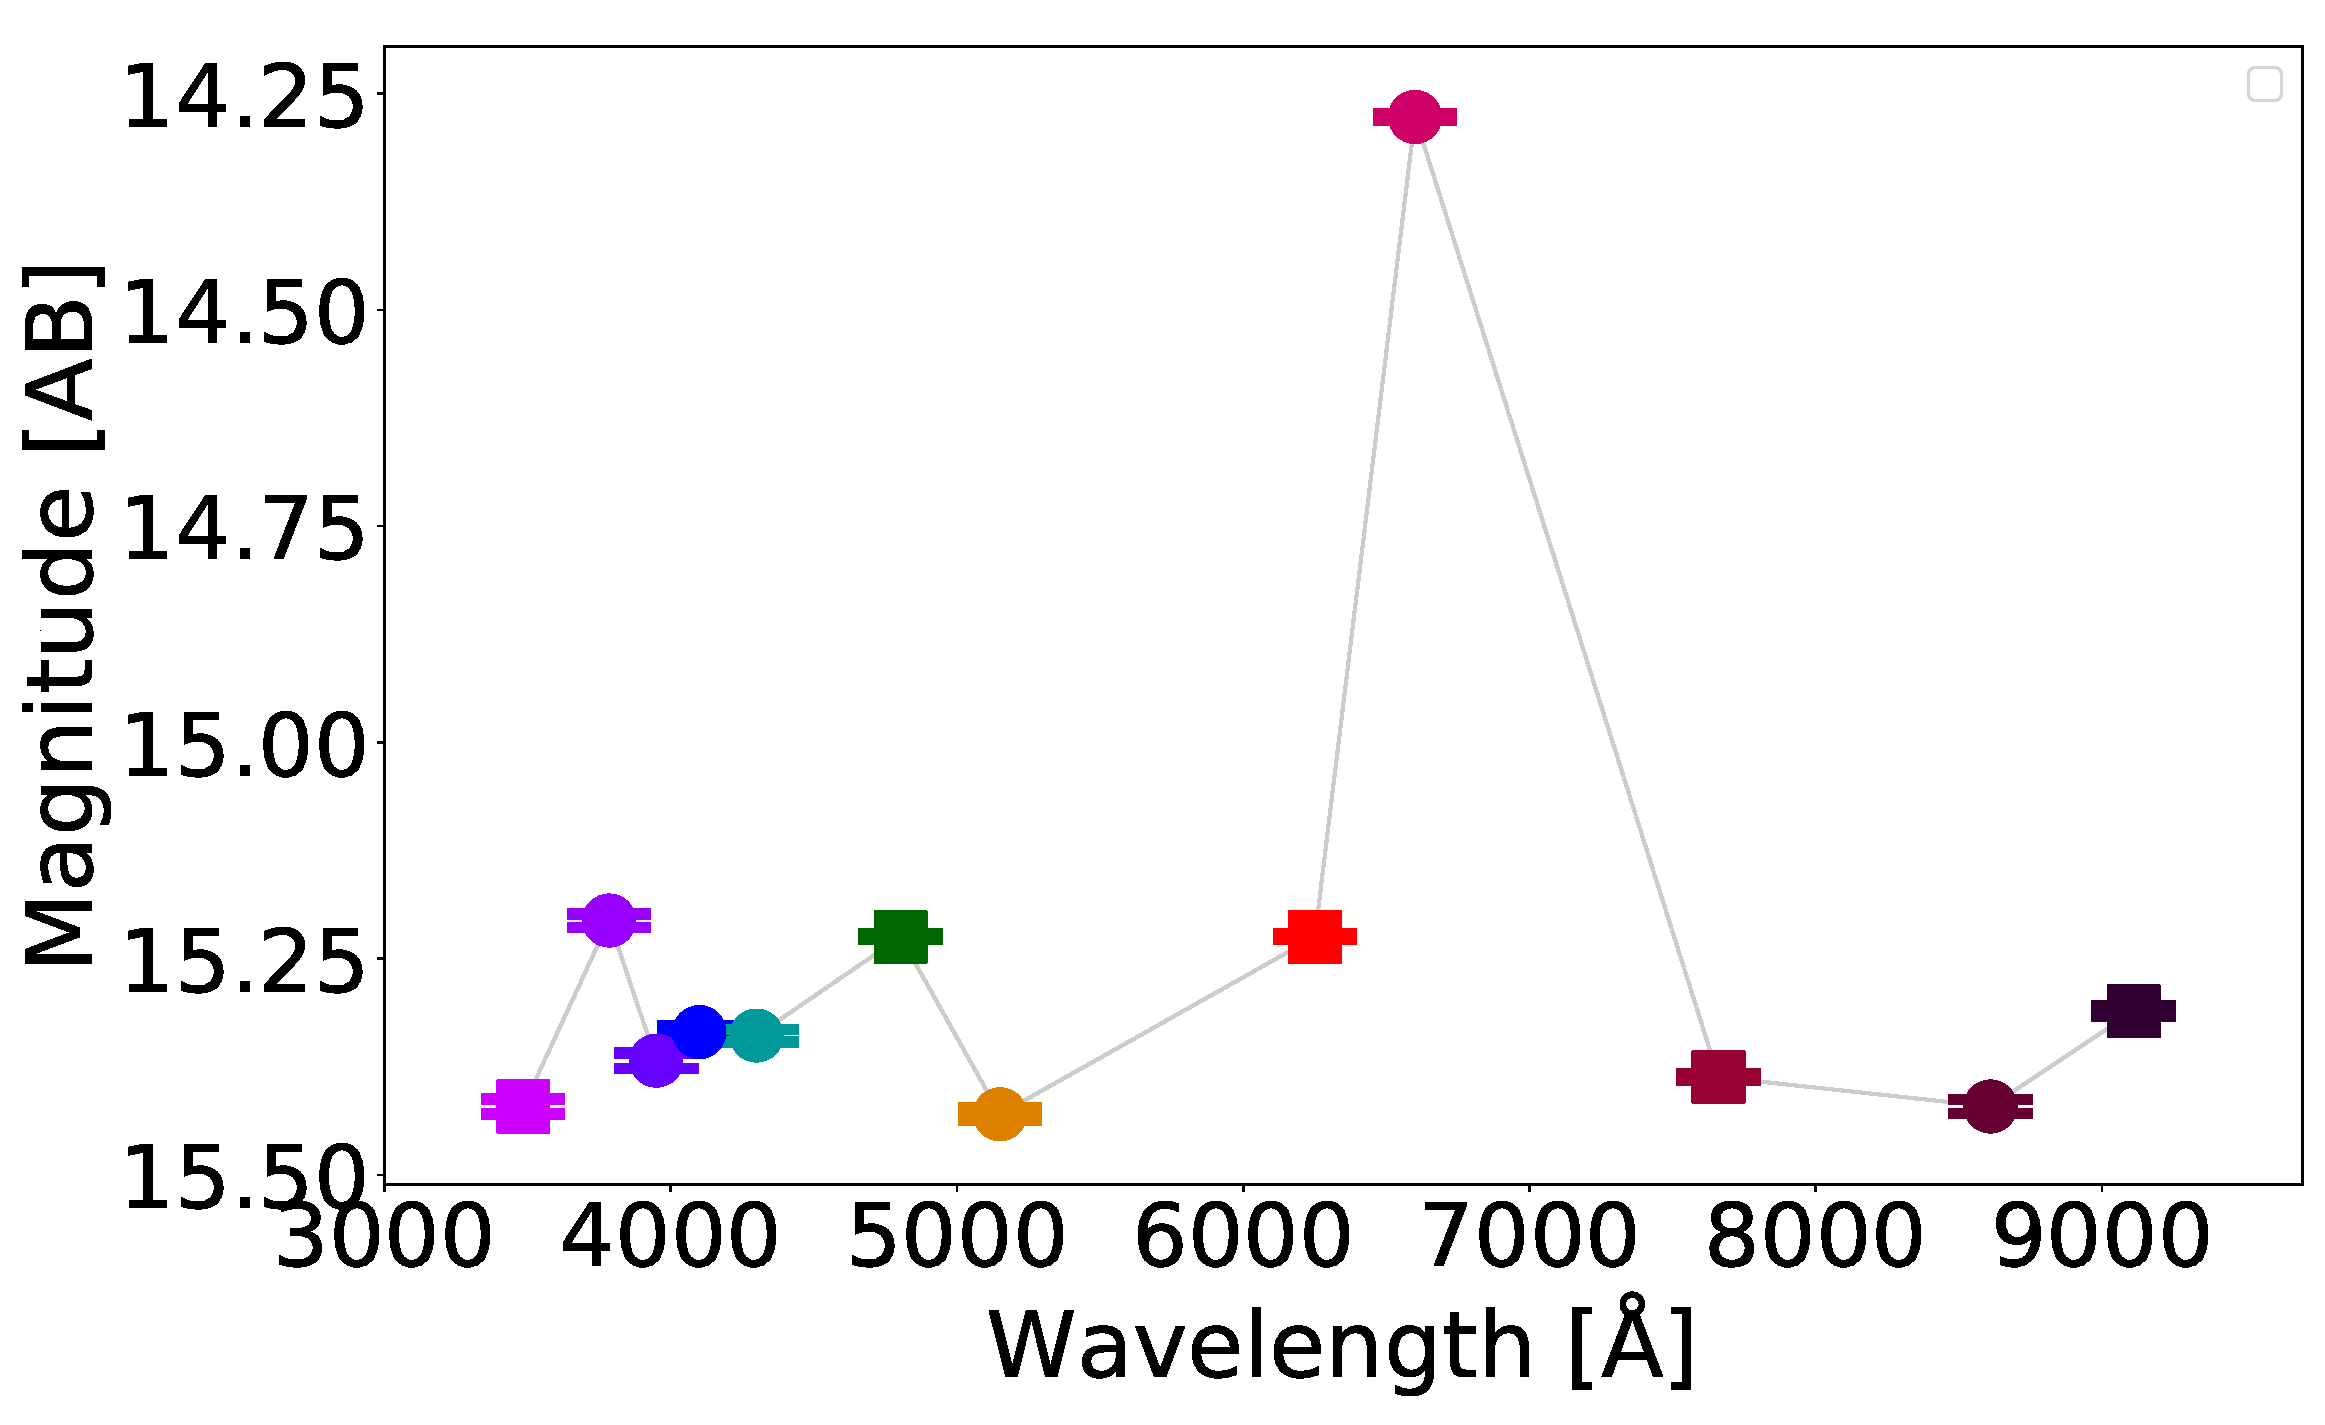
\includegraphics[width=0.3\linewidth, clip]{figs-pca/photospectrum_64235-12290-PN-pc-Halpha_emitters_threeerror-cleaning-limfilter-limcolor-flags-mask-broad_MAG_APER_6_0.pdf} & 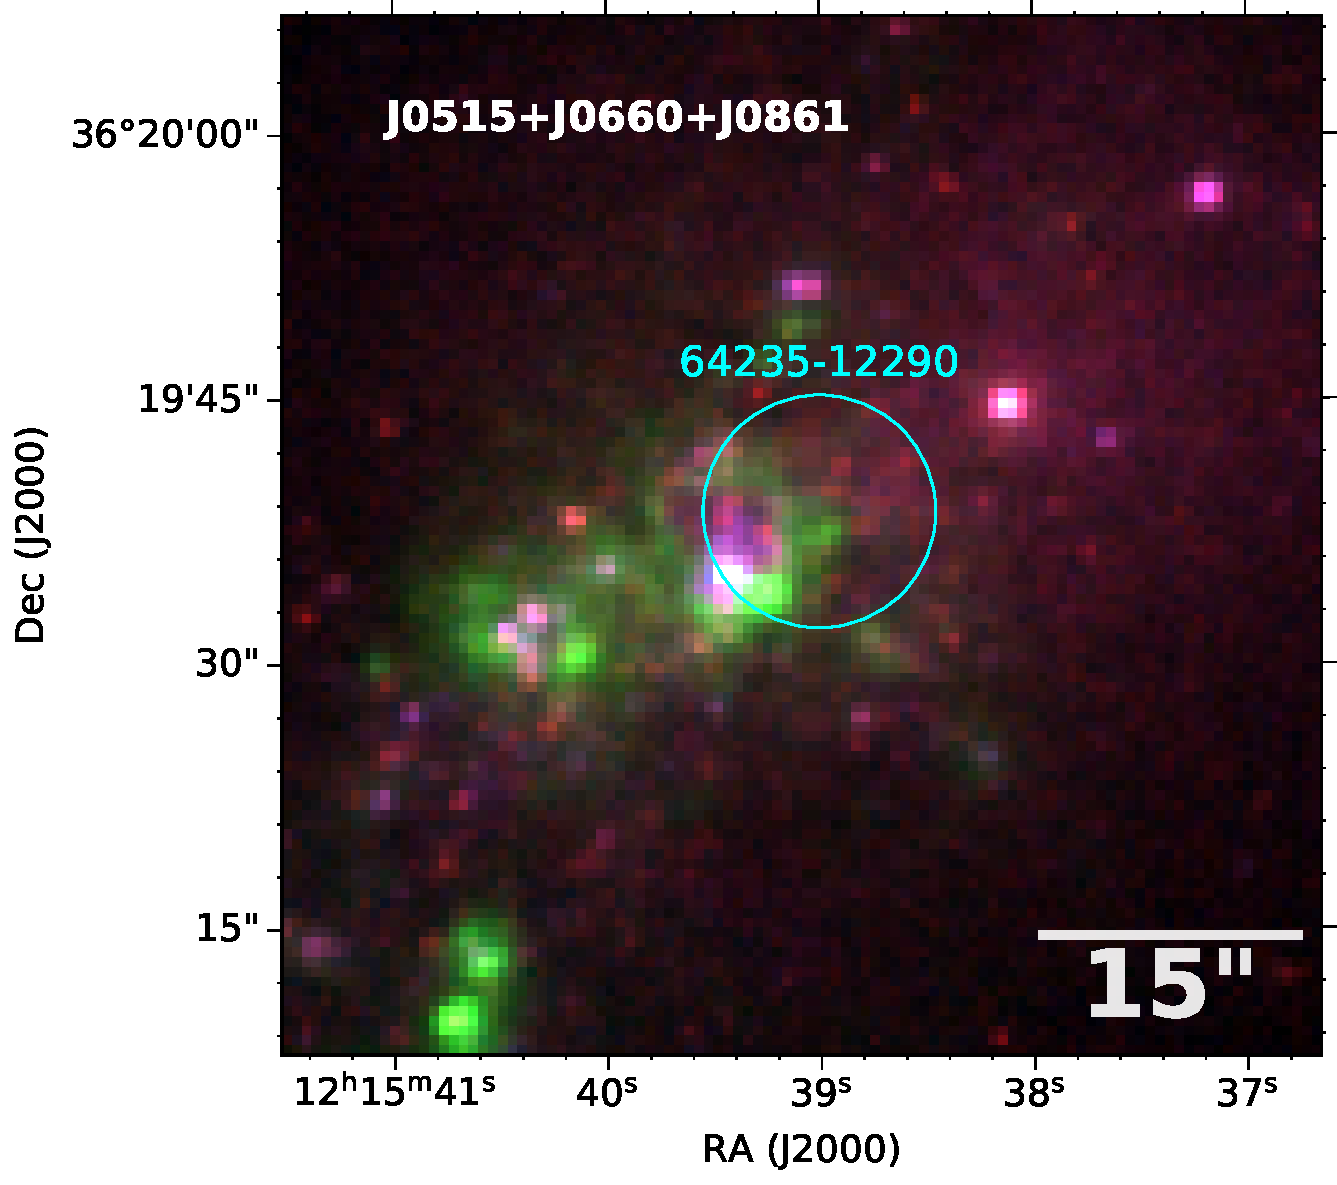
\includegraphics[width=0.3\linewidth, clip]{Field_64235/1000001-JPLUS-01220-v202006_J0861_64235-12290-RGB.pdf} & 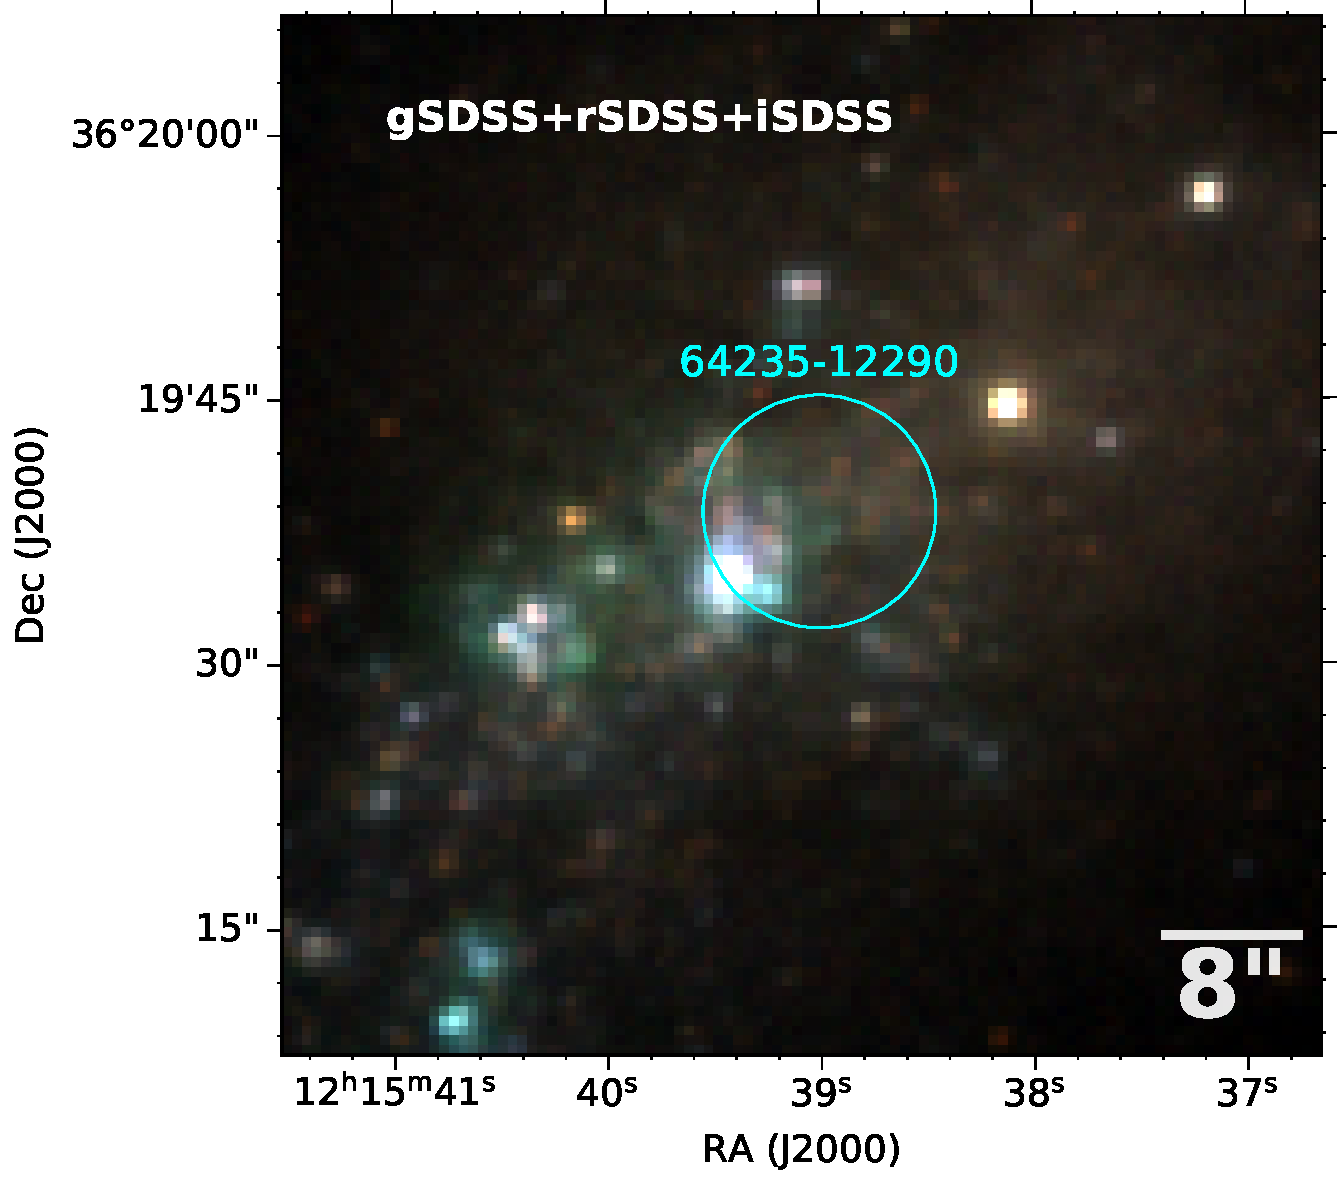
\includegraphics[width=0.3\linewidth, clip]{Field_64235/1000001-JPLUS-01220-v202006_iSDSS_64235-12290-RGB.pdf} \\
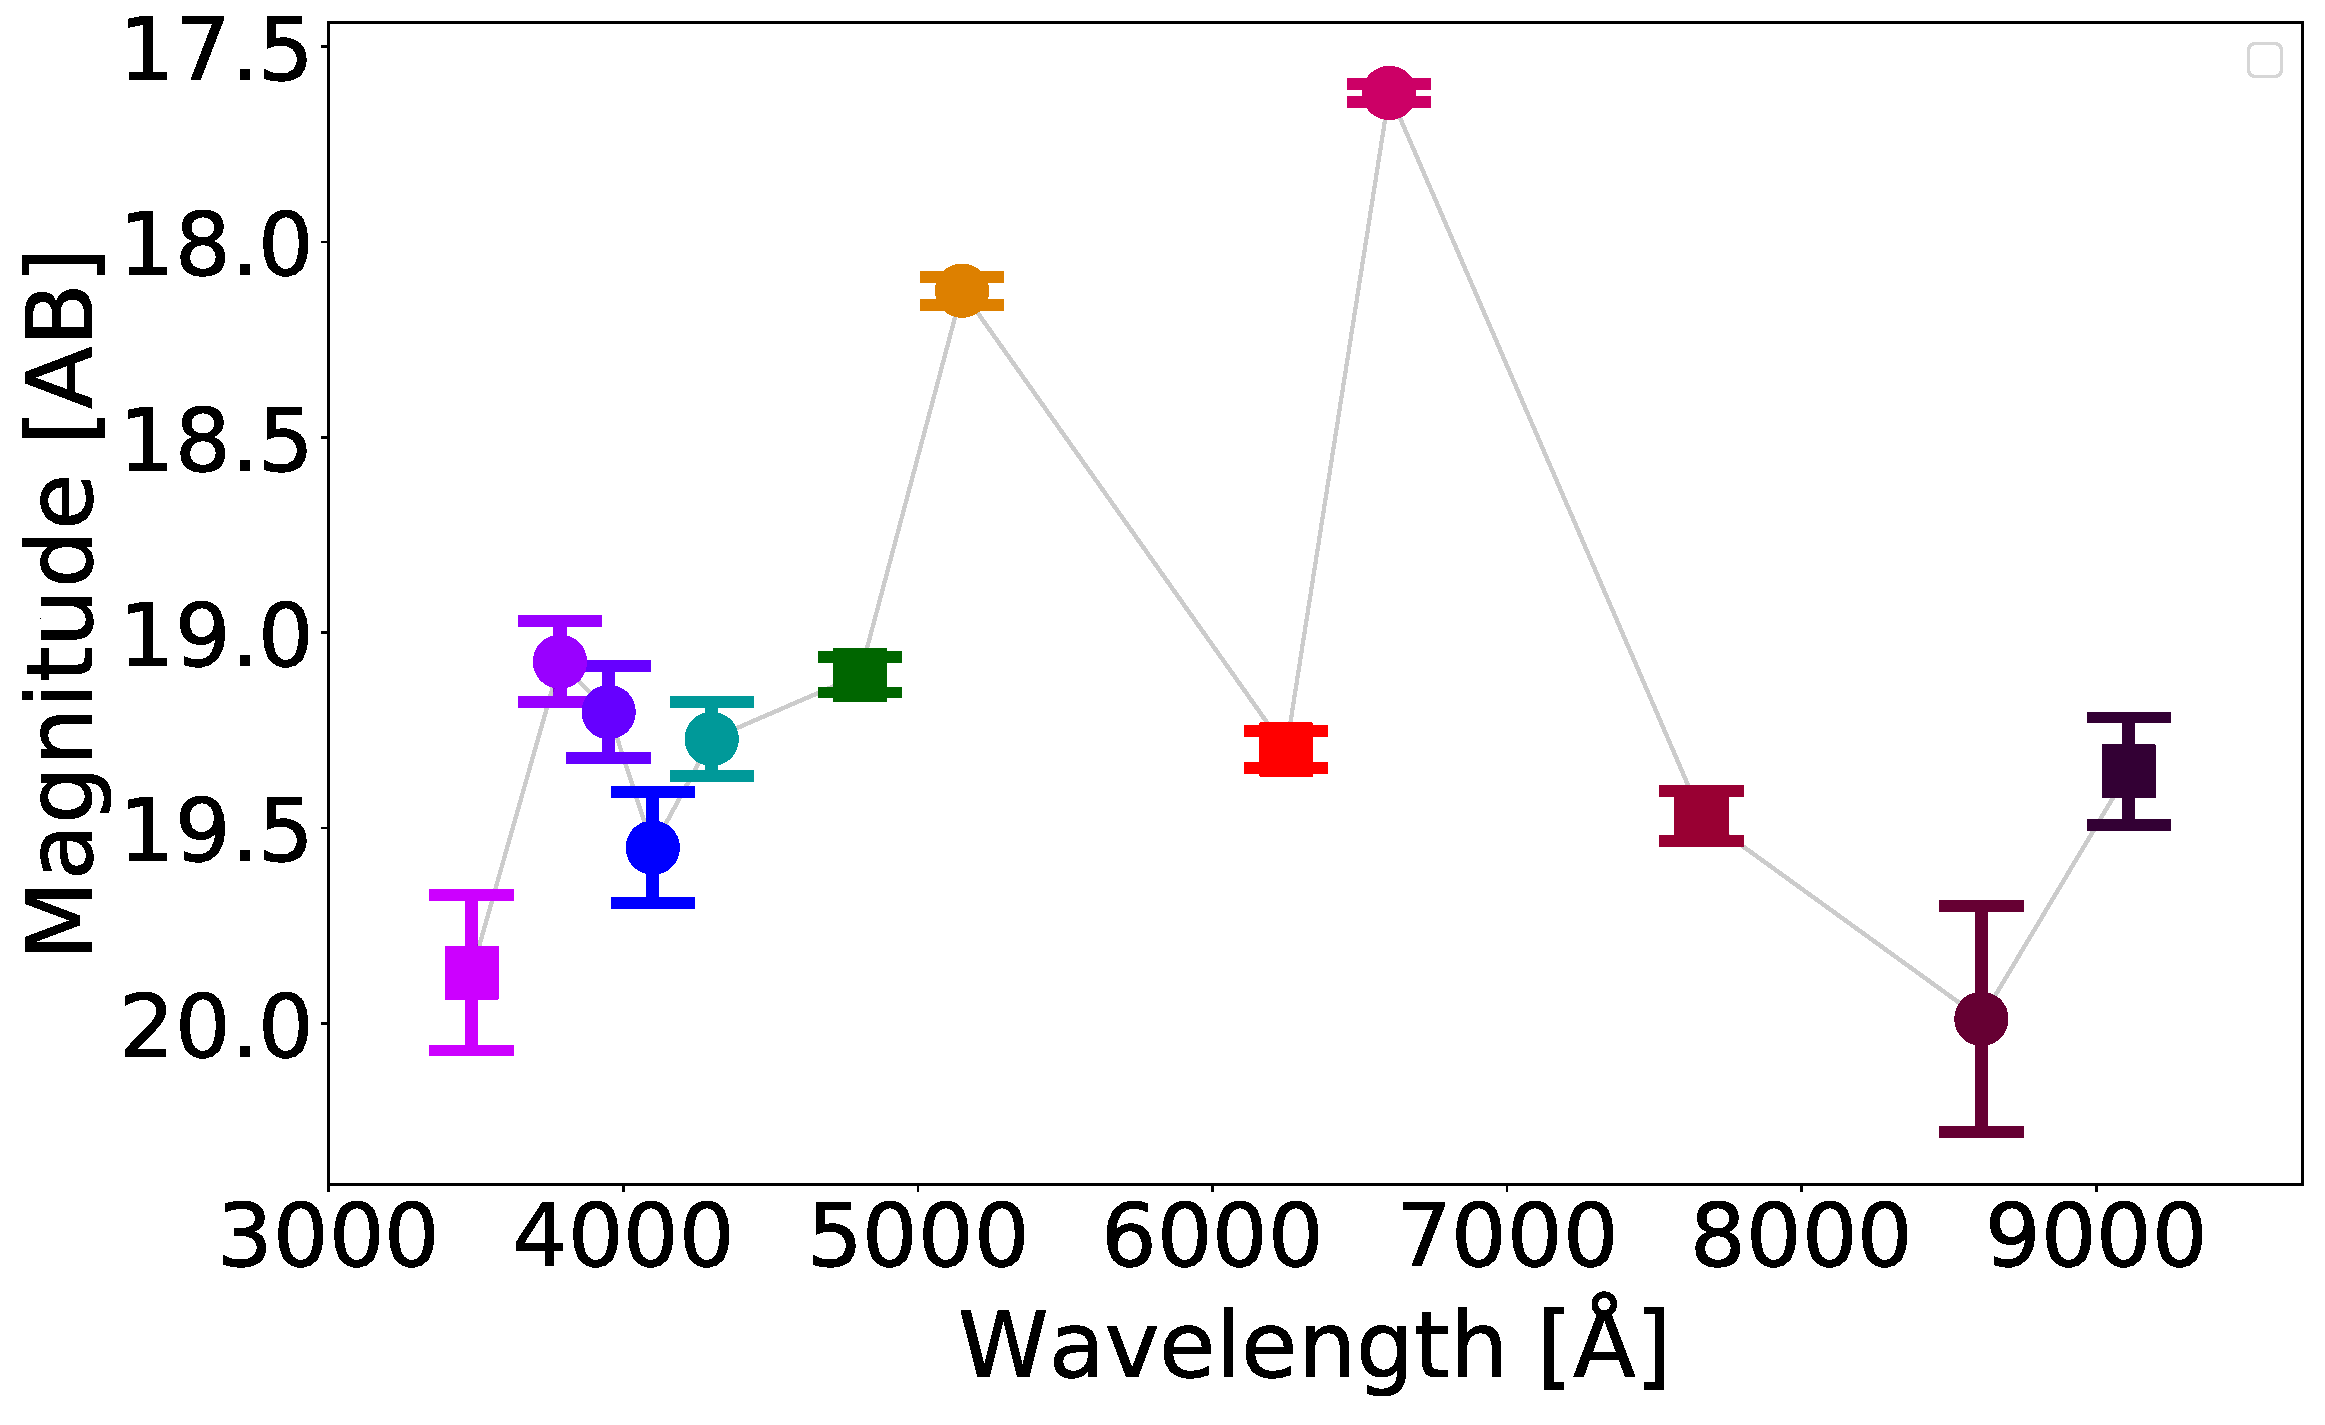
\includegraphics[width=0.3\linewidth, clip]{figs-pca/photospectrum_64626-37444-PN-pc-Halpha_emitters_threeerror-cleaning-limfilter-limcolor-flags-mask-broad_MAG_APER_6_0.pdf} & \includegraphics[width=0.3\linewidth, clip]{Field_64626/1000001-JPLUS-01374-v202006_J0861_64626-37444-RGB.pdf} & \includegraphics[width=0.3\linewidth, clip]{Field_64626/1000001-JPLUS-01374-v202006_iSDSS_64626-37444-RGB.pdf} \\
\includegraphics[width=0.3\linewidth, clip]{figs-pca/photospectrum_65478-6149-PN-pc-Halpha_emitters_threeerror-cleaning-limfilter-limcolor-flags-mask-broad_MAG_APER_6_0.pdf} & \includegraphics[width=0.3\linewidth, clip]{Field_65478/1000001-JPLUS-01504-v202006_J0861_65478-6149-RGB.pdf} & \includegraphics[width=0.3\linewidth, clip]{Field_65478/1000001-JPLUS-01504-v202006_iSDSS_65478-6149-RGB.pdf} \\
\includegraphics[width=0.3\linewidth, clip]{figs-pca/photospectrum_65478-6156-PN-pc-Halpha_emitters_threeerror-cleaning-limfilter-limcolor-flags-mask-broad_MAG_APER_6_0.pdf} & \includegraphics[width=0.3\linewidth, clip]{Field_65478/1000001-JPLUS-01504-v202006_J0861_65478-6156-RGB.pdf} & \includegraphics[width=0.3\linewidth, clip]{Field_65478/1000001-JPLUS-01504-v202006_iSDSS_65478-6156-RGB.pdf} \\
\includegraphics[width=0.3\linewidth, clip]{figs-pca/photospectrum_66536-12008-PN-pc-Halpha_emitters_threeerror-cleaning-limfilter-limcolor-flags-mask-broad_MAG_APER_6_0.pdf} & \includegraphics[width=0.3\linewidth, clip]{Field_66536/1000001-JPLUS-01727-v202006_J0861_66536-12008-RGB.pdf} & \includegraphics[width=0.3\linewidth, clip]{Field_66536/1000001-JPLUS-01727-v202006_iSDSS_66536-12008-RGB.pdf} \\
\includegraphics[width=0.3\linewidth, clip]{figs-pca/photospectrum_66536-12037-PN-pc-Halpha_emitters_threeerror-cleaning-limfilter-limcolor-flags-mask-broad_MAG_APER_6_0.pdf} & \includegraphics[width=0.3\linewidth, clip]{Field_66536/1000001-JPLUS-01727-v202006_J0861_66536-12037-RGB.pdf} & \includegraphics[width=0.3\linewidth, clip]{Field_66536/1000001-JPLUS-01727-v202006_iSDSS_66536-12037-RGB.pdf} \\
\includegraphics[width=0.3\linewidth, clip]{figs-pca/photospectrum_66536-15026-PN-pc-Halpha_emitters_threeerror-cleaning-limfilter-limcolor-flags-mask-broad_MAG_APER_6_0.pdf} & \includegraphics[width=0.3\linewidth, clip]{Field_66536/1000001-JPLUS-01727-v202006_J0861_66536-15026-RGB.pdf} & \includegraphics[width=0.3\linewidth, clip]{Field_66536/1000001-JPLUS-01727-v202006_iSDSS_66536-15026-RGB.pdf} \\
\includegraphics[width=0.3\linewidth, clip]{figs-pca/photospectrum_66608-6957-PN-pc-Halpha_emitters_threeerror-cleaning-limfilter-limcolor-flags-mask-broad_MAG_APER_6_0.pdf} & \includegraphics[width=0.3\linewidth, clip]{Field_66608/1000001-JPLUS-01745-v202006_J0861_66608-6957-RGB.pdf} & \includegraphics[width=0.3\linewidth, clip]{Field_66608/1000001-JPLUS-01745-v202006_iSDSS_66608-6957-RGB.pdf} \\
\includegraphics[width=0.3\linewidth, clip]{figs-pca/photospectrum_67002-15821-PN-pc-Halpha_emitters_threeerror-cleaning-limfilter-limcolor-flags-mask-broad_MAG_APER_6_0.pdf} & \includegraphics[width=0.3\linewidth, clip]{Field_67002/1000001-JPLUS-01842-v202006_J0861_67002-15821-RGB.pdf} & \includegraphics[width=0.3\linewidth, clip]{Field_67002/1000001-JPLUS-01842-v202006_iSDSS_67002-15821-RGB.pdf} \\
\includegraphics[width=0.3\linewidth, clip]{figs-pca/photospectrum_67346-16270-PN-pc-Halpha_emitters_threeerror-cleaning-limfilter-limcolor-flags-mask-broad_MAG_APER_6_0.pdf} & \includegraphics[width=0.3\linewidth, clip]{Field_67346/1000001-JPLUS-01940-v202006_J0861_67346-16270-RGB.pdf} & \includegraphics[width=0.3\linewidth, clip]{Field_67346/1000001-JPLUS-01940-v202006_iSDSS_67346-16270-RGB.pdf} \\
\includegraphics[width=0.3\linewidth, clip]{figs-pca/photospectrum_67646-12452-PN-pc-Halpha_emitters_threeerror-cleaning-limfilter-limcolor-flags-mask-broad_MAG_APER_6_0.pdf} & \includegraphics[width=0.3\linewidth, clip]{Field_67646/1000001-JPLUS-02033-v202006_J0861_67646-12452-RGB.pdf} & \includegraphics[width=0.3\linewidth, clip]{Field_67646/1000001-JPLUS-02033-v202006_iSDSS_67646-12452-RGB.pdf} \\
\includegraphics[width=0.3\linewidth, clip]{figs-pca/photospectrum_67752-2740-PN-pc-Halpha_emitters_threeerror-cleaning-limfilter-limcolor-flags-mask-broad_MAG_APER_6_0.pdf} & \includegraphics[width=0.3\linewidth, clip]{Field_67752/1000001-JPLUS-02105-v202006_J0861_67752-2740-RGB.pdf} & \includegraphics[width=0.3\linewidth, clip]{Field_67752/1000001-JPLUS-02105-v202006_iSDSS_67752-2740-RGB.pdf} \\
\includegraphics[width=0.3\linewidth, clip]{figs-pca/photospectrum_67905-25070-PN-pc-Halpha_emitters_threeerror-cleaning-limfilter-limcolor-flags-mask-broad_MAG_APER_6_0.pdf} & \includegraphics[width=0.3\linewidth, clip]{Field_67905/1000001-JPLUS-02140-v202006_J0861_67905-25070-RGB.pdf} & \includegraphics[width=0.3\linewidth, clip]{Field_67905/1000001-JPLUS-02140-v202006_iSDSS_67905-25070-RGB.pdf} \\
\includegraphics[width=0.3\linewidth, clip]{figs-pca/photospectrum_68450-10025-PN-pc-Halpha_emitters_threeerror-cleaning-limfilter-limcolor-flags-mask-broad_MAG_APER_6_0.pdf} & \includegraphics[width=0.3\linewidth, clip]{Field_68450/1000001-JPLUS-02361-v202006_J0861_68450-10025-RGB.pdf} & \includegraphics[width=0.3\linewidth, clip]{Field_68450/1000001-JPLUS-02361-v202006_iSDSS_68450-10025-RGB.pdf} \\
\includegraphics[width=0.3\linewidth, clip]{figs-pca/photospectrum_68634-14415-PN-pc-Halpha_emitters_threeerror-cleaning-limfilter-limcolor-flags-mask-broad_MAG_APER_6_0.pdf} & \includegraphics[width=0.3\linewidth, clip]{Field_68634/1000001-JPLUS-02433-v202006_J0861_68634-14415-RGB.pdf} & \includegraphics[width=0.3\linewidth, clip]{Field_68634/1000001-JPLUS-02433-v202006_iSDSS_68634-14415-RGB.pdf} \\
\includegraphics[width=0.3\linewidth, clip]{figs-pca/photospectrum_68634-15296-PN-pc-Halpha_emitters_threeerror-cleaning-limfilter-limcolor-flags-mask-broad_MAG_APER_6_0.pdf} & \includegraphics[width=0.3\linewidth, clip]{Field_68634/1000001-JPLUS-02433-v202006_J0861_68634-15296-RGB.pdf} & \includegraphics[width=0.3\linewidth, clip]{Field_68634/1000001-JPLUS-02433-v202006_iSDSS_68634-15296-RGB.pdf} \\
\includegraphics[width=0.3\linewidth, clip]{figs-pca/photospectrum_68634-15793-PN-pc-Halpha_emitters_threeerror-cleaning-limfilter-limcolor-flags-mask-broad_MAG_APER_6_0.pdf} & \includegraphics[width=0.3\linewidth, clip]{Field_68634/1000001-JPLUS-02433-v202006_J0861_68634-15793-RGB.pdf} & \includegraphics[width=0.3\linewidth, clip]{Field_68634/1000001-JPLUS-02433-v202006_iSDSS_68634-15793-RGB.pdf} \\
\includegraphics[width=0.3\linewidth, clip]{figs-pca/photospectrum_68634-15923-PN-pc-Halpha_emitters_threeerror-cleaning-limfilter-limcolor-flags-mask-broad_MAG_APER_6_0.pdf} & \includegraphics[width=0.3\linewidth, clip]{Field_68634/1000001-JPLUS-02433-v202006_J0861_68634-15923-RGB.pdf} & \includegraphics[width=0.3\linewidth, clip]{Field_68634/1000001-JPLUS-02433-v202006_iSDSS_68634-15923-RGB.pdf} \\
\includegraphics[width=0.3\linewidth, clip]{figs-pca/photospectrum_68634-15938-PN-pc-Halpha_emitters_threeerror-cleaning-limfilter-limcolor-flags-mask-broad_MAG_APER_6_0.pdf} & \includegraphics[width=0.3\linewidth, clip]{Field_68634/1000001-JPLUS-02433-v202006_J0861_68634-15938-RGB.pdf} & \includegraphics[width=0.3\linewidth, clip]{Field_68634/1000001-JPLUS-02433-v202006_iSDSS_68634-15938-RGB.pdf} \\
\includegraphics[width=0.3\linewidth, clip]{figs-pca/photospectrum_68634-15940-PN-pc-Halpha_emitters_threeerror-cleaning-limfilter-limcolor-flags-mask-broad_MAG_APER_6_0.pdf} & \includegraphics[width=0.3\linewidth, clip]{Field_68634/1000001-JPLUS-02433-v202006_J0861_68634-15940-RGB.pdf} & \includegraphics[width=0.3\linewidth, clip]{Field_68634/1000001-JPLUS-02433-v202006_iSDSS_68634-15940-RGB.pdf} \\
\includegraphics[width=0.3\linewidth, clip]{figs-pca/photospectrum_68634-15941-PN-pc-Halpha_emitters_threeerror-cleaning-limfilter-limcolor-flags-mask-broad_MAG_APER_6_0.pdf} & \includegraphics[width=0.3\linewidth, clip]{Field_68634/1000001-JPLUS-02433-v202006_J0861_68634-15941-RGB.pdf} & \includegraphics[width=0.3\linewidth, clip]{Field_68634/1000001-JPLUS-02433-v202006_iSDSS_68634-15941-RGB.pdf} \\
\includegraphics[width=0.3\linewidth, clip]{figs-pca/photospectrum_68634-15957-PN-pc-Halpha_emitters_threeerror-cleaning-limfilter-limcolor-flags-mask-broad_MAG_APER_6_0.pdf} & \includegraphics[width=0.3\linewidth, clip]{Field_68634/1000001-JPLUS-02433-v202006_J0861_68634-15957-RGB.pdf} & \includegraphics[width=0.3\linewidth, clip]{Field_68634/1000001-JPLUS-02433-v202006_iSDSS_68634-15957-RGB.pdf} \\
\includegraphics[width=0.3\linewidth, clip]{figs-pca/photospectrum_68634-16015-PN-pc-Halpha_emitters_threeerror-cleaning-limfilter-limcolor-flags-mask-broad_MAG_APER_6_0.pdf} & \includegraphics[width=0.3\linewidth, clip]{Field_68634/1000001-JPLUS-02433-v202006_J0861_68634-16015-RGB.pdf} & \includegraphics[width=0.3\linewidth, clip]{Field_68634/1000001-JPLUS-02433-v202006_iSDSS_68634-16015-RGB.pdf} \\
\includegraphics[width=0.3\linewidth, clip]{figs-pca/photospectrum_68634-16234-PN-pc-Halpha_emitters_threeerror-cleaning-limfilter-limcolor-flags-mask-broad_MAG_APER_6_0.pdf} & \includegraphics[width=0.3\linewidth, clip]{Field_68634/1000001-JPLUS-02433-v202006_J0861_68634-16234-RGB.pdf} & \includegraphics[width=0.3\linewidth, clip]{Field_68634/1000001-JPLUS-02433-v202006_iSDSS_68634-16234-RGB.pdf} \\
\includegraphics[width=0.3\linewidth, clip]{figs-pca/photospectrum_68634-16473-PN-pc-Halpha_emitters_threeerror-cleaning-limfilter-limcolor-flags-mask-broad_MAG_APER_6_0.pdf} & \includegraphics[width=0.3\linewidth, clip]{Field_68634/1000001-JPLUS-02433-v202006_J0861_68634-16473-RGB.pdf} & \includegraphics[width=0.3\linewidth, clip]{Field_68634/1000001-JPLUS-02433-v202006_iSDSS_68634-16473-RGB.pdf} \\
\includegraphics[width=0.3\linewidth, clip]{figs-pca/photospectrum_68634-16481-PN-pc-Halpha_emitters_threeerror-cleaning-limfilter-limcolor-flags-mask-broad_MAG_APER_6_0.pdf} & \includegraphics[width=0.3\linewidth, clip]{Field_68634/1000001-JPLUS-02433-v202006_J0861_68634-16481-RGB.pdf} & \includegraphics[width=0.3\linewidth, clip]{Field_68634/1000001-JPLUS-02433-v202006_iSDSS_68634-16481-RGB.pdf} \\
\includegraphics[width=0.3\linewidth, clip]{figs-pca/photospectrum_68634-16543-PN-pc-Halpha_emitters_threeerror-cleaning-limfilter-limcolor-flags-mask-broad_MAG_APER_6_0.pdf} & \includegraphics[width=0.3\linewidth, clip]{Field_68634/1000001-JPLUS-02433-v202006_J0861_68634-16543-RGB.pdf} & \includegraphics[width=0.3\linewidth, clip]{Field_68634/1000001-JPLUS-02433-v202006_iSDSS_68634-16543-RGB.pdf} \\
\includegraphics[width=0.3\linewidth, clip]{figs-pca/photospectrum_68634-16609-PN-pc-Halpha_emitters_threeerror-cleaning-limfilter-limcolor-flags-mask-broad_MAG_APER_6_0.pdf} & \includegraphics[width=0.3\linewidth, clip]{Field_68634/1000001-JPLUS-02433-v202006_J0861_68634-16609-RGB.pdf} & \includegraphics[width=0.3\linewidth, clip]{Field_68634/1000001-JPLUS-02433-v202006_iSDSS_68634-16609-RGB.pdf} \\
\includegraphics[width=0.3\linewidth, clip]{figs-pca/photospectrum_68634-16616-PN-pc-Halpha_emitters_threeerror-cleaning-limfilter-limcolor-flags-mask-broad_MAG_APER_6_0.pdf} & \includegraphics[width=0.3\linewidth, clip]{Field_68634/1000001-JPLUS-02433-v202006_J0861_68634-16616-RGB.pdf} & \includegraphics[width=0.3\linewidth, clip]{Field_68634/1000001-JPLUS-02433-v202006_iSDSS_68634-16616-RGB.pdf} \\
\includegraphics[width=0.3\linewidth, clip]{figs-pca/photospectrum_68634-16639-PN-pc-Halpha_emitters_threeerror-cleaning-limfilter-limcolor-flags-mask-broad_MAG_APER_6_0.pdf} & \includegraphics[width=0.3\linewidth, clip]{Field_68634/1000001-JPLUS-02433-v202006_J0861_68634-16639-RGB.pdf} & \includegraphics[width=0.3\linewidth, clip]{Field_68634/1000001-JPLUS-02433-v202006_iSDSS_68634-16639-RGB.pdf} \\
\includegraphics[width=0.3\linewidth, clip]{figs-pca/photospectrum_68634-16755-PN-pc-Halpha_emitters_threeerror-cleaning-limfilter-limcolor-flags-mask-broad_MAG_APER_6_0.pdf} & \includegraphics[width=0.3\linewidth, clip]{Field_68634/1000001-JPLUS-02433-v202006_J0861_68634-16755-RGB.pdf} & \includegraphics[width=0.3\linewidth, clip]{Field_68634/1000001-JPLUS-02433-v202006_iSDSS_68634-16755-RGB.pdf} \\
\includegraphics[width=0.3\linewidth, clip]{figs-pca/photospectrum_68634-16776-PN-pc-Halpha_emitters_threeerror-cleaning-limfilter-limcolor-flags-mask-broad_MAG_APER_6_0.pdf} & \includegraphics[width=0.3\linewidth, clip]{Field_68634/1000001-JPLUS-02433-v202006_J0861_68634-16776-RGB.pdf} & \includegraphics[width=0.3\linewidth, clip]{Field_68634/1000001-JPLUS-02433-v202006_iSDSS_68634-16776-RGB.pdf} \\
\includegraphics[width=0.3\linewidth, clip]{figs-pca/photospectrum_68634-16824-PN-pc-Halpha_emitters_threeerror-cleaning-limfilter-limcolor-flags-mask-broad_MAG_APER_6_0.pdf} & \includegraphics[width=0.3\linewidth, clip]{Field_68634/1000001-JPLUS-02433-v202006_J0861_68634-16824-RGB.pdf} & \includegraphics[width=0.3\linewidth, clip]{Field_68634/1000001-JPLUS-02433-v202006_iSDSS_68634-16824-RGB.pdf} \\
\includegraphics[width=0.3\linewidth, clip]{figs-pca/photospectrum_68634-16909-PN-pc-Halpha_emitters_threeerror-cleaning-limfilter-limcolor-flags-mask-broad_MAG_APER_6_0.pdf} & \includegraphics[width=0.3\linewidth, clip]{Field_68634/1000001-JPLUS-02433-v202006_J0861_68634-16909-RGB.pdf} & \includegraphics[width=0.3\linewidth, clip]{Field_68634/1000001-JPLUS-02433-v202006_iSDSS_68634-16909-RGB.pdf} \\
\includegraphics[width=0.3\linewidth, clip]{figs-pca/photospectrum_68634-17965-PN-pc-Halpha_emitters_threeerror-cleaning-limfilter-limcolor-flags-mask-broad_MAG_APER_6_0.pdf} & \includegraphics[width=0.3\linewidth, clip]{Field_68634/1000001-JPLUS-02433-v202006_J0861_68634-17965-RGB.pdf} & \includegraphics[width=0.3\linewidth, clip]{Field_68634/1000001-JPLUS-02433-v202006_iSDSS_68634-17965-RGB.pdf} \\
\includegraphics[width=0.3\linewidth, clip]{figs-pca/photospectrum_68634-18120-PN-pc-Halpha_emitters_threeerror-cleaning-limfilter-limcolor-flags-mask-broad_MAG_APER_6_0.pdf} & \includegraphics[width=0.3\linewidth, clip]{Field_68634/1000001-JPLUS-02433-v202006_J0861_68634-18120-RGB.pdf} & \includegraphics[width=0.3\linewidth, clip]{Field_68634/1000001-JPLUS-02433-v202006_iSDSS_68634-18120-RGB.pdf} \\
\includegraphics[width=0.3\linewidth, clip]{figs-pca/photospectrum_68634-18526-PN-pc-Halpha_emitters_threeerror-cleaning-limfilter-limcolor-flags-mask-broad_MAG_APER_6_0.pdf} & \includegraphics[width=0.3\linewidth, clip]{Field_68634/1000001-JPLUS-02433-v202006_J0861_68634-18526-RGB.pdf} & \includegraphics[width=0.3\linewidth, clip]{Field_68634/1000001-JPLUS-02433-v202006_iSDSS_68634-18526-RGB.pdf} \\
\includegraphics[width=0.3\linewidth, clip]{figs-pca/photospectrum_68634-18964-PN-pc-Halpha_emitters_threeerror-cleaning-limfilter-limcolor-flags-mask-broad_MAG_APER_6_0.pdf} & \includegraphics[width=0.3\linewidth, clip]{Field_68634/1000001-JPLUS-02433-v202006_J0861_68634-18964-RGB.pdf} & \includegraphics[width=0.3\linewidth, clip]{Field_68634/1000001-JPLUS-02433-v202006_iSDSS_68634-18964-RGB.pdf} \\
\includegraphics[width=0.3\linewidth, clip]{figs-pca/photospectrum_68634-22101-PN-pc-Halpha_emitters_threeerror-cleaning-limfilter-limcolor-flags-mask-broad_MAG_APER_6_0.pdf} & \includegraphics[width=0.3\linewidth, clip]{Field_68634/1000001-JPLUS-02433-v202006_J0861_68634-22101-RGB.pdf} & \includegraphics[width=0.3\linewidth, clip]{Field_68634/1000001-JPLUS-02433-v202006_iSDSS_68634-22101-RGB.pdf} \\
\includegraphics[width=0.3\linewidth, clip]{figs-pca/photospectrum_68634-23787-PN-pc-Halpha_emitters_threeerror-cleaning-limfilter-limcolor-flags-mask-broad_MAG_APER_6_0.pdf} & \includegraphics[width=0.3\linewidth, clip]{Field_68634/1000001-JPLUS-02433-v202006_J0861_68634-23787-RGB.pdf} & \includegraphics[width=0.3\linewidth, clip]{Field_68634/1000001-JPLUS-02433-v202006_iSDSS_68634-23787-RGB.pdf} \\
\includegraphics[width=0.3\linewidth, clip]{figs-pca/photospectrum_68634-5210-PN-pc-Halpha_emitters_threeerror-cleaning-limfilter-limcolor-flags-mask-broad_MAG_APER_6_0.pdf} & \includegraphics[width=0.3\linewidth, clip]{Field_68634/1000001-JPLUS-02433-v202006_J0861_68634-5210-RGB.pdf} & \includegraphics[width=0.3\linewidth, clip]{Field_68634/1000001-JPLUS-02433-v202006_iSDSS_68634-5210-RGB.pdf} \\
\includegraphics[width=0.3\linewidth, clip]{figs-pca/photospectrum_69221-9002-PN-pc-Halpha_emitters_threeerror-cleaning-limfilter-limcolor-flags-mask-broad_MAG_APER_6_0.pdf} & \includegraphics[width=0.3\linewidth, clip]{Field_69221/1000001-JPLUS-02540-v202006_J0861_69221-9002-RGB.pdf} & \includegraphics[width=0.3\linewidth, clip]{Field_69221/1000001-JPLUS-02540-v202006_iSDSS_69221-9002-RGB.pdf} \\
\includegraphics[width=0.3\linewidth, clip]{figs-pca/photospectrum_69286-18169-PN-pc-Halpha_emitters_threeerror-cleaning-limfilter-limcolor-flags-mask-broad_MAG_APER_6_0.pdf} & \includegraphics[width=0.3\linewidth, clip]{Field_69286/1000001-JPLUS-02563-v202006_J0861_69286-18169-RGB.pdf} & \includegraphics[width=0.3\linewidth, clip]{Field_69286/1000001-JPLUS-02563-v202006_iSDSS_69286-18169-RGB.pdf} \\
\includegraphics[width=0.3\linewidth, clip]{figs-pca/photospectrum_70063-24151-PN-pc-Halpha_emitters_threeerror-cleaning-limfilter-limcolor-flags-mask-broad_MAG_APER_6_0.pdf} & \includegraphics[width=0.3\linewidth, clip]{Field_70063/1000001-JPLUS-02933-v202006_J0861_70063-24151-RGB.pdf} & \includegraphics[width=0.3\linewidth, clip]{Field_70063/1000001-JPLUS-02933-v202006_iSDSS_70063-24151-RGB.pdf} \\
\includegraphics[width=0.3\linewidth, clip]{figs-pca/photospectrum_70063-24692-PN-pc-Halpha_emitters_threeerror-cleaning-limfilter-limcolor-flags-mask-broad_MAG_APER_6_0.pdf} & \includegraphics[width=0.3\linewidth, clip]{Field_70063/1000001-JPLUS-02933-v202006_J0861_70063-24692-RGB.pdf} & \includegraphics[width=0.3\linewidth, clip]{Field_70063/1000001-JPLUS-02933-v202006_iSDSS_70063-24692-RGB.pdf} \\
\includegraphics[width=0.3\linewidth, clip]{figs-pca/photospectrum_70063-26451-PN-pc-Halpha_emitters_threeerror-cleaning-limfilter-limcolor-flags-mask-broad_MAG_APER_6_0.pdf} & \includegraphics[width=0.3\linewidth, clip]{Field_70063/1000001-JPLUS-02933-v202006_J0861_70063-26451-RGB.pdf} & \includegraphics[width=0.3\linewidth, clip]{Field_70063/1000001-JPLUS-02933-v202006_iSDSS_70063-26451-RGB.pdf} \\
\includegraphics[width=0.3\linewidth, clip]{figs-pca/photospectrum_70145-19210-PN-pc-Halpha_emitters_threeerror-cleaning-limfilter-limcolor-flags-mask-broad_MAG_APER_6_0.pdf} & \includegraphics[width=0.3\linewidth, clip]{Field_70145/1000001-JPLUS-02985-v202006_J0861_70145-19210-RGB.pdf} & \includegraphics[width=0.3\linewidth, clip]{Field_70145/1000001-JPLUS-02985-v202006_iSDSS_70145-19210-RGB.pdf} \\
\includegraphics[width=0.3\linewidth, clip]{figs-pca/photospectrum_70362-24746-PN-pc-Halpha_emitters_threeerror-cleaning-limfilter-limcolor-flags-mask-broad_MAG_APER_6_0.pdf} & \includegraphics[width=0.3\linewidth, clip]{Field_70362/1000001-JPLUS-03054-v202006_J0861_70362-24746-RGB.pdf} & \includegraphics[width=0.3\linewidth, clip]{Field_70362/1000001-JPLUS-03054-v202006_iSDSS_70362-24746-RGB.pdf} \\
\includegraphics[width=0.3\linewidth, clip]{figs-pca/photospectrum_70362-24916-PN-pc-Halpha_emitters_threeerror-cleaning-limfilter-limcolor-flags-mask-broad_MAG_APER_6_0.pdf} & \includegraphics[width=0.3\linewidth, clip]{Field_70362/1000001-JPLUS-03054-v202006_J0861_70362-24916-RGB.pdf} & \includegraphics[width=0.3\linewidth, clip]{Field_70362/1000001-JPLUS-03054-v202006_iSDSS_70362-24916-RGB.pdf} \\
\includegraphics[width=0.3\linewidth, clip]{figs-pca/photospectrum_70431-16825-PN-pc-Halpha_emitters_threeerror-cleaning-limfilter-limcolor-flags-mask-broad_MAG_APER_6_0.pdf} & \includegraphics[width=0.3\linewidth, clip]{Field_70431/1000001-JPLUS-03091-v202006_J0861_70431-16825-RGB.pdf} & \includegraphics[width=0.3\linewidth, clip]{Field_70431/1000001-JPLUS-03091-v202006_iSDSS_70431-16825-RGB.pdf} \\
\includegraphics[width=0.3\linewidth, clip]{figs-pca/photospectrum_70455-1485-PN-pc-Halpha_emitters_threeerror-cleaning-limfilter-limcolor-flags-mask-broad_MAG_APER_6_0.pdf} & \includegraphics[width=0.3\linewidth, clip]{Field_70455/1000001-JPLUS-03101-v202006_J0861_70455-1485-RGB.pdf} & \includegraphics[width=0.3\linewidth, clip]{Field_70455/1000001-JPLUS-03101-v202006_iSDSS_70455-1485-RGB.pdf} \\
\includegraphics[width=0.3\linewidth, clip]{figs-pca/photospectrum_70466-18549-PN-pc-Halpha_emitters_threeerror-cleaning-limfilter-limcolor-flags-mask-broad_MAG_APER_6_0.pdf} & \includegraphics[width=0.3\linewidth, clip]{Field_70466/1000001-JPLUS-03110-v202006_J0861_70466-18549-RGB.pdf} & \includegraphics[width=0.3\linewidth, clip]{Field_70466/1000001-JPLUS-03110-v202006_iSDSS_70466-18549-RGB.pdf} \\
\includegraphics[width=0.3\linewidth, clip]{figs-pca/photospectrum_70466-9220-PN-pc-Halpha_emitters_threeerror-cleaning-limfilter-limcolor-flags-mask-broad_MAG_APER_6_0.pdf} & \includegraphics[width=0.3\linewidth, clip]{Field_70466/1000001-JPLUS-03110-v202006_J0861_70466-9220-RGB.pdf} & \includegraphics[width=0.3\linewidth, clip]{Field_70466/1000001-JPLUS-03110-v202006_iSDSS_70466-9220-RGB.pdf} \\
\includegraphics[width=0.3\linewidth, clip]{figs-pca/photospectrum_70525-9777-PN-pc-Halpha_emitters_threeerror-cleaning-limfilter-limcolor-flags-mask-broad_MAG_APER_6_0.pdf} & \includegraphics[width=0.3\linewidth, clip]{Field_70525/1000001-JPLUS-03141-v202006_J0861_70525-9777-RGB.pdf} & \includegraphics[width=0.3\linewidth, clip]{Field_70525/1000001-JPLUS-03141-v202006_iSDSS_70525-9777-RGB.pdf} \\
\includegraphics[width=0.3\linewidth, clip]{figs-pca/photospectrum_71690-16885-PN-pc-Halpha_emitters_threeerror-cleaning-limfilter-limcolor-flags-mask-broad_MAG_APER_6_0.pdf} & \includegraphics[width=0.3\linewidth, clip]{Field_71690/1000001-JPLUS-03486-v202006_J0861_71690-16885-RGB.pdf} & \includegraphics[width=0.3\linewidth, clip]{Field_71690/1000001-JPLUS-03486-v202006_iSDSS_71690-16885-RGB.pdf} \\
\includegraphics[width=0.3\linewidth, clip]{figs-pca/photospectrum_71690-17355-PN-pc-Halpha_emitters_threeerror-cleaning-limfilter-limcolor-flags-mask-broad_MAG_APER_6_0.pdf} & \includegraphics[width=0.3\linewidth, clip]{Field_71690/1000001-JPLUS-03486-v202006_J0861_71690-17355-RGB.pdf} & \includegraphics[width=0.3\linewidth, clip]{Field_71690/1000001-JPLUS-03486-v202006_iSDSS_71690-17355-RGB.pdf} \\
\includegraphics[width=0.3\linewidth, clip]{figs-pca/photospectrum_71690-17943-PN-pc-Halpha_emitters_threeerror-cleaning-limfilter-limcolor-flags-mask-broad_MAG_APER_6_0.pdf} & \includegraphics[width=0.3\linewidth, clip]{Field_71690/1000001-JPLUS-03486-v202006_J0861_71690-17943-RGB.pdf} & \includegraphics[width=0.3\linewidth, clip]{Field_71690/1000001-JPLUS-03486-v202006_iSDSS_71690-17943-RGB.pdf} \\
\includegraphics[width=0.3\linewidth, clip]{figs-pca/photospectrum_71690-18107-PN-pc-Halpha_emitters_threeerror-cleaning-limfilter-limcolor-flags-mask-broad_MAG_APER_6_0.pdf} & \includegraphics[width=0.3\linewidth, clip]{Field_71690/1000001-JPLUS-03486-v202006_J0861_71690-18107-RGB.pdf} & \includegraphics[width=0.3\linewidth, clip]{Field_71690/1000001-JPLUS-03486-v202006_iSDSS_71690-18107-RGB.pdf} \\
\includegraphics[width=0.3\linewidth, clip]{figs-pca/photospectrum_71690-18758-PN-pc-Halpha_emitters_threeerror-cleaning-limfilter-limcolor-flags-mask-broad_MAG_APER_6_0.pdf} & \includegraphics[width=0.3\linewidth, clip]{Field_71690/1000001-JPLUS-03486-v202006_J0861_71690-18758-RGB.pdf} & \includegraphics[width=0.3\linewidth, clip]{Field_71690/1000001-JPLUS-03486-v202006_iSDSS_71690-18758-RGB.pdf} \\
\includegraphics[width=0.3\linewidth, clip]{figs-pca/photospectrum_71690-19796-PN-pc-Halpha_emitters_threeerror-cleaning-limfilter-limcolor-flags-mask-broad_MAG_APER_6_0.pdf} & \includegraphics[width=0.3\linewidth, clip]{Field_71690/1000001-JPLUS-03486-v202006_J0861_71690-19796-RGB.pdf} & \includegraphics[width=0.3\linewidth, clip]{Field_71690/1000001-JPLUS-03486-v202006_iSDSS_71690-19796-RGB.pdf} \\
\includegraphics[width=0.3\linewidth, clip]{figs-pca/photospectrum_71787-12645-PN-pc-Halpha_emitters_threeerror-cleaning-limfilter-limcolor-flags-mask-broad_MAG_APER_6_0.pdf} & \includegraphics[width=0.3\linewidth, clip]{Field_71787/1000001-JPLUS-03494-v202006_J0861_71787-12645-RGB.pdf} & \includegraphics[width=0.3\linewidth, clip]{Field_71787/1000001-JPLUS-03494-v202006_iSDSS_71787-12645-RGB.pdf} \\
\includegraphics[width=0.3\linewidth, clip]{figs-pca/photospectrum_72839-2824-PN-pc-Halpha_emitters_threeerror-cleaning-limfilter-limcolor-flags-mask-broad_MAG_APER_6_0.pdf} & \includegraphics[width=0.3\linewidth, clip]{Field_72839/1000001-JPLUS-03612-v202006_J0861_72839-2824-RGB.pdf} & \includegraphics[width=0.3\linewidth, clip]{Field_72839/1000001-JPLUS-03612-v202006_iSDSS_72839-2824-RGB.pdf} \\
\includegraphics[width=0.3\linewidth, clip]{figs-pca/photospectrum_72851-11490-PN-pc-Halpha_emitters_threeerror-cleaning-limfilter-limcolor-flags-mask-broad_MAG_APER_6_0.pdf} & \includegraphics[width=0.3\linewidth, clip]{Field_72851/1000001-JPLUS-03613-v202006_J0861_72851-11490-RGB.pdf} & \includegraphics[width=0.3\linewidth, clip]{Field_72851/1000001-JPLUS-03613-v202006_iSDSS_72851-11490-RGB.pdf} \\
\includegraphics[width=0.3\linewidth, clip]{figs-pca/photospectrum_73268-5491-PN-pc-Halpha_emitters_threeerror-cleaning-limfilter-limcolor-flags-mask-broad_MAG_APER_6_0.pdf} & \includegraphics[width=0.3\linewidth, clip]{Field_73268/1000001-JPLUS-03705-v202006_J0861_73268-5491-RGB.pdf} & \includegraphics[width=0.3\linewidth, clip]{Field_73268/1000001-JPLUS-03705-v202006_iSDSS_73268-5491-RGB.pdf} \\
\includegraphics[width=0.3\linewidth, clip]{figs-pca/photospectrum_73559-18072-PN-pc-Halpha_emitters_threeerror-cleaning-limfilter-limcolor-flags-mask-broad_MAG_APER_6_0.pdf} & \includegraphics[width=0.3\linewidth, clip]{Field_73559/1000001-JPLUS-03873-v202006_J0861_73559-18072-RGB.pdf} & \includegraphics[width=0.3\linewidth, clip]{Field_73559/1000001-JPLUS-03873-v202006_iSDSS_73559-18072-RGB.pdf} \\
\includegraphics[width=0.3\linewidth, clip]{figs-pca/photospectrum_74823-6352-PN-pc-Halpha_emitters_threeerror-cleaning-limfilter-limcolor-flags-mask-broad_MAG_APER_6_0.pdf} & \includegraphics[width=0.3\linewidth, clip]{Field_74823/1000001-JPLUS-04421-v202006_J0861_74823-6352-RGB.pdf} & \includegraphics[width=0.3\linewidth, clip]{Field_74823/1000001-JPLUS-04421-v202006_iSDSS_74823-6352-RGB.pdf} \\
\includegraphics[width=0.3\linewidth, clip]{figs-pca/photospectrum_75211-19498-PN-pc-Halpha_emitters_threeerror-cleaning-limfilter-limcolor-flags-mask-broad_MAG_APER_6_0.pdf} & \includegraphics[width=0.3\linewidth, clip]{Field_75211/1000001-JPLUS-01600-v202006_J0861_75211-19498-RGB.pdf} & \includegraphics[width=0.3\linewidth, clip]{Field_75211/1000001-JPLUS-01600-v202006_iSDSS_75211-19498-RGB.pdf} \\
\includegraphics[width=0.3\linewidth, clip]{figs-pca/photospectrum_75427-11008-PN-pc-Halpha_emitters_threeerror-cleaning-limfilter-limcolor-flags-mask-broad_MAG_APER_6_0.pdf} & \includegraphics[width=0.3\linewidth, clip]{Field_75427/1000001-JPLUS-03258-v202006_J0861_75427-11008-RGB.pdf} & \includegraphics[width=0.3\linewidth, clip]{Field_75427/1000001-JPLUS-03258-v202006_iSDSS_75427-11008-RGB.pdf} \\
\includegraphics[width=0.3\linewidth, clip]{figs-pca/photospectrum_75572-15626-PN-pc-Halpha_emitters_threeerror-cleaning-limfilter-limcolor-flags-mask-broad_MAG_APER_6_0.pdf} & \includegraphics[width=0.3\linewidth, clip]{Field_75572/1000001-JPLUS-01899-v202006_J0861_75572-15626-RGB.pdf} & \includegraphics[width=0.3\linewidth, clip]{Field_75572/1000001-JPLUS-01899-v202006_iSDSS_75572-15626-RGB.pdf} \\
% \end{tabular}
% \end{table}

\end{longtable}

\end{document}
